\documentclass[a4paper,twoside,12pt]{book}
\usepackage[utf8]{inputenc}

\usepackage[french]{babel}

\usepackage{fontspec}

\usepackage[colorlinks=true,linkcolor=black,anchorcolor=black,citecolor=black,filecolor=black,menucolor=black,runcolor=black,urlcolor=black]{hyperref}

%Module d'usage facultatif permettant d'intégrer les tables, index, bibliographie, automatiquement à la table des matières
\usepackage{tocbibind}
%\usepackage{lscape}

\usepackage{csvsimple}

\usepackage[margin=2.5cm]{geometry}
\usepackage{setspace}
\setlength{\parindent}{1cm}
\onehalfspacing

\usepackage[backend=biber, sorting=nyt, style=enc]{biblatex}
\usepackage[autostyle]{csquotes}

\addbibresource{mybibliography.bib}

\usepackage{graphicx}
\usepackage{subcaption}
\usepackage{enumerate}
% \usepackage{enumitem} 
\usepackage{eurosym}
\usepackage{url}

\setcounter{biburllcpenalty}{7000}
\setcounter{biburlucpenalty}{8000}

%%%Pour les tableaux
\usepackage{longtable}
\usepackage{multirow}
\usepackage{array}


%%% Les index
%\usepackage{makeidx}
%\usepackage{multind} %Ou splitidx
%\usepackage{index} %…
%\makeindex
%\makeindex{edition}
%\makeindex{texte}
%\newindex{etude}{adx}{and}{Index de l'étude}
%\newindex{edition}{bdx}{bnd}{Index de l'édition}



%%%Édition critique
%\usepackage{eledmac}
%\usepackage{eledpar}

%\footparagraph{A}

%\renewcommand{\Rlineflag}{D}

\hyphenation{}

\usepackage[backend=biber, sorting=nyt, style=enc]{biblatex}
%\addbibresource{Biblio/demo.bib}
%\nocite{lachin_i_2008}

\usepackage{enumerate,lettrine}

\usepackage[multiple]{footmisc}

\usepackage{listings}

\newcommand\ajd{aujourd'hui}
\newcommand\ann{Annexe}
\newcommand\cad{c'est-à-dire}
\newcommand\cf{\textit{cf.}}
\newcommand\commit{\textit{commit}}
\newcommand\commits{\textit{commits}}
\newcommand\fig{fig.}
\newcommand\gb{\textit{Google Books}}
\newcommand\gitlab{\textit{GitLab}}
\newcommand\github{\textit{GitHub}}
\newcommand\kraken{\textit{Kraken}}
\newcommand\ia{\textit{Internet Archive}}
\newcommand\iiif{\textsc{iiif}}
\newcommand\issue{\textit{issue}}
\newcommand\issues{\textit{issues}}
\newcommand\linkeddata{\textit{Linked Data}}
\newcommand\lodm{\textit{Les Ouvriers des deux mondes}}
\newcommand\lse{\textsc{lse-od2m}}
\newcommand\markdown{\textit{Markdown}}
\newcommand\master{\textit{master}}
\newcommand\Mattermost{\textit{Mattermost}}
\newcommand\mergerequest{\textit{merge request}}
\newcommand\mergerequests{\textit{merge requests}}
\newcommand\ocr{\textsc{ocr}}
\newcommand\opensource{\textit{open source}}
\newcommand\odm{\textit{Ouvriers des deux mondes}}
\newcommand\openaccess{\textit{open access}}
\newcommand\opendata{\textit{open data}}
\newcommand\oxygen{\textit{Oxygen}}
\newcommand\pov{point de vue}
\newcommand\povs{points de vue}
\newcommand\push{\textit{push}}
\newcommand\pycharm{\textit{PyCharm}}
\newcommand\rioc{\textsc{rioc}}
\newcommand\sess{\textsc{sess}}
\newcommand\sharedocs{\textit{ShareDocs}}
\newcommand\tnah{\og Technologies numériques appliquées à l'histoire \fg{}}
\newcommand\timeus{\textit{Time~Us}}
\newcommand\transkribus{\textit{Transkribus}}
\newcommand\wikisource{\textit{Wikisource}}

\newcommand{\citecode}[1]{\texttt{\textmd{#1}}}

\title{Valoriser le traitement automatique des données : Le cas des Ouvriers des deux mondes}
\author{Jean-Damien Généro}
\date{Juillet 2020}

\begin{document}

\frontmatter
\begin{titlepage}
\begin{center}

\bigskip

\begin{large}
\sc{\'Ecole nationale des chartes}
\end{large}
\begin{center}\rule{2cm}{0.02cm}\end{center}

\bigskip
\bigskip
\bigskip
\begin{Large}
\textbf{Jean-Damien Généro}\\
\end{Large}
\begin{normalsize} \textit{Licencié ès histoire}\\
\textit{Diplômé de Master}\\
\end{normalsize}

\bigskip
\bigskip
\bigskip

\begin{Huge}
\textbf{\sc{Valoriser le traitement\\ automatique des données :}}\\
\end{Huge}
\bigskip
\bigskip
\begin{LARGE}
\textbf{\emph{Le cas des Ouvriers des deux mondes} }\\
\end{LARGE}

\bigskip
\bigskip
\bigskip
\begin{large}
\end{large}
\vfill

\begin{large}
Mémoire 
pour le diplôme de Master \\
\tnah \\
\bigskip
2020
\end{large}

\end{center}
\end{titlepage}
\clearpage
\thispagestyle{empty}
\cleardoublepage
\section*{Résumé}
\addcontentsline{toc}{chapter}{Résumé}
\markboth{Résumé}{}

 Résumé d'une trentaine de lignes à placer en tête du mémoire, accompagné d'une dizaine de mots-clés destinés à décrire le mémoire et des informations bibliographiques nécessaires pour le citer. Ce résumé et ces mots-clés sont destinés à compléter la notice bibliographique du mémoire dans la future bibliothèque numérique des mémoires.\\
N.B.: ne pas dépasser une page pour le tout.

\medskip

\textbf{Mots-clés:} Liste d'une dizaine de mots-clés, séparés par des points-virgules.

\textbf{Informations bibliographiques:} Jean-Damien Généro, \textit{Valoriser le traitement automatique des données : Le cas des Ouvriers des deux mondes}, mémoire de Master \og Technologies numériques appliquées à l'histoire \fg{}, dir. A. Chagué et V. Jolivet, École nationale des chartes, 2020.
\clearpage
\thispagestyle{empty}
\cleardoublepage
\chapter*{Liste des sigles et abréviations}
\addcontentsline{toc}{chapter}{Liste des sigles et abréviations}
\markboth{Liste des sigles abréviations}{} 

\begin{center}
\textit{Institutions}
\end{center} 

\begin{itemize}
    \item ALMAnaCH : \textit{Automatic Language Modelling and Analysis \& Computational Humanities}
    \item ANR : Agence nationale de la recherche
    \item CMH : Centre Maurice-Halbwachs
    \item CNRS : Centre National de Recherche Scientifique
    \item EA : Équipe d'accueil
    \item EHESS : École des Hautes Études en Sciences Sociales
    \item ENS : École normale supérieure
    \item ICT : Identités, Cultures et Territoires
    \item Inria : Institut national de recherche en informatique et en automatique
    \item LARHRA : Laboratoire de Recherche Historique Rhône-Alpe
    \item READ : \textit{Recognitionand Enrichment of Archival Documents}
    \item TGIR : Très grande infrastructure de recherche
    \item TELEMMe : Temps,Espaces, Langages, Europe Méridionale-Méditerranée
    \item UMR : Unité mixte de recherche
\end{itemize}

\bigbreak

\begin{center}---

\bigbreak

\textit{Informatique et nouvelles technologies}
\end{center} 

\bigbreak

\begin{itemize}
    \item ALTO : \textit{Analyzed Layout and Text Object}
    \item GPU : \textit{Graphics processing unit}
    \item JPEG : \textit{Joint Photographic Experts Group}
    \item JP2 : \textit{JPEG 2000}
    \item \lse{} : \textit{Logical Structure Extraction from Les Ouvriers des Deux Mondes}
    \item OCR : \textit{Optical Character Recognition}
    \item PDF : \textit{Portable Document Format}
    \item TEI : \textit{Text Encoding Initiative}
    \item XML : \textit{Extensible Markup Language}
\end{itemize}

\clearpage
\thispagestyle{empty}
\clearpage
\thispagestyle{empty}
\cleardoublepage
% \section*{Préambule : un stage confiné ?}
\addcontentsline{toc}{chapter}{Préambule : un stage confiné ?}
\markboth{Préambule}{} 

Le stage qui a donné lieu au présent mémoire n'a pas commencé sous les meilleurs auspices. Des difficultés administratives et procédurales, puis le grand confinement et les difficultés plus grandes encore qui en ont résulté, ont failli avoir raison de lui. Il a fallu se battre pour que l'Université de Paris admette que la fermeture des établissements d'enseignement annoncée par le président de la République le 12 mars 2020, puis les mesures de confinement à partir du 17 mars, ne signifiaient en aucun cas une suspension de l'action de son administration et un report automatique et sans appel des procédures en court, dont celle concernant les stages. Je tiens donc en premier lieu à remercier Mesdames Alix Chagué et Manuela Martini, Messieurs Julien Cassefières et Thibault Clérice, qui m'ont apporté un tant soit peu de soutien et d'aide dans cette procédure extrêmement pénible, absolument anormale et pour laquelle j'ai dépensé une quantité d'énergie démesurée.

Contactée, la présidence de l'Université de Paris mit fin au marasme, apposa les cachets requis et présenta ses excuses ; le stage pu ainsi commencer, avec une semaine de retard sur la date prévue.

Intégrer une équipe d'ingénierie et de recherche tout en étant confiné chez soi n'est pas chose aisée. Les relations humaines que cet exercice suppose en temps normal ont été réduites au minimum et sont passées par des courriels, des échanges sur l'espace de discussion instantanée d'INRIA et, principalement, des visioconférences sur \textit{Zoom}.

Inconnue, immédiatement décevante et parfois pénible, cette façon de travailler a mis un certain temps à s'imposer pour moi et les premières semaines ont été difficiles. Début juin, c'est-à-dire à la moitié du stage, Alix Chagué me demanda de lui transmettre un bilan des compétences que j'avais acquises jusqu'ici. Elles étaient nombreuses du point de vue des savoir-faire, car, bon gré mal gré, je n'avais eu d'autre choix que de m'adapter à ce travail à distance et à remplir les missions qui m'avaient été assignées. Ce faisant, un des objectifs que je m'étais fixé pour ce stage fut très vite satisfait : mes savoir-faire se sont développés par l'apprentissage et la maîtrise de nouvelles techniques.

\textit{Quid} des savoir-être ? J'avais listé plusieurs points dans le bilan de mi-stage, sur un ton légèrement humoristique, et notamment saluer, faire une présentation et suivre une réunion en visioconférence. Un véritable savoir-être se cachait derrière cet humour désabusé :  ce stage m'a appris le travail à distance. Cela suppose beaucoup de choses. Outre une organisation et une discipline peut-être plus importantes que pour un travail de bureau, il s'agit d'être seul la majorité du temps. De ne pas avoir de collègue avec qui l'on peut échanger et progresser dans la résolution d'un problème. En un mot, il s'agit de travailler plus avec soi-même qu'avec les autres et donc de se \textit{débrouiller}.
% \clearpage
% \thispagestyle{empty}
% \cleardoublepage
\part*{Introduction}

\begin{center}
    \section*{Les \odm\\au sein de l'ANR \timeus}
\end{center}
\addcontentsline{toc}{chapter}{Introduction}
\markboth{Introduction}{} 

\bigbreak

\bigbreak

\og Reconstituer les rémunérations et les budgets temps des travailleuses et des travailleurs du textile dans quatre villes industrielles françaises (Lille, Paris, Lyon, Marseille) dans une perspective européenne et de longue durée \fg{}\footnote{Présentation du programme sur le site de l'ANR (\url{https://anr.fr/Projet-ANR-16-CE26-0018}, consulté le \today).} est l'objectif du programme ANR \timeus. Son intitulé exact, \og Rémunérations et usages du temps des femmes et des hommes en France de la fin du \textsc{xvii}\ieme ~siècle au début du \textsc{xx}\ieme ~siècle \fg{}\footnote{Présentation du programme sur le site du LARHA (\url{http://larhra.ish-lyon.cnrs.fr/anr-time-us}, consulté le \today).} met en évidence sa double articulation autour d'un temps long qui court depuis les premières manufactures de l'époque Moderne jusqu'à la fin de la révolution industrielle au tournant des \textsc{xix}\ieme  ~et~\textsc{xx}\ieme ~siècles, et du temps individuel et quotidien qui est celui d'un ouvrier ou d'une ouvrière au sein de ces grands mouvements historiques. Les relations entre la rémunération et le temps sont au c\oe{}ur des questionnements du programme. Cette attention portée à l'usage du temps se traduit dans la dénomination courante du programme, \og \timeus{} \fg{}, abréviation de l'anglais \og \textit{time usage} \fg{}.

Initialement financé sur une durée de trente-six mois (janvier 2017-janvier 2020), le programme ANR, coordonné par le professeur Manuela Martini de l'Université Lumière Lyon 2, est porté par une équipe pluri-institutionnelle.  Celle-ci est composée de quatre unités mixtes de recherche (UMR) formées d'universitaires et de chercheurs du Centre National de la Recherche Scientifique\footnote{Le Laboratoire de recherches historiques Rhône-Alpes (LARHRA, Lyon~2), le laboratoire Temps, Espaces, Langages, Europe Méridionale-Méditerranée (TELEMMe, Université d'Aix-Marseille), l'Institut de Recherches Historiques du Septentrion (Université de Lille) et le Centre Maurice-Halbwachs (CMH, EHESS et ENS Paris).}, d'une équipe d'accueil (EA)\footnote{Le laboratoire Identités, Cultures et Territoires (ICT) .} de l'Université de Paris\footnote{Université formée par décret n° 2019-209 du 20 mars 2019 et regroupant les établissements Paris~V-Descartes et Paris~VII-Diderot.} et de l'équipe projet ALMAnaCH\footnote{\textit{Automatic Language Modelling and Analysis \& Computational Humanities}.} de l'Institut national de recherche en informatique et en automatique (Inria\footnote{\og Inria \fg{} est depuis 2011 une marque ; aussi l'élision par le biais d'un \og l' \fg{} liminaire n'est-elle plus requise dans son écriture courante (\og Rappel : désormais \textit{L'INRIA} s'écrit \textit{Inria }», \url{https://web.archive.org/web/20111113064215/https://www.inria.fr/institut/inria-en-bref/charte-logo-inria/charte}, consulté le \today).} Paris). Le stage qui a donné lieu au présent mémoire était placé sous la responsabilité administrative du laboratoire ICT  de l'Université de Paris et a été effectué sous le tutorat scientifique et professionnel d'Inria, en la personne d'Alix Chagué, ingénieure de recherche et de développement au sein de l'équipe ALMAnaCH.

\timeus{} se concentre principalement sur les femmes et plus encore sur les ouvrières du textile, industrie dans laquelle \og elles sont présentes dans toutes les phases du processus productif \fg{}\footnote{\cite[p. 1]{inria}.}. Le programme tend à combler le biais des genres dans l'historiographie du travail industriel en réalisant une opération de collecte et de traitement de la documentation manuscrite et imprimée relative à l'emploi et aux activités quotidiennes des femmes\footnote{\textit{Ibid}.}.  Ainsi, le moteur de \timeus{} est moins la production d'une réflexion scientifique autour du travail des femmes que la constitution d'un corpus documentaire sériel et prêt à être exploité par des chercheurs  d'horizons multiples. La pluridisciplinarité est un aspect majeur du programme, qui souhaite une utilisation de ses données dans un maximum de champs de recherche des sciences humaines et sociales, notamment \og en  histoire économique et sociale, en histoire de la famille et du genre, en histoire des conflits du travail et de la culture des classes populaires \fg{}\footnote{\textit{Ibid}, p. 2.}.

La documentation est essentiellement constituée de documents manuscrits conservés par la Bibliothèque municipale de Lyon et les dépôts d'archives départementaux et municipaux lillois, parisien, lyonnais et marseillais. Très diverse, elle est issue d'organes officiels, à l'instar des conseils prud'homaux, des chambres de commerce ou encore des tribunaux de commerce, mais aussi des archives de personnes physiques ou morales de droit privé, telles que celles du tisseur lyonnais Pierre Charnier (1795-1857)\footnote{Les papiers du canut Pierre Charnier font partie du fonds \og Fernand Rude \fg{} de la Bibliothèque municipales de Lyon, nommé d'après l'historien qui les possédait avant leur versement (\url{https://www.bm-lyon.fr/collections-patrimoniales-et-specialisees/explorer-les-collections/article/fernand-rude}, consulté le \today).}, ou les registres comptables (1817-1821) et le dossier de faillite (1821-1822) de la filature parisienne Dupuis-Drouet\footnote{Archives de Paris, D 12U1, n° 375-376 (\url{http://archives.paris.fr/arkotheque/inventaires/ead_ir_consult.php?a=4&ref=FRAD075_000727}, consulté le \today).}.

En sus de cette documentation manuscrite, le programme \timeus{} s'appuie sur trois grands corpus d'imprimés. Le premier se compose de neuf titres de la presse ouvrière lyonnaise, entièrement numérisés sur le site \textit{Numelyo}, espace digital de la Bibliothèque municipale de  Lyon\footnote{ Le corpus se trouve à l'adresse \url{https://collections.bm-lyon.fr/PER003} (consulté le \today).}. L'intérêt du programme pour ce corpus porte sur les nombreux compte rendus d'audience du Conseil des prud'hommes qui s'y trouvent, mais aussi pour les reproductions ou extraits de discours, les lettres ou encore les analyses économiques et sociales relayés par ces journaux. Quatre des titres sont publiés dans la première moitié des années 1830 (\textit{L'Écho de la fabrique}, \textit{L’Écho des travailleurs}, \textit{L'Indicateur} et \textit{La Tribune prolétaire}), les cinq restant l'étant dans les années 1840 (\textit{L’Écho des ouvriers}, \textit{L’Écho de la Fabrique de 1841}, \textit{L’Écho de l'industrie}, \textit{L'Avenir}, \textit{La Tribune Lyonnaise})\footnote{Présentation de ce corpus sur le wiki du programme : \url{http://timeusage.paris.inria.fr/mediawiki/index.php/Documentation_régionale_-_Presse_lyonnaise} (consulté le \today).}.

Un second corpus d'imprimés est constitué de monographies collectées sur le site \textit{Gallica} de la Bibliothèque nationale de France au format PDF. Très divers, on y trouve à la fois \textit{L'ouvrière} de Jules Simon (1861), un \textit{Dictionnaire général des tissus anciens et modernes} (1859-1863) ou encore un \textit{Traité complet sur la fabrication des étoffes de soie} (1859)\footnote{Liste complète sur le wiki du programme : \url{http://timeusage.paris.inria.fr/mediawiki/index.php/Aperçu_des_états\#Imprimés_divers} (consulté le \today).}. Il s'agit d'une base complémentaire au projet, qui doit faciliter la contextualisation de la base archivistique principale, notamment en permettant de suivre l'évolution du  vocabulaire afférent au textile sur la période étudiée.

Le troisième et dernier corpus d'imprimés est composé des treize volumes de la série des \odm.

\begin{center}
$\star$
\end{center} 

Initiées par le sociologue Frédéric Le Play (1806-1882), les \odm{} sont des enquêtes sociologiques --- couramment désignées sous le vocable de \og monographies \fg{} --- conduites par les membres de la Société internationale des études pratiques d’économie sociale\footnote{Actuelle Société d'économie et de sciences sociales, désormais abrégée en \textsc{sess}.} de 1857 à 1928. Répartis en trois séries comptant un total de cent vingt-six monographies\footnote{\cite[p. 95]{lorry}.}, les \odm{} sont la deuxième entreprise d'étude empirique de Le Play, après celle des \textit{Ouvriers européens} dont la première édition a lieu en 1855\footnote{\textit{Ibid}.}.

Dans sa préface du numéro spécial de la revue \textit{Les Études sociales} consacré aux monographies leplaysiennes, Alain Chenu relève la prégnance de l'assimilation de celles-ci à des \og mines \fg{} dans lesquelles les chercheurs peuvent \og [puiser] \fg{} à leur guise, tant les sujets abordés et les étendues géographiques traitées sont nombreux\footnote{\cite[p. 5]{chenu}.}. \textit{Les Ouvriers des deux mondes}, dont le titre fait écho à \textit{La revue des deux mondes} fondée en 1829, présentent en effet une succession de \og trajectoires et récits de vie de familles ouvrières \fg{}\footnote{\cite[p. 193]{baciocchi}.} établies de part et d'autre de la Méditerranée. Se succèdent ainsi une enquête consacrée à un charpentier de Paris\footcite{mono001a}, à un métayer de la banlieue de Florence\footcite{mono005a} et à un menuisier-charpentier de Tanger\footcite{mono012a}.

Les \odm{} présentent ainsi un double intérêt pour \timeus. D'une part, leur attention dirigée de manière exclusive envers les familles ouvrières en font un matériau privilégié pour ce programme, d'autant que les monographies se focalisent sur le budget et son usage\footnote{Le budget est \og à la fois la méthode et le résultat \fg{} des monographies : \cite[p. 11]{cardoni}}. Aucun individu de la cellule familiale n'est ignoré : l'ouvrier --- il s'agit le plus souvent du père, qui peut être accompagné de ses frères ou de ses fils ---, ses descendants, ses ascendants, sa femme évidemment, mais aussi les domestiques\footcite{mono018a} et parfois les esclaves\footnote{Narcisse Cotte, \og Menuisier-charpentier... \fg{}, \textit{op. cit.}}. Ainsi, si seulement quatorze enquêtes ont pour sujet des familles travaillant dans l'industrie du textile, l'ensemble reste intéressant à l'échelle du programme ANR dans la mesure où chaque enquête s'attache à établir le budget affecté aux matières textiles et à son utilisation par la famille enquêtée. L'angle de lecture adopté par \timeus{} concerne donc la totalité du texte pour quatorze monographies, et se focalise sur les paragraphes et tableaux relatifs aux individus et à leurs budgets pour les cent douze restantes.

D'autre part, la reproduction systématique d'une même structure logique dans chaque monographie permet d'envisager un traitement informatique de l'ensemble du corpus et, à travers celui-ci, la mise à disposition des textes structurés dans des fichiers XML. L'idée des \og mines \fg{} leplaysiennes est en effet inexacte, et Alain Chenu dénonce le caractère restrictif de cette image : les monographies ne sont pas une succession d'enquêtes indépendantes. Le Play et la \textsc{sess} ont conservé une même \og grille d'observation \fg{} depuis la première (1856) jusqu'à la dernière enquête (1928), construisant \textit{de facto} un \og système dont les éléments prennent sens les uns par rapport aux autres \fg{}\footnote{Alain Chenu, \textit{op. cit.}, p. 5.}.

\timeus{} a souhaité transcrire automatiquement les volumes des \odm{} à partir de leurs numérisations, avant d'implémenter la structure logique d'origine au sein du texte brut obtenu. Le but visé est de mettre à disposition de la communauté scientifique ces textes afin qu'elle puisse y porter un regard nouveau à l'aide des outils numériques ; il s'agit de faire entrer ce \og matériau exceptionnel sur les sociétés des cinq continents \fg{}\footcite{savoye} dans le champ des humanités numériques.

\begin{center}
$\star$
\end{center} 

Les rapports entre le programme ANR \timeus{} et le Master \tnah{} de l'École nationale des chartes remontent à 2018. Deux étudiantes, Alix Chagué (prom. 2018) et Victoria Le Fourner (prom. 2019) y ont effectué leur stage de fin d'étude. Alix Chagué a travaillé sur la collecte et le traitement de la documentation\footcite{chague}, tandis que Victoria Le Fournier s'est intéressée à la structuration de cette documentation en prenant pour exemple la juridiction prud'homale\footcite{lefourner}. Leurs mémoires correspondent à deux phases successives du projet, et la présente étude entend en décrire  la phase finale correspondant à la valorisation des fichiers obtenus. Si cet aspect l'inscrit dans la suite des précédents, il n'en reste pas moins fondamentalement différent.

En premier lieu, il porte une attention exclusive à un seul corpus du programme, les \odm. Alix Chagué balayait pour sa part l'ensemble de la documentation et Victoria Le Fourner s'appuyait quant à elle sur une de ses composantes majeures et transversales. Les documents afférents aux conseils des prud'hommes se trouvent en effet à la fois dans les archives propres à ces institutions et, pour la juridiction lyonnaise, sous forme de compte rendus d'audience publiés dans la presse. Le présent mémoire ne cherche ni à replacer les \odm{} au sein de la documentation globale du programme, ni à décrire des opérations de traitement et de mise en forme de ce corpus.

En effet, au commencement du stage ayant donné lieu à ce mémoire en avril 2020, les \odm{} étaient déjà entièrement mis en forme et structurés au format XML-TEI. Ainsi --- c'est la deuxième différence d'avec nos prédécesseures --- nous sommes intervenus dans la phase de post-traitement, \cad{} que l'essentiel du stage a été consacré au contrôle qualité des fichiers, à la réparation des erreurs issues du traitement automatique et à une réflexion sur la valorisation à mener des données ainsi produites.

Plusieurs objectifs ont été poursuivis durant ce stage, et les questionnements qu'ils portent sous-tendent le propos que nous allons tenir entre ces pages. Il faut tout d'abord rappeler que le mémoire du Master professionnel \tnah{} est un exercice à mi-chemin entre le mémoire de recherche et le rapport de stage. Il ne s'agit pas d'établir un compte rendu des missions reçues et des actions menées, ni d'exposer une réflexion scientifique sur un sujet délimité, mais de mettre en perspective de manière critique l'intervention du stagiaire en la replaçant au sein des dynamiques scientifiques propres au projet et à l'équipe où le stage a été effectué.

Dans cet optique, notre intervention avait un premier objectif technique et professionnel. Il s'agissait d'analyser et de reprendre des fichiers XML-TEI afin de corriger leurs erreurs structurelles afin d'amorcer leur valorisation. Pour mener à bien cette opération, nous avions la possibilité de recourir à des techniques automatiques ou semi-automatiques en appliquant des scripts Python, ou bien d'effectuer les corrections en manuel. Le second objectif a résulté de cette façon de faire et interrogeait la valeur ajoutée de l'automatisation pour l'édition numérique d'une documentation imprimée dans le cadre d'un programme de recherche.

Nous tiendrons dans ce mémoire un propos en trois parties. Pour commencer, nous présenterons les différents états du corpus des \odm{}, qui est à la fois imprimé, numérisé et structuré en fichiers informatiques. Cela sera pour nous l'occasion de décrire la structure logique mise en place par Le Play et de faire la part entre la volonté de continuité de ses successeurs dans la réutilisation de celle-ci et les innovations qu'ils ont pu mettre en place au fil du temps. Nous conclurons cette première partie par la description des opérations qui ont permis d'obtenir les fichiers des monographies, qui nous furent transmis sous la forme d'un dépôt au sein de l'espace GitLab d'INRIA.

La seconde partie abordera les reprises que nous avons effectuées, en commençant par définir la méthode de travail suivie et notamment les outils de développements et les espaces d'échange  mis en place pour la gestion du projet. Après avoir présenté une typologie des erreurs identifiées à l'issue de l'analyse des documents, nous exposerons nos interventions tant manuelles qu'automatiques en procédant du général au particulier, \cad{} du niveau global du corpus à celui, plus fin, des fichiers.

Nous réfléchirons enfin aux différentes manières de valoriser ces fichiers dans la troisième partie, en insistant sur trois voies possibles. La première consiste à déterminer l'opportunité de conserver un lien entre le texte de la page et son image d'origine, ainsi que la nature que celui-ci pourrait prendre (stockage local, utilisation des ressources de la plate-forme d'hébergement des numérisations, recours à un protocole \textsc{iiif}\footnote{Abréviation d'\textit{International Image Interoperability Framework}, généralement prononcée \og~triple~\textsc{i}~\textsc{f}~\fg{} en français.}). La seconde concerne l'indexation des individus enquêtés et la place que pourrait tenir l'automatisation dans cette opération. La dernière porte enfin sur la possibilité de corriger les transcriptions pour que les fichiers soient exploitables non seulement au niveau des données qu'ils contiennent, mais aussi au niveau du texte en lui-même, \cad{} de permettre et à la machine et à l'humain de les utiliser\footnote{Ce mémoire est entièrement rédigé avec le langage \LaTeX. Les fichiers qui le constituent sont disponibles sur le GitHub de l'auteur, consultables et téléchargeables à cette adresse : \url{https://github.com/jeandamien-genero/Memoire-TNAH}.}.


\cleardoublepage
\part*{Bibliographie}
\chapter{Bibliographie}

\printbibliography[heading=subbibliography,keyword=bib,title={Bibliographie générale}]
\addcontentsline{toc}{section}{Bibliographie générale}

\printbibliography[heading=subbibliography,keyword=od2m,title={\lodm}]
\addcontentsline{toc}{section}{\lodm}

\mainmatter
\part{Un corpus déjà structuré}

\clearpage
\thispagestyle{empty}
\cleardoublepage
\vspace*{\stretch{0.3}}
Le corpus sur lequel nous avons travaillé est un ensemble de fichiers XML-TEI. Ces derniers résultent d'une version numérisée des \odm{} réalisée et hébergée par le site \ia, elle-même issue du traitement des volumes physiques de l'Université de Toronto. Dans cette première partie, nous allons décrire ces différents états des \odm{} et commenter les opérations qui ont mené à leur structuration, tout en interrogeant les raisons ayant conduit le programme \timeus{} à les privilégier par rapport à d'autres versions similaires.
\vspace*{\stretch{1.7}}

\newpage
\thispagestyle{empty}
\mbox{}
\newpage

\chapter{Un corpus d'imprimés}

\section{Une longue publication}
\label{part:I1_longue_pub}

La publication des trois séries des \odm{} s'échelonne sur soixante-treize années (1857-1930). Elle n'est véritablement continue que sur trois périodes, de 1857 à 1862, puis de 1885 à 1913 et enfin de 1928 à 1930. L'interruption entre 1913 et 1928 est une conséquence de la première Guerre mondiale et des difficultés budgétaires auxquelles la \sess{} doit faire face après celle-ci. La première interruption, entre 1862 et 1885, est présentée \textit{a posteriori} comme un recalibrage des objectifs de la \sess, qui considère que \og continuer à recueillir des faits sans essayer d'en faire sortir aucune conclusion (...) c'eût été (...) une preuve d'impuissance et de stérilité \fg{}\footcite[p. I]{averts1t5}. Elle se concentre dès lors sur la parution de son \textit{Bulletin} jusqu'au début des années 1880, où \og le besoin de conclusions pratiques était amplement satisfait \fg{} et \og  l'œuvre des monographies de familles \fg{} redevenait possible\footcite[p. II]{averts1t5}.

Une tentative de reprise avait déjà été effectuée en 1875 où \og un premier fascicule composé de trois monographies \fg{} avait paru\footcite[p. III]{averts1t5}. Deux autres paraissent en 1883 et 1884, et les trois sont finalement rassemblés en 1885 dans le cinquième volume de la première série\footcite[p. III]{averts1t5}. Ce volume apparaît ainsi à bien des égards comme un moment charnière dans l'histoire de la publication des \odm. En effet, les monographies suivantes des deuxième (1887-1899) et troisième série (1904-1930) sont publiées sous forme de fascicules trimestriels qui sont ensuite reliés en volumes, là où les quatre premiers tomes étaient directement parus en volumes\footnote{\cite[p. 124]{lorry}.}. Des éléments de paratexte sont systématiquement fournis aux relieurs, notamment une page de titre, une introduction au volume, un index, des \textit{errata} et une table des matières\footnote{Nous utilisons le terme \textit{paratexte} par commodité, tout en étant au fait des problèmes qu'il pose. Il suppose notamment une unité de ces textes, ce qui n'est pas le cas : cohabitent ainsi le paratexte propre aux fascicules et celui propre aux volumes finaux.}.

Le passage des volumes reliés aux fascicules trimestriels est acté par l'éditeur dans l'\textit{Avertissement} liminaire du premier fascicule de la deuxième série :

\begin{quote}
    \og La nouvelle série des \odm{} s'ouvre avec 
le présent fascicule. Le grand nombre des travaux soumis à la 
Société d'Économie sociale assure l'avenir et la régularité 
de la publication. \textit{Les monographies paraîtront désormais en 
fascicules trimestriels}\footnote{\cite[\og Avertissement \fg{}]{mono047a}. Nous soulignons.}. \fg{}
\end{quote}

Dans l'\textit{Avertissement} général de ce volume, édité en 1887 et placé immédiatement après la page de titre et le sommaire, le changement est à nouveau annoncé, mais également justifié :

\begin{quote}
    \og Quand la Société d'Économie sociale, en 1882, perdit celui qui 
avait réglé son rôle auprès de lui et après lui\footnote{Frédéric Le Play est mort le 5 avril 1882.}, elle trouva le cinquième tome des \odm{} arrêté au premier tiers de sa publication : elle acheva de le mettre au jour. Puis, voulant laisser bien distincts des travaux accomplis sous l'\oe{}il du maître, ceux dont il lui fallait dès lors prendre seule la responsabilité, \textit{elle commença en juillet 1885, sous le même titre, une nouvelle série de monographies de familles paraissant par fascicules trimestriels}\footnote{\cite[spec. p. II]{s2avert}. Nous soulignons.}. \fg{}
\end{quote}

\begin{figure}[t]
    \centering
    \begin{subfigure}[t]{0.4\textwidth}
     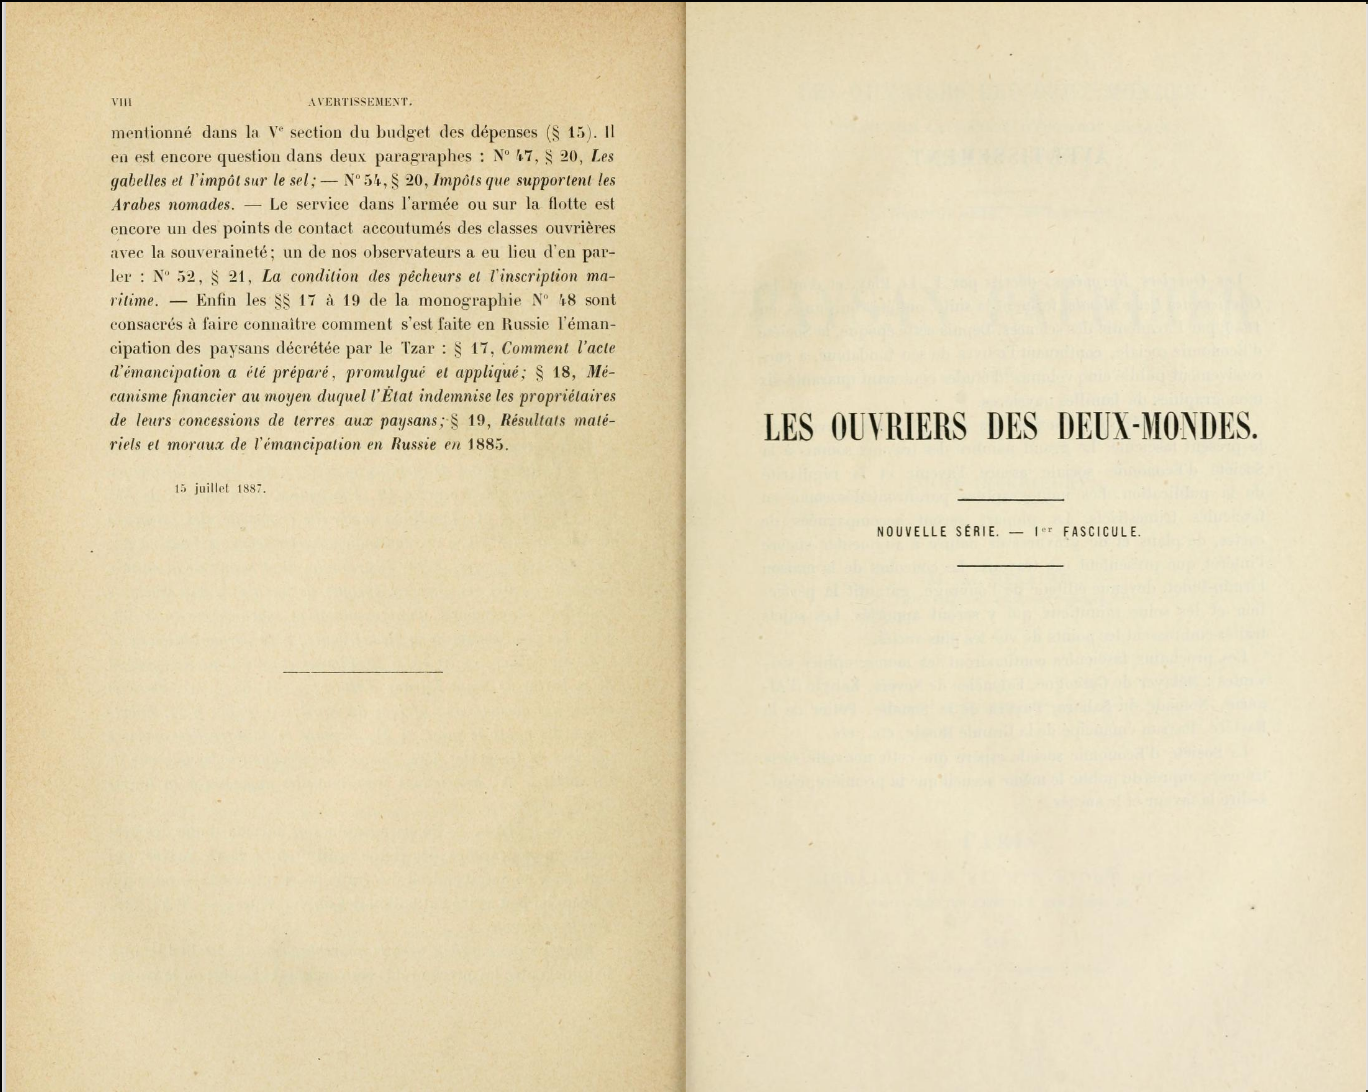
\includegraphics[width=1\linewidth]{img/odm47_ia_1.png}
     \caption{}
     \label{odm47ia1}
    \end{subfigure}
    \hspace{5pt}
    \begin{subfigure}[t]{0.4\textwidth}
     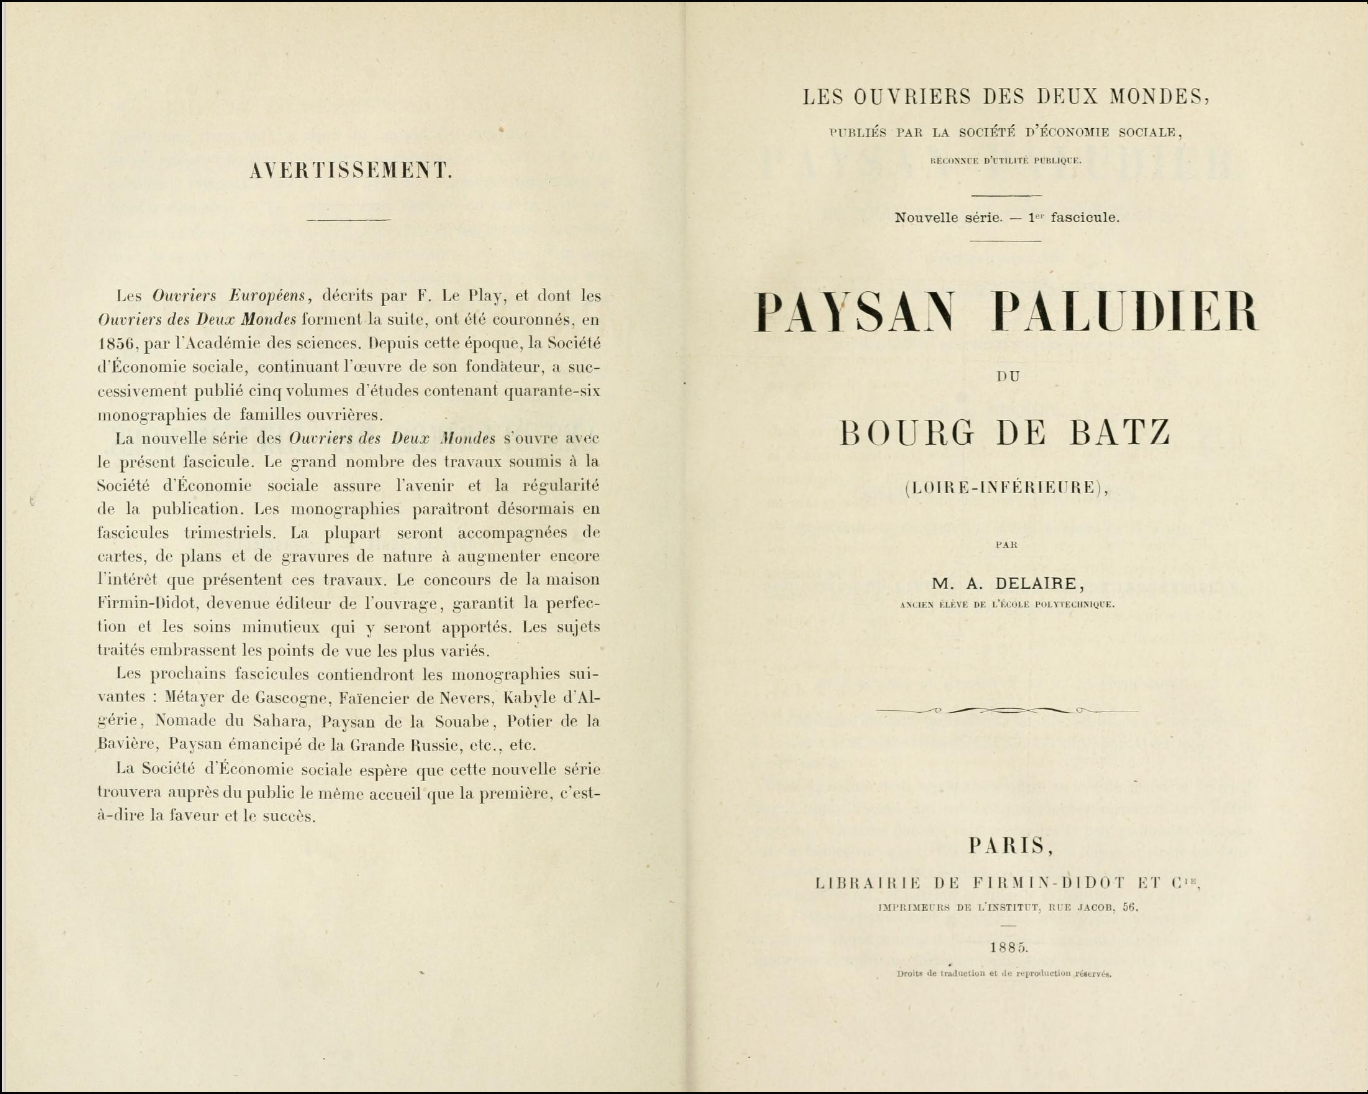
\includegraphics[width=1\linewidth]{img/odm47_ia_2.png}
     \caption{}
     \label{odm47ia2}
    \end{subfigure}
    \hspace{5pt}
    
    
    
    \begin{subfigure}[t]{0.4\textwidth}
     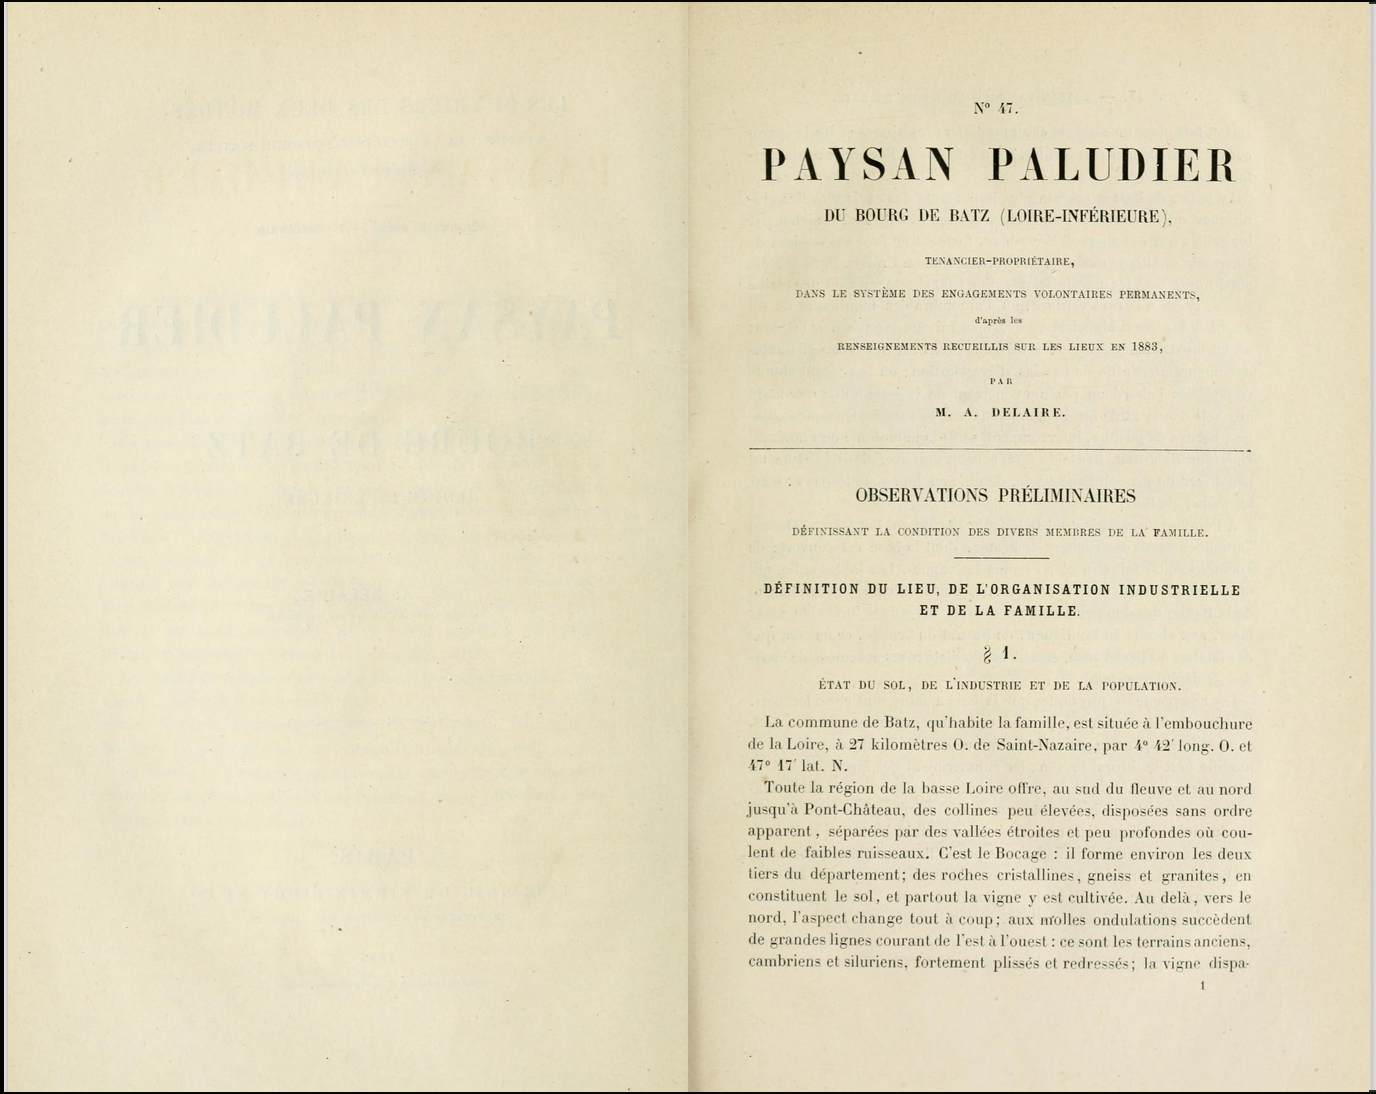
\includegraphics[width=1\linewidth]{img/odm47_ia_3.png}
     \caption{}
     \label{odm47ia3}
    \end{subfigure}
    \hspace{5pt}
    \begin{subfigure}[t]{0.4\textwidth}
     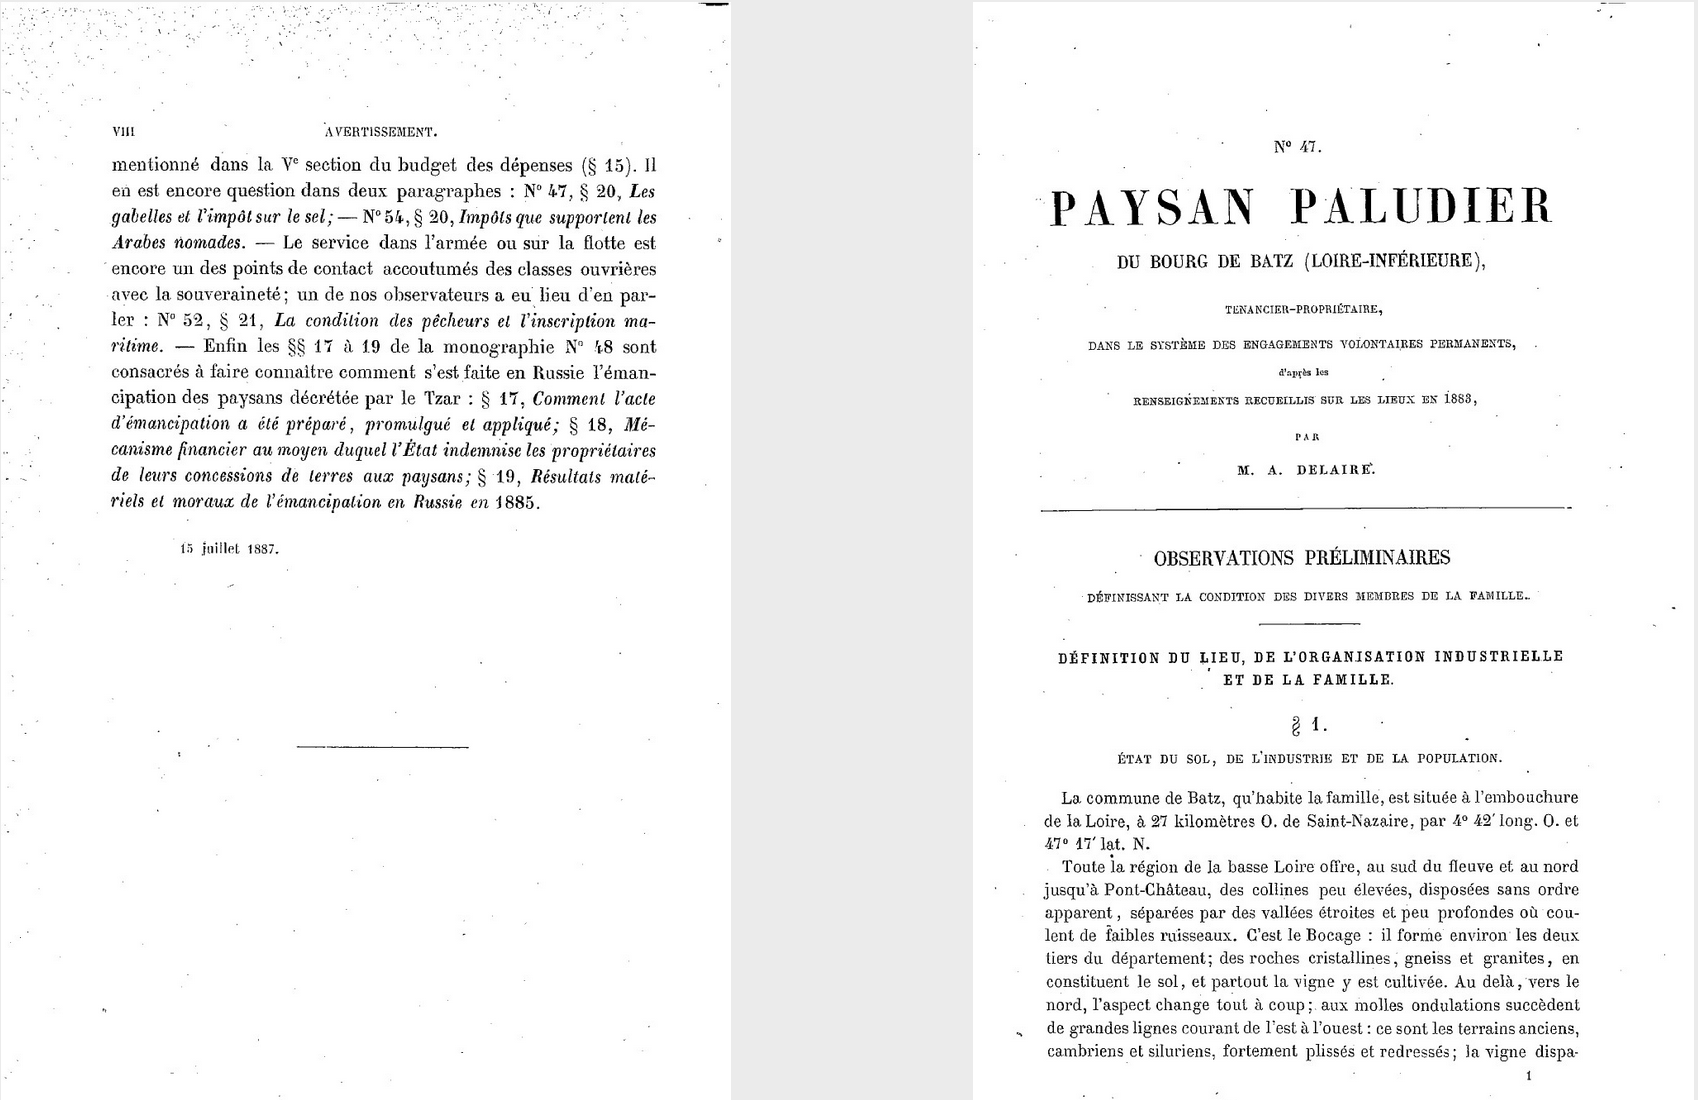
\includegraphics[width=1\linewidth]{img/odm47_bnf_1.png}
     \caption{}
     \label{odm47bnf}
    \end{subfigure}
    \caption[Comparaison des exemplaires de Toronto et de Paris]{Comparaison des exemplaires de Toronto et de Paris. (a)~Toronto. Fin de l'\textit{Avertissement} général du volume et début du fascicule. (b)~Toronto. \textit{Avertissement} du fascicule et page de titre de la monographie. (c)~Toronto. Début de la monographie. (d)~Paris. Fin de l'\textit{Avertissement} général du volume et début de la monographie.}
    \label{odm47}
\end{figure}

Deux versions de ce même volume sont à notre disposition. L'une résulte de la numérisation de l'exemplaire déposé à la Bibliothèque nationale de France à Paris et conservé par le département Philosophie, histoire, sciences de l'homme\footnote{Consultable sur \textit{Gallica} : \url{https://gallica.bnf.fr/ark:/12148/bpt6k54465138} (consulté le \today).}, la seconde se trouve à l'Université de Toronto et a été numérisée par \ia\footnote{Consultable à cette adresse : \url{https://archive.org/details/s2lesouvriersdes01sociuoft} (consulté le \today).}.

Des différences de composition existent et concernent notamment l'emplacement des page liminaires des fascicules. Ainsi, dans l'exemplaire de Toronto (\fig{} \ref{odm47ia1}, \ref{odm47ia2}, \ref{odm47ia3}), les premières pages ont été laissées à leur emplacement : la première porte au recto le titre des \odm{} et au verso l'\textit{Avertissement} que nous avons cité, la seconde est la page de titre du fascicule avec un verso vierge. Dans l'exemplaire de la Bibliothèque nationale, la première page de la monographie \no{}47 suit la fin de l'\textit{Avertissement} général du volume : deux feuillets sont donc manquant. Ils ont été éliminés lors du processus de reliure. Les mêmes manques s'observent dans les volumes qui suivent ; on peut cependant observer que les pages propres aux fascicules ont été placées en fin de volume, après la table des matières. Il n'y a donc pas eu d'élimination systématique.

Un autre élément symptomatique de ces différences de composition se remarque dans le corpus de Toronto. La monographie \no{}56 est la première du deuxième volume de la deuxième série\footcite{mono056a}, or elle se trouve également à la fin du volume précédent. La table des matières de ce dernier n'y fait pourtant pas référence. Ce doublon trouve sans doute son origine dans l'existence d'un fascicule surnuméraire que le relieur a choisi de conserver, quitte à l'implanter au mauvais endroit.

Ces exemples illustrent le fait que laisser aux acheteurs le soin de relier les fascicules pour composer le volume final revient à éloigner ce dernier de l'\oe{}uvre originelle, chaque nouvelle opération de reliure donnant naissance à un nouveau document. Les relieurs ont en effet pu choisir de conserver ou de ne pas conserver les pages propres aux fascicules, à l'instar des feuillets de l'exemplaire de Toronto. Il n'existe donc pas un modèle ayant autorité dans la composition des \odm{} --- en dépit du fait que les volumes de la Bibliothèque nationale de France, issus du dépôt légal, ont dû être versés par l'éditeur, \cad{} la Société internationale des études pratiques d'économie sociale.

Pour le projet \timeus{}, cela signifie que le corpus retenu pour le traitement informatisé et la publication finale ne peut être qu'une version de l'\oe{}uvre que représente les \odm.

\section{La structure logique des monographies}

Un élément remarquable traverse la centaine de monographies des \odm{} : une même structure logique que les éditeurs ont tenté de maintenir tout au long de la publication.

Cette structure est l'incarnation de la méthodologie leplaysienne des monographies de familles. Le terme \textit{monographie}, \og emprunté à l'histoire naturelle et à la médecine \fg{}, qualifie au \textsc{xix}\ieme ~siècle une \og étude scientifique, minutieuse et détaillée, portant sur un objet ou un phénomène circonscrit \fg{}\footnote{\cite[p. 12]{savoye2}.}. La démarche monographique cherche à embrasser à travers l'observation directe des phénomènes inatteignables pour la démarche statistique, à laquelle elle s'oppose\footnote{Voir en particulier la charge de F. Le Play contre les statisticiens dans son introduction aux \textit{Ouvriers européens} de 1855 : \og La méthode des statisticiens n'est pas l'observation directe des faits ; c'est la compilation et l'interprétation plus ou moins plausible de faits recueillis à des points de vue fort différents, étrangers pour la plupart à l'intérêt scientifique. Malgré leur généralité apparente et leur séduisante régularité, les statistiques ont médiocrement contribué au progrès de la science sociale \fg{} : \cite[p.~11]{oe1855}.}.

Avant les \odm, Frédéric Le Play s'attelle aux \textit{Ouvriers européens}, recueil paru en 1855 et réédité de 1877 à 1879. Cette série contient trente-six (1\iere{}~éd.) puis cinquante-sept (2\ieme{}~éd.) monographies issues d'enquêtes menées entre 1833 et 1853\footnote{Inventaire complet dans \cite[p. 106-112]{lorry}.}. Les \odm{} se présentent comme une suite élargie à des espaces extra-européens de ce premier mouvement, dont ils reprennent la démarche, la structure et auquel ils font régulièrement référence par un système de renvoi. La structure logique des \odm{}, dont le premier volume est publié en 1855, est donc déjà présente dans \textit{Les Ouvriers européens}.

Elle procède d'une méthode d'observation sur laquelle Le Play revient en 1862, au moment de la parution du quatrième volume des \odm{}. Le titre de cette méthodologie précise néanmoins qu'elle a déjà fait ses preuves pour les \textit{Ouvriers européens} : \textit{Instruction sur la méthode d'observation dite des monographies de familles, propre à l'ouvrage intitulé} Les ouvriers européens\footcite{instruction62}.

L'\textit{Instruction} est divisée en quatre parties suivies d'une cinquième faisant office de conclusion. Dans la première, Le Play circonscrit son champ d'observation à la famille ouvrière\footcite[I., \og Remarques préliminaires sur l'étude des faits sociaux et sur la méthode des monographies de familles \fg{}, p. 15-16]{instruction62}, érigée en \og clef de compréhension des organisations sociales \fg{}\footcite[p. 15]{savoye2}. La phase d'observation est ensuite divisée en étapes \footcite[II., \og Règles à suivre pour procéder à l'observation des faits sociaux \fg{}, p. 17-19]{instruction62}, savoir l'observation des faits, l'interrogatoire de l'ouvrier et celui des personnes tiers\footcite[p. 16]{savoye2}.

La troisième partie est celle où Le Play expose la structure logique qu'il utilise à partir de 1855 et que ses \og continuateurs \fg{}\footnote{Nous désignons par ce terme le groupe d'individus qui a participé à l'entreprise des \odm{} après la mort de Le Play, sans entrer dans les débats sur l'existence ou non d'une \og école leplaysienne \fg{}. De fait, un schisme a lieu à la fin des années 1880 : \cite{savoyecontinuateurs}.} reprennent jusqu'en 1930. Elle est construite en miroir aux différentes phases de l'observation sur le terrain : à l'observation des faits répond la section des\textit{ Observations préliminaires}, à l'interrogatoire de l'ouvrier celle des \textit{Budgets} et aux contacts avec les tiers celle des \textit{Notes}\footcite[III., \og Précis des faits à observer --- Établissement des budgets \fg{}, p. 20-31]{instruction62}.

Le miroir est cependant légèrement déformant, afin de satisfaire au \og hiatus \fg{} propre à la démarche leplaysienne, qui différencie les \og faits observés \fg{} des \og faits décrits \fg\footcite[p. 87]{baciocchi2}. L'observation est en effet \og contrainte par l'évidence des choses \fg{} là où la description, \og parce qu'elle suppose de désigner précisément ce qu'on évoque, repose sur un calibrage sémantique \fg{}\footcite[p. 87-88]{baciocchi2}. Les monographies se trouvent du côté de la description des faits, leur structure logique n'est donc pas qu'un simple plan de rédaction, elle procède d'une démarche intellectuelle réglée par Le Play qui doit être appliquée pour garantir la validité de la démonstration.

Cette structure (\ann{} \ref{structure}) possède trois niveaux de titre : les parties~(A, B, C), les sections~(I, II, etc.) et les paragraphes~(§1, §2, etc.). La partie~C (\textit{Notes}) n'a pas recours au deuxième niveau et ne contient que des paragraphes.

\begin{figure}[ht]
    \centering
    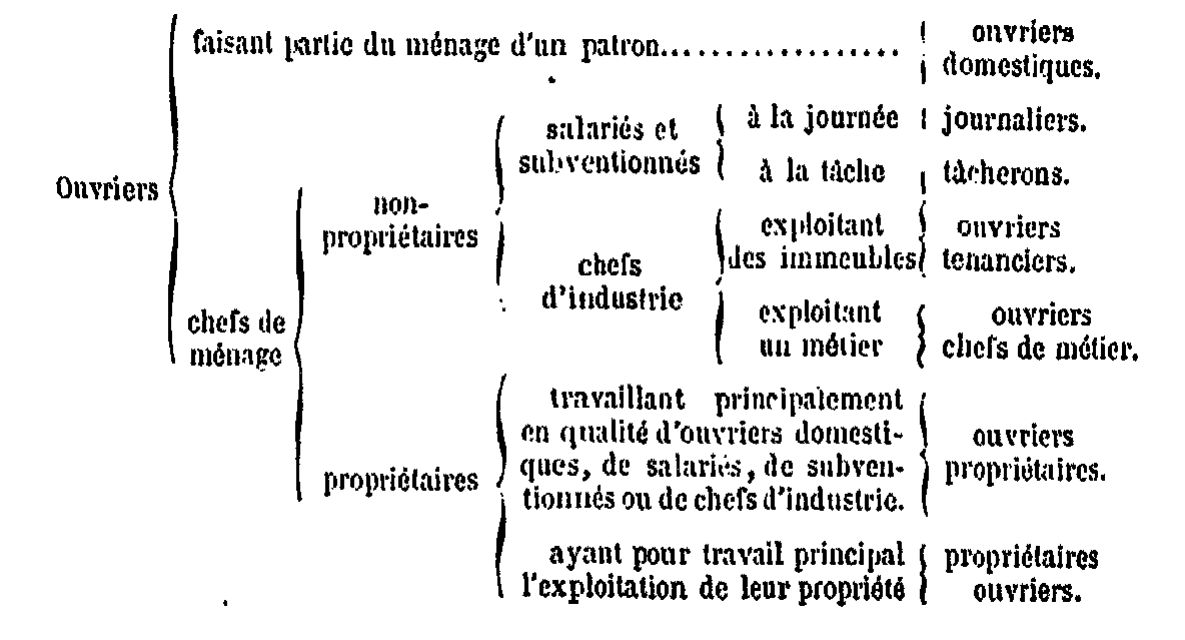
\includegraphics{img/tabl_titres.jpg}
    \caption[Tableau des sept situations principales que les ouvriers peuvent occuper successivement]{\og Tableau des sept situations principales que les ouvriers peuvent occuper successivement dans les quatre systèmes sociaux pour s'élever des rangs inférieurs de la hiérarchie industrielle à la condition de propriétaires ou de chefs d'industrie. \fg{}, permettant de construire le titre d'une monographie de famille (capture d'écran de \textit{Gallica}).}
    \label{tabletitre}
\end{figure}

La première partie~(A) est la page de titre. Le titre de la monographie est présenté comme le \og résumé \fg{} de celle-ci, et doit pour cela contenir quatre éléments imprescriptibles : \og 1° la profession de l'ouvrier, 2° la population dont il fait partie, 3° la nature des engagements qu'il contracte pour se procurer des moyens de travail, 4° la situation qu'il occupe dans l'organisation sociale caractérisée par cet engagement \fg{}\footcite[p. 20]{instruction62}. Ainsi, en dépit du fait que Le Play ne considère pas explicitement la page de titre comme une composante de sa structure, l'importance qu'il donne au titre en lui-même a conduit le projet \timeus{} à l'interpréter comme telle. Un tableau pour construire ce titre est d'ailleurs mis à la disposition des monographes (\fig{} \ref{tabletitre}\footcite[p. 21 .]{instruction62}).

\section[Continuité et discontinuité]{Continuité et discontinuité dans la structure logique}

En dépit de son aspect monolithique, la structure logique des monographies de familles subit plusieurs ajustements au cours de la publication. Certains, uniquement de circonstance, sont des évènements mineurs, là où d'autres sont des changements significatifs adoptés pour la suite de la publication.

La monographie \no{}85 représente ainsi un tournant dans la numérotation des titres de paragraphe, sans pour autant changer leurs libellés (\ann{} \ref{structure}). En effet, la numérotation cardinale est étendue au dernier paragraphe des budgets (\textit{Comptes annexés aux budgets}) et remplace la numérotation alphabétique utilisée auparavant dans la partie \textit{Notes}.

Pourquoi cette uniformisation intervient-elle à partir de cette monographie, en plein milieu du cinquième volume ? Nous avons vu plus haut qu'il représentait un tournant dans la publication des \odm, notamment en raison de la mort de Frédéric Le Play qui intervient avant qu'il ne soit achevé. Il est possible que le départ du fondateur de la série ait permis d'opérer des changements dans la structure qu'il avait créée, ou bien que ce soit Le Play lui-même qui ait souhaité ces changements. Quoi qu'il en soit, il y a une volonté claire de renforcer la solidité de la démonstration en rassemblant ces différents paragraphes en un seul bloc par le biais d'une numérotation cardinale continue. Le nombre moyen de paragraphes est de vingt-et-un ; la monographie la plus longue, composée de trente-cinq paragraphes, étant la \no{}64, intitulée \textit{Paysans corses en communauté, porchers-bergers des montagnes de Bastelica}\footcite{mono064a}.

Ce même volume est l'occasion pour la \sess{} d'agréger aux \odm{} un type de monographie déjà introduite dans la ré-édition des \textit{Ouvriers européens} (1877-1879), le précis\footcite[p. 102]{lorry}. Elle le définit comme un document qui, \og n'ayant pas la forme complète des travaux auxquels ce recueil est destiné [les monographies de familles], offre néanmoins assez d'intérêt pour avoir été annexé à la description d'une famille de même nationalité \fg{}\footcite[p. II]{averts2t1}. Il s'agit d'un texte court, d'une quinzaine de pages environ, qui, tout en ayant le même propos qu'une monographie, est fortement \og allégé \fg{}\footcite[p. 7]{chenu}.

Cet allègement se remarque à travers deux traits caractéristiques. Le premier est la suppression du paragraphe 16 et la réduction des paragraphes 14 et 15 consacrés aux budgets. Ils sont en effet réduits à quelques lignes, là où il s'agit de tableaux de plusieurs pages dans les  monographies de familles. Le précis \no{}92 \textit{bis} est le seul à posséder un paragraphe 16, mais les 14 et 15 sont rassemblés en une seule section\footcite[p. 78-81]{mono092b}. Le second trait caractéristique consiste en des notes extrêmement courtes (un à trois paragraphes, à l'exception du précis \no{}66 \textit{ter} qui en compte six\footcite[p. 158-172]{mono066c}).

Les libellés des titres peuvent également être modifiés. Celui de la deuxième partie (\textit{Observations préliminaires}) est absent des précis \no{}~58 \textit{bis}\footcite[p. 153]{mono058b} et 66~\textit{bis}\footcite[p. 125]{mono066b}. Ceux des paragraphes sont également placés en italique au début du texte dans quatre précis (\no{} 58~\textit{bis}, 66~\textit{bis}, 85~\textit{bis}\footcite{mono085b}, 90~\textit{bis}\footcite{mono090b}).

Les trois premiers précis sont des cas particuliers, puisqu'à l'inverse des suivants ils ne sont pas formellement détachés de la monographie dont ils découlent (\no{}~41\footcite[p. 188-196]{mono041a}, 42\footcite[246-258]{mono042a} et 43\footcite[p. 300-305]{mono043a}) mais sont traités comme une section de la partie \textit{Notes}. Il n'y a ni grandes parties ni titres de paragraphe, seul le niveau intermédiaire ayant été retenu : les sections I à IV dans les trois, et un court budget dans les deux derniers.

Un dernier facteur de discontinuité au sein des \odm{} et de sa structure logique doit être signalé : il s'agit des deux monographies d'ateliers que l'on trouve dans la troisième série. La première s'intéresse à la société générale des papeteries du Limousin (1904\footcite{mono472a}) et la seconde à  une usine hydraulique d’éclairage et de transport de force sur la Loire (1908\footcite{mono473a}). La monographie d'atelier est théorisée par Émile Cheysson, une des grandes figures de la \sess après la mort de Le Play\footcite[p. 336-337]{savoyecontinuateurs}, pour qui le \og foyer cesse d'être le centre unique de notre activité et cède à l'atelier une partie de ses attributions primitives \fg{}\footnote{Émile Cheysson, \og La monographie d'atelier et les Sociétés d'économie sociale \fg{}, \textit{La Réforme sociale}, 15 mai 1887, p. 545 --- cité dans \cite[p. 23]{savoye2}.}.

Il s'agit d'une rupture importante avec l'objectif initial des \odm, mais également d'un signe de la volonté de la collection de s'adapter à son temps. Ces deux textes ne peuvent néanmoins pas reprendre la structure logique initiale, uniquement applicable aux familles. Néanmoins, on trouve dans leur organisation des traits similaires : trois parties (\textit{Organisation commerciale de l'atelier}, \textit{Organisation du travail} et des \textit{Appendices} faisant fonction de notes), un second niveau signalé par une numérotation en romain et des paragraphes qui peuvent être titrés ou non\footcite[p. 337]{savoyecontinuateurs}.

Ces modulations dans l'application de la structure définie par Frédéric Le Play sont importantes pour le projet \timeus. Son but étant de mettre à la disposition de la communauté scientifique les monographies des \odm{} sous la forme de fichiers XML-TEI, il est nécessaire qu'il étudie cette structure et qu'il fasse la part entre ses moments de continuité et de rupture. Ceux-ci doivent en effet être pris en compte dans l'établissement du schéma d'encodage.

\newpage
\thispagestyle{empty}
\mbox{}
\newpage

\chapter{Des numérisations multiples}

Avant d'établir le schéma d'encodage des \odm, il est nécessaire de disposer d'une version digitale du corpus \og papier \fg{} pour réaliser une opération de transcription automatique. Or, comme nous l'avons déjà signalé, les \odm{} ont bénéficié des programmes de numérisation des ressources des bibliothèques.

Un corpus se trouve notamment sur le site \gb, mais il n'est important que d'un \pov{} quantitatif et non pas qualitatif. En effet, les treize volumes ne sont pas accessibles dans leur intégralité. Cet accès restreint est regrettable, dans la mesure où \gb{} n'a pas numérisé un seul corpus, mais plusieurs issus de bibliothèques italiennes, françaises et américaines (\ann{} \ref{numgb}). Disposer de tous ces exemplaires aurait permis un relevé plus fin des différences de composition. Notons que par l'intermédiaire de la \textit{HathiTrust Digital Library }, une bibliothèque numérique lancée en 2008 et agrégeant les livres numérisés par \gb, \ia{} et certaines bibliothèques universitaires, il est possible de consulter à des numérisations pour lesquelles l'accès est restreint par Google.

Le projet \timeus{} s'est donc orienté vers les deux seuls corpus complets, hébergés par la Bibliothèque nationale de France et le site \ia.

\section{Les volumes de la Bibliothèque nationale de France}

Les trois séries des \odm{} ont été mises en ligne sur le site \textit{Gallica} de la Bibliothèque nationale de France le 15 octobre 2007\footnote{Notice de la numérisation : \url{https://gallica.bnf.fr/ark:/12148/cb32830863r/} (consulté le \today).}.

Les volumes sont téléchargeables en trois formats :

\begin{itemize}
    \item PDF (\textit{Portable Document Format}), qui préserve la mise en page du document telle qu'elle a été définie par son auteur ;
    \item TXT, qui contient uniquement du texte brut, \cad{} des chaînes de caractères (ce qui n'intéresse pas le programme \timeus, qui souhaite obtenir les images des pages de chaque volume) ;
    \item JPEG (\textit{Joint Photographic Experts Group}), qui permet de compresser les images avant de les enregistrer.
\end{itemize}

Le téléchargement au format JPEG n'est possible que pour la page en cours de visualisation par l'utilisateur. Seul le téléchargement au format PDF permet d'obtenir l'ensemble des images, avec l'inconvénient qu'elles sont toutes rassemblées en un seul fichier, ce qui complique le traitement à la chaîne.

Le corpus numérisé sur \textit{Gallica} n'est ainsi pas exploitable par le programme \timeus. Cela est regrettable dans la mesure où, comme nous l'avions signalé plus haut, il s'agit des exemplaires issus du dépôt légal et donc déposés par l'éditeur des \odm. Il s'agissait de l'unique occasion d'avoir avec certitude la vision que Frédéric Le Play et la \sess{} avaient de leur travail.

\section{Les volumes d'\ia}

\ia{} est un organisme privé à but non lucratif fondé en 1996 par Brewster Kahle. Son objectif premier, tel qu'annoncé dans son \textit{manifeste}, est de \og collecter les données publiques sur Internet pour bâtir une bibliothèque digitale \fg{}\footnote{\og \textit{The Internet Archive is such a new organization that is collecting the public materials on the Internet to construct a digital library} \fg{} : \cite{Brewster1} (cité dans \cite{Brewster2}).}. Cet archivage du web est accessible grâce à l'outil \textit{Wayback Machine}, lancé en octobre 2001\footcite[p.344]{panos} mais prévu dès le lancement d'\ia\footnote{\textit{We possess the capability of supplying documents that are no longer available from the origi- nal publisher, an important function if the Web’s hypertext system is to become a medium for scholarly publishing. Such a service could also prove worthwhile for business research.} : \cite[p.83]{iamanifest}.}. À partir de 2000, l'organisation commence à archiver les programmes de télévision, les musiques et les films numériques~; en 2001, c'est au tour des livres de faire leur entrée sur ses serveurs\footcite[p. 3-4]{Brewster2}.

\ia{} commence ses digitalisations en tant que participant au projet \textit{Million Book} de l'Université Carnegie-Mellon de Pittsburgh, et se met à digitaliser par lui-même en se rendant dans les bibliothèques universitaires à partir de 2005\footcite[p. 4]{Brewster2}. La digitilasation est faite page par page au moyen de scanners\footcite[p. 4]{Brewster2}. Les livres ainsi numérisés sont accessibles  et téléchargeables librement, sans aucune restriction, ce qui constitue le principal avantage du site, à l'image de \textit{Gallica} et à l'inverse d'autres plates-formes comme \gb\footcite[p. 1]{Brewster2}. Par rapport à \textit{Gallica}, \ia{} offre beaucoup plus de formats pour le téléchargement de ses fichiers\footnote{Liste complète : \cite[p. 33]{chague}.}.

Les exemplaires des \odm{} numérisés sur \ia{} sont conservés à la \textit{John P. Robarts Research Library} de l'Université de Toronto. Leurs mises en ligne ont été réalisées en novembre 2008, mise à part le fascicule 17 \textit{bis} de la série 3, ajouté en mars 2010.

\section{Choix du corpus à numériser}

\begin{figure}[ht]
    \centering
    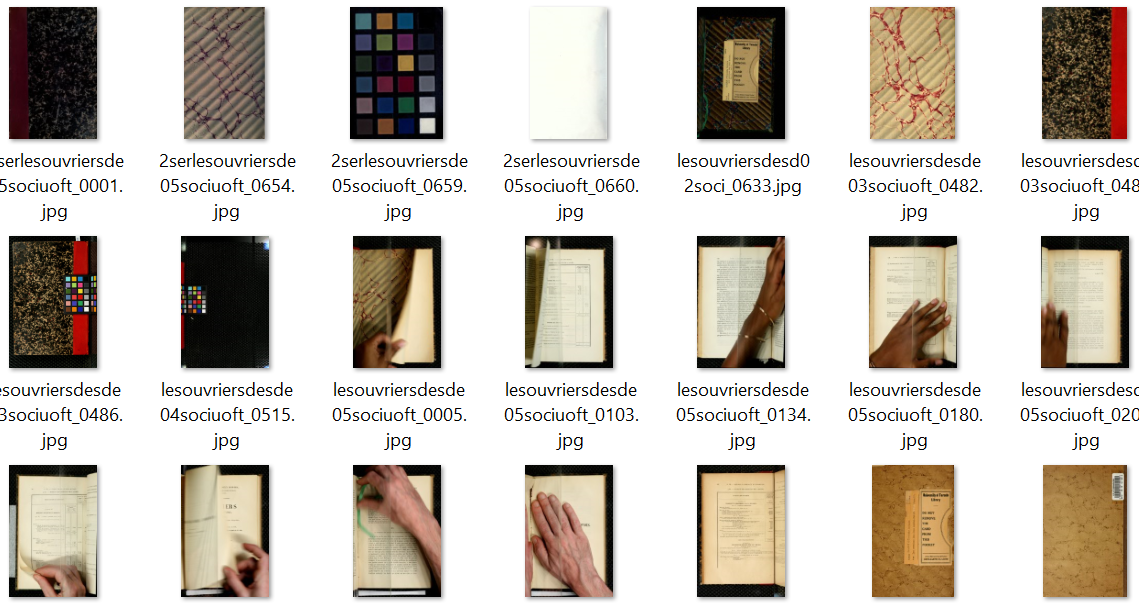
\includegraphics[width=15cm]{img/ex_tri.png}
    \caption[Images exclues du lot à transcrire]{Exemples d'images exclues du lot à transcrire (source : Alix Chagué, \url{https://timeus.hypotheses.org/626}).}
    \label{fig:ex_tri}
\end{figure}

Le téléchargement depuis \ia{} permet d'obtenir un dossier contenant le fichier image de chaque page au format JPEG (en l'occurrence JPEG 2000, abrégé en JP2) avec une qualité maximale\footcite{chague2}. C'est donc pour ce corpus et ce format qu'a opté le programme \timeus. Cela représente 7 190 fichiers images, pour un poids de 3,3 Go\footcite{chague2}.

L'ensemble a été versé sur un espace de stockage créé grâce au service \sharedocs{} de la TGIR Huma-Num. Adopté en mai 2018 à l'initiative de l'équipe ALMAnaCH, ce service est gratuit, français et sur-mesure (l'espace de stockage est alloué à la demande)\footcite[p. 33-34]{chague2}. Le \sharedocs{} permet également de centraliser l'ensemble des fichiers image du programme \timeus.

Choisir le corpus d'\ia{} n'est pas sans conséquence, notamment en raison du caractère incomplet du corpus. Les fascicules contenant les six dernières monographies (\nos{}~109 à 114) et les précis qui les accompagnent (\nos{}~109~\textit{bis} à 111~\textit{bis}) n'ont en effet pas été numérisés. De fait, nous ne les avons trouvés qu'à une seule adresse sur Internet : il s'agit de l'exemplaire de l'Université de Princeton numérisé par \gb{} et accessible par le truchement de la \textit{HathiTrust Digital Library} (\ann{} \ref{numgb}). Il contient les monographies \nos{}~108 à 112 et constitue donc le troisième volume de la troisième série. Nous n'avons pas trouvé d'exemplaires numérisés des deux dernières monographies, publiées à la fin des années 20 du \textsc{xx}\ieme~siècle. \textit{[Erratum, novembre 2020 : l'avant dernière monographie, datée de 1928, est numérisée sur Gallica.]}

Ce corpus comporte également divers biais liés à l'impression, dont des titres appartenant à la structure logique qui n'ont pas été imprimés (\ann{} \ref{ann:deficit-transcr}), sans que l'on puisse déterminer s'il s'agit d'une erreur de composition ou d'une suppression volontaire par les éditeurs. 

Notons qu'en dépit de ces écueils, toutes les monographies relatives au textile et qui intéressent directement le programme \timeus{} sont présentes dans le corpus d'\ia.

À l'issue du téléchargement, il a fallu procéder à un contrôle de la qualité des fichiers, afin de détecter et de retirer les images présentant des imperfections\footcite{chague2}. Ces dernières étaient principalement dues à des erreurs de cadrage ou à des vues prises alors que la main de l'opérateur ou de l'opératrice était toujours présente dans le champ de l'image (\fig{} \ref{fig:ex_tri}).

\begin{figure}[ht]
    \centering
    \begin{subfigure}[t]{0.4\textwidth}
     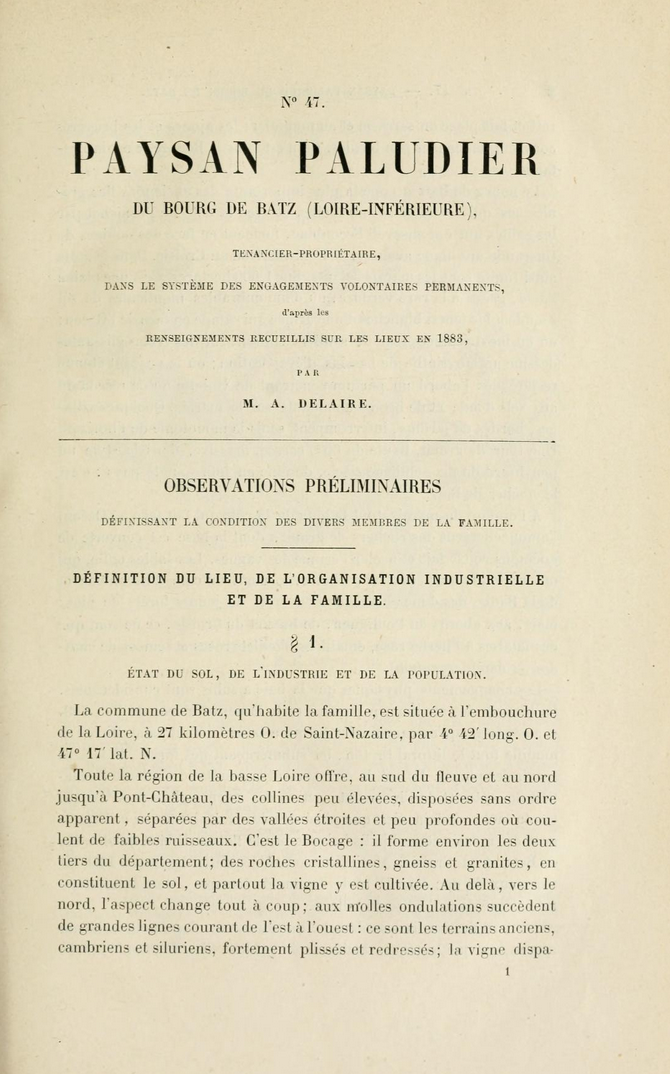
\includegraphics[width=0.7\linewidth]{img/title_s2t1_m47_p1.png}
    \end{subfigure}
    \hspace{5pt}
    \begin{subfigure}[t]{0.4\textwidth}
     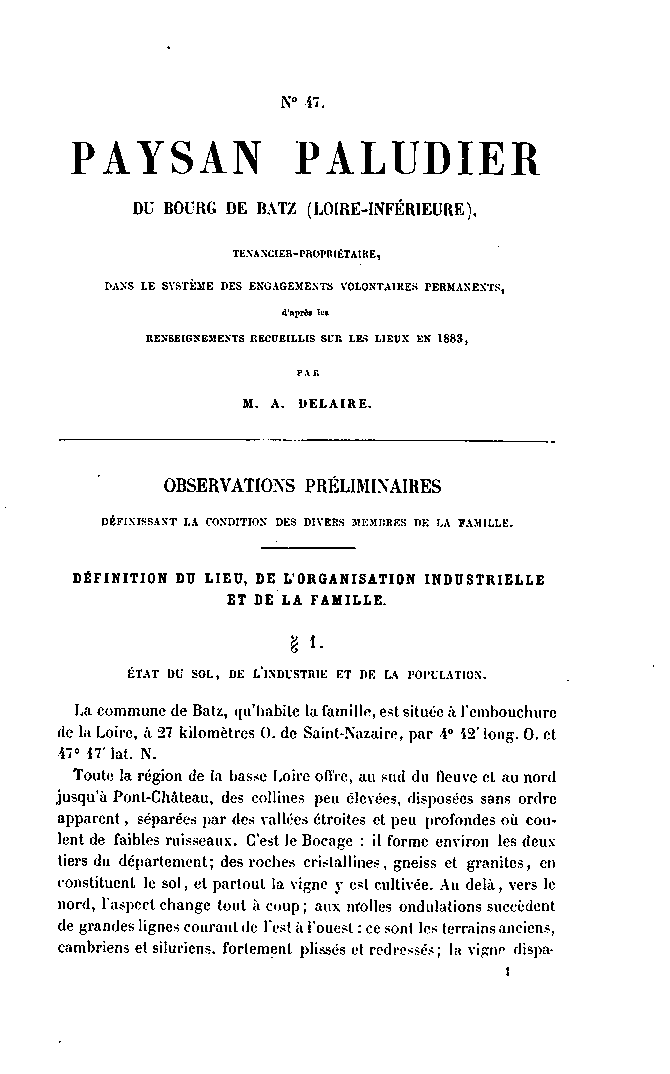
\includegraphics[width=0.7\linewidth]{img/title_binarize.png}
    \end{subfigure}
    \caption[Exemple d'une binarisation]{Exemple d'une binarisation : s. 2 vol. 1, \no{} 47, p. 1.}
    \label{fig:binarisation}
\end{figure}

Enfin, les images retenues ont été binarisées, \cad{} passées en valeur de noir ou blanc (\fig{} \ref{fig:binarisation}). Cette opération permet d'augmenter la qualité des textes et donc leur détection par les programmes de transcription automatique. Un autre avantage est qu'elle supprime les annotations manuscrites, par exemple celles ajoutées par les agents des bibliothèques et relatives au classement du volume.

Dès lors que le corpus était nettoyé, les opérations de transcription et d'encodage pouvaient débuter.

\newpage
\thispagestyle{empty}
\mbox{}
\newpage

\chapter{Un encodage automatique}

\section{Choix de l'automatisation}
Le programme \timeus{} a choisi de procéder lui-même à la transcription des treize volumes des \odm{} et à l'encodage du texte brut ainsi obtenu. 

Cela n'était pas envisagé ainsi au départ, un budget ayant été prévu pour externaliser cette étape. Néanmoins, l'équipe ALMAnaCH d'Inria a fait valoir les risques inhérents à une telle opération, et notamment la difficulté à rédiger un cahier des charges suffisamment rigide pour pouvoir contrôler les différentes étapes de réalisation et les orientations scientifiques décidées lors de celles-ci.

Le choix s'est donc porté sur une réalisation en interne avec la possibilité de la conduire manuellement (un humain réalise les transcriptions avant de les encoder) ou automatiquement (un humain écrit un programme qui prend les images en entrée et fournit des fichiers XML en sortie)\footcite[p. 52]{chague}. La solution du travail manuel avait été envisagée dans un premier temps, notamment par le Centre Maurice-Halbwachs, grâce au recrutement d'un(e) ingénieur(e) d'études à temps plein pour six mois\footcite[p. 52]{chague}. 

ALMAnaCH a cependant proposé de prendre en charge l'écriture du programme permettant d'automatiser l'opération, en insistant sur les apports méthodologiques et scientifiques que cela représenteraient pour le programme\footcite[p. 52]{chague}. Le succès d'une telle opération lui permettrait en effet de développer ses compétences dans l'acquisition et l'encodage automatique de texte imprimé.

Ajoutons que cette proposition correspond à la dynamique interne dont nous avons constaté la prégnance sur les membres d'ALMAnaCH dès le début du stage. Une réflexion y est sy
stématiquement menée pour étudier l'opportunité d'automatiser les tâches répétitives dans un objectif évident de gain de temps, mais également de développement expérimental de nouvelles techniques de traitement des fichiers.

Pour mener à bien cette phase du programme, deux contrats d'ingénieur d'études de trois mois chacun (octobre à décembre 2018, février à mai 2019) ont été financés. La fiche de poste comptait sept missions\footnote{Informations transmises par Alix Chagué.} :

\begin{itemize}
    \item Réaliser un benchmark de toutes les solutions d'\ocr{} disponibles et adaptées pour le projet ;
    \item Établir une méthodologie de traitement des documents ;
    \item Télécharger les images, les contrôler et les pré-traiter ;
    \item Réaliser l'\ocr{} ;
    \item Analyser la structure logique des enquêtes pour identifier les indices textuels et typographiques permettant la structuration des transcriptions ;
    \item Établir un schéma TEI traduisant la structure logique ;
    \item Rédiger un programme cherchant ces indices et implémentant le schéma TEI.
\end{itemize}

\section{Le script \textsc{LSE-OD2M}}

La transcription automatique d'un document imprimé nécessite l'usage d'un logiciel d'\ocr{} (\textit{Optical Character Recognition}, en français \textit{reconnaissance optique de caractères}). Quatre étapes sont nécessaires afin d'obtenir un résultat satisfaisant : préparer les images en amont afin de faciliter la reconnaissance des caractères, segmenter l'image en zones d'information, extraire le texte et enfin contrôler et corriger le rendu\footcite[p. 1]{karpinski}.

Nous avons déjà évoqué la préparation des images dans le chapitre précédent, la correction correspondant quant à elle au travail produit pendant notre stage. Nous nous arrêterons donc sur les deuxième (segmentation) et troisième (transcription automatique) phases dans le propos qui suit, en y adjoignant la structuration du texte sous forme de fichiers XML-TEI.

Sur ces trois étapes, les deux dernières ont été entièrement prises en charge par un script Python dénommé \textit{Logical Structure Extraction from Les Ouvriers des Deux Mondes} (\lse), écrit par Alix Chagué de février à mai 2019.

\subsection{Segmentation}

Le but d'une segmentation est d'identifier dans l'image d'un texte des zones qui correspondent à des sous-ensembles logiques de ce texte. Il peut s'agir de paragraphes, de lignes ou de mots, la granularité pouvant être poussée jusqu'aux caractères\footcite[p. 3]{karpinski}. Ce moment est crucial pour l'\ocr, puisque la reconnaissance des caractères s'effectuera sur les zones ainsi segmentées\footcite[p. 3]{casey}. Il est identifié depuis de nombreuses années\footcite[p. 4]{casey} comme une source majeure des erreurs présentes dans le résultat final\footcite[p. 120]{elagouni}.

Plusieurs caractéristiques des \odm{} facilitent leur transcription. D'une part, il s'agit d'un imprimé du \textsc{xix}\ieme ~siècle, ce qui garantit un texte relativement régulier dont l'alphabet correspond au nôtre (les \textit{s} sont ronds et non longs). D'autre part, les pages sont organisées en une seule colonne. Les erreurs \og de fusion \fg{}, par exemple un texte dont les deux colonnes seraient identifiées comme un seul bloc, ne peuvent pas survenir\footcite[p. 5]{karpinski}.

\begin{figure}
    \centering
    \begin{subfigure}[t]{0.4\textwidth}
     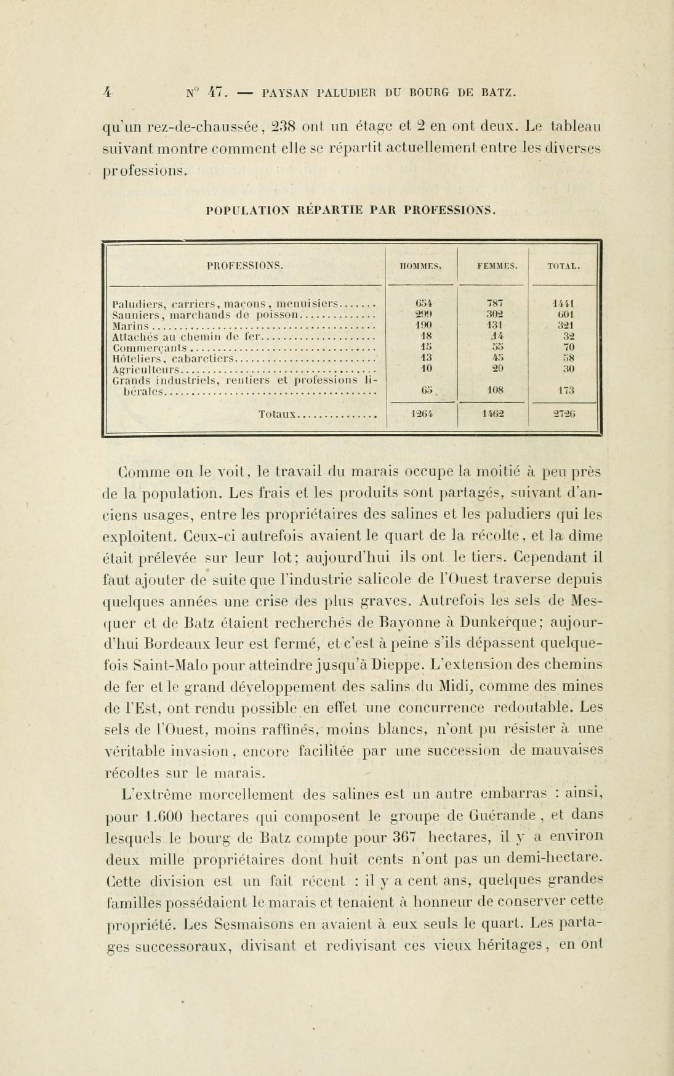
\includegraphics[width=0.8\linewidth]{img/tabl_s2t1_m47_p4.png}
     \caption{s. 2 vol. 1, \no{} 47, p. 4.}
    \end{subfigure}
    \hspace{5pt}
    \begin{subfigure}[t]{0.4\textwidth}
     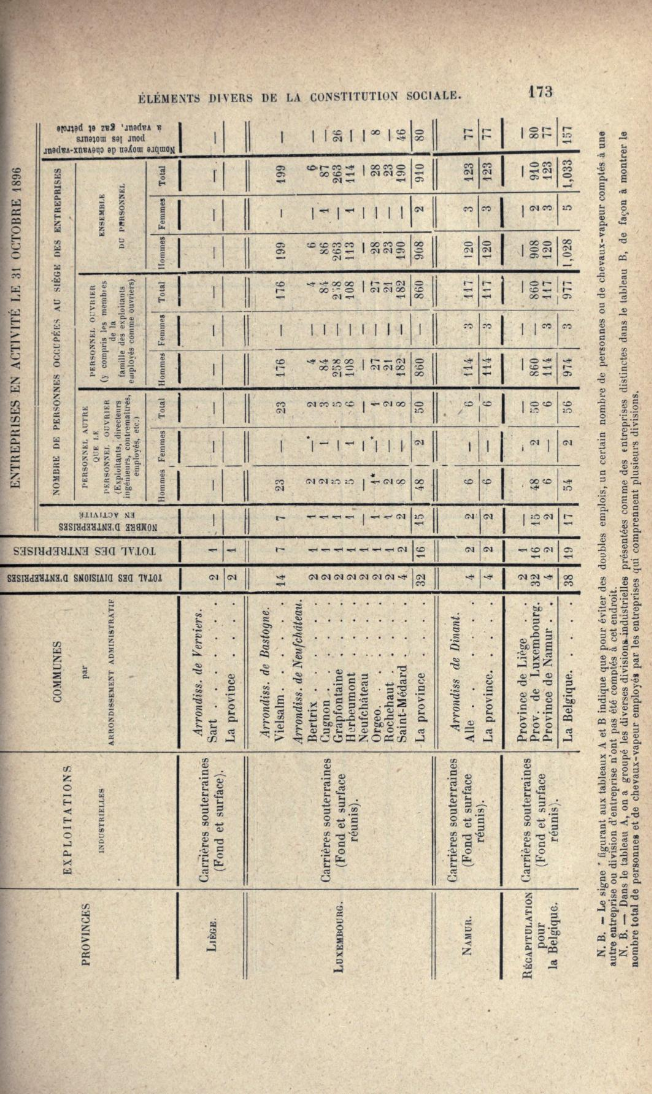
\includegraphics[width=0.8\linewidth]{img/tabl_s3t1_m102_p173.png}
     \caption{s. 3 vol. 1, \no{} 102, p. 173.}
     \label{fig:ex_figures:table}
    \end{subfigure}
    \hspace{5pt}
    
    
    
    \begin{subfigure}[t]{0.4\textwidth}
     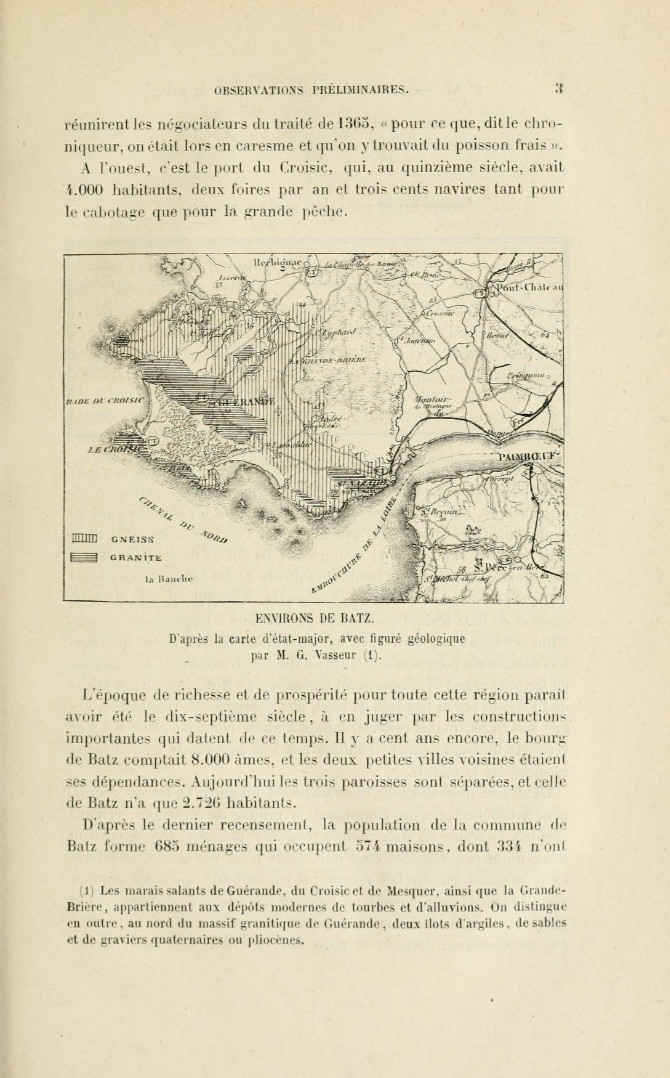
\includegraphics[width=0.8\linewidth]{img/map_s2t1_m47_p3.png}
     \caption{s. 2 vol. 1, \no{} 47, p. 3.}
    \end{subfigure}
    \hspace{5pt}
    \begin{subfigure}[t]{0.4\textwidth}
     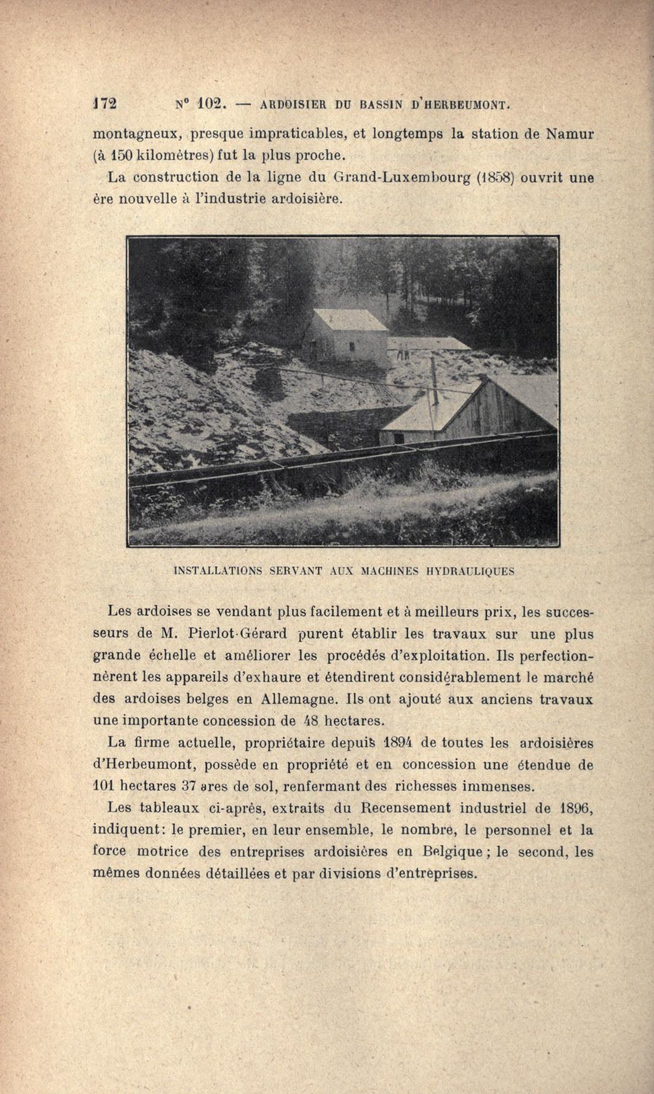
\includegraphics[width=0.8\linewidth]{img/img_s3t1_m102_p172.png}
     \caption{s. 3 vol. 1, \no{} 102, p. 172.}
    \end{subfigure}
    \hspace{5pt}
    \caption[Exemples d'objets graphiques]{Exemples d'objets graphiques dans les pages des \odm{}.}
    \label{fig:ex_figures}
\end{figure}

\lodm{} ne contiennent cependant pas que des chaînes de caractères organisées en lignes. On y trouve des \og objets \fg{} : outre des reproductions de photographies occupant tout ou partie de la page dans les monographies des deuxième et troisième séries, il s'agit principalement de tableaux (\fig{} \ref{fig:ex_figures}). Les paragraphes 14 à 16 consistent ainsi en des tableaux de budget qui s'étendent sur plusieurs pages. Ils suscitent un intérêt particulier pour le programme \timeus{}, dans la mesure où ces budgets permettent de reconstituer les différents postes de dépenses des familles --- et notamment le textile --- et les ressources qui leur sont allouées. Des tableaux peuvent également se trouver dans les autres sections, entre deux paragraphes.

La segmentation en elle-même a été réalisée à l'aide du logiciel \textit{\textsc{abbyy} FineReader}\footnote{\textit{FineReader} produit également une transcription, mais celle-ci est de trop mauvaise qualité pour pouvoir être exploitée}, en tant que service proposé par le logiciel \transkribus{}\footcite{chague2}. Ce dernier est une plate-forme de transcription et d’annotation développée par le programme européen \textsc{read} (\textit{Recognition and Enrichment of Archival Documents})\footnote{Présentation du logiciel : \url{https://readcoop.eu/transkribus/} (consulté le \today).}.

Un total de 6 668 images issues des \odm{} a été chargé dans \transkribus{}. \textit{FineReader} a ensuite analysé leur mise en page et fourni un résultat sous la forme d'un fichier XML ALTO\footcite{alto}. ALTO (\textit{Analyzed Layout and Text Object}) est un format maintenu par la Bibliothèque du Congrès qui \og conserve les informations de mise en page et le texte reconnu par \ocr{} des pages de tout type de documents imprimés \fg\footnote{\og \textit{ALTO stores layout information and OCR recognized text of pages of any kind of printed documents} \fg{} : \og \textit{ALTO Principles} \fg, Bibliothèque du Congrès (\url{https://www.loc.gov/standards/alto/description.html}, consulté le \today).}. Les fichiers ALTO contiennent \og des balises \textit{TextBlock}/\textit{TextLine} renvoyant les coordonnées des lignes de texte, ainsi que des balises \textit{GraphicalElement}, pour les éléments graphiques, qui indiquent notamment les éléments de type \textit{table} \fg\footcite{chague2}.

Il était dès lors possible de passer à la reconnaissance des caractères.

\subsection{Reconnaissance des caractères}

La reconnaissance des caractères est la deuxième étape de l'\ocr. Elle nécessite d'établir un modèle à partir d'une \og vérité terrain \fg{} (\textit{ground truth}), \cad{} la transcription parfaite d'un échantillon du corpus. Le logiciel calcule ensuite le taux de similarité entre les formes qu'il détecte et celles qui se trouvent dans le modèle. Pour ce faire, il détecte le premier caractère de la zone segmentée, identifie ses signes distinctifs et, à partir de ceux-ci, l'associe au symbole du modèle fourni avec qui il partage le plus de points communs\footcite[p.~3]{casey}. Cette séquence est répétée jusqu'à ce que plus aucun caractère ne soit détecté dans le segment, le logiciel réitérant alors l'opération sur le segment suivant jusqu'à arriver au dernier du document.

\begin{figure}[t]
    \centering
    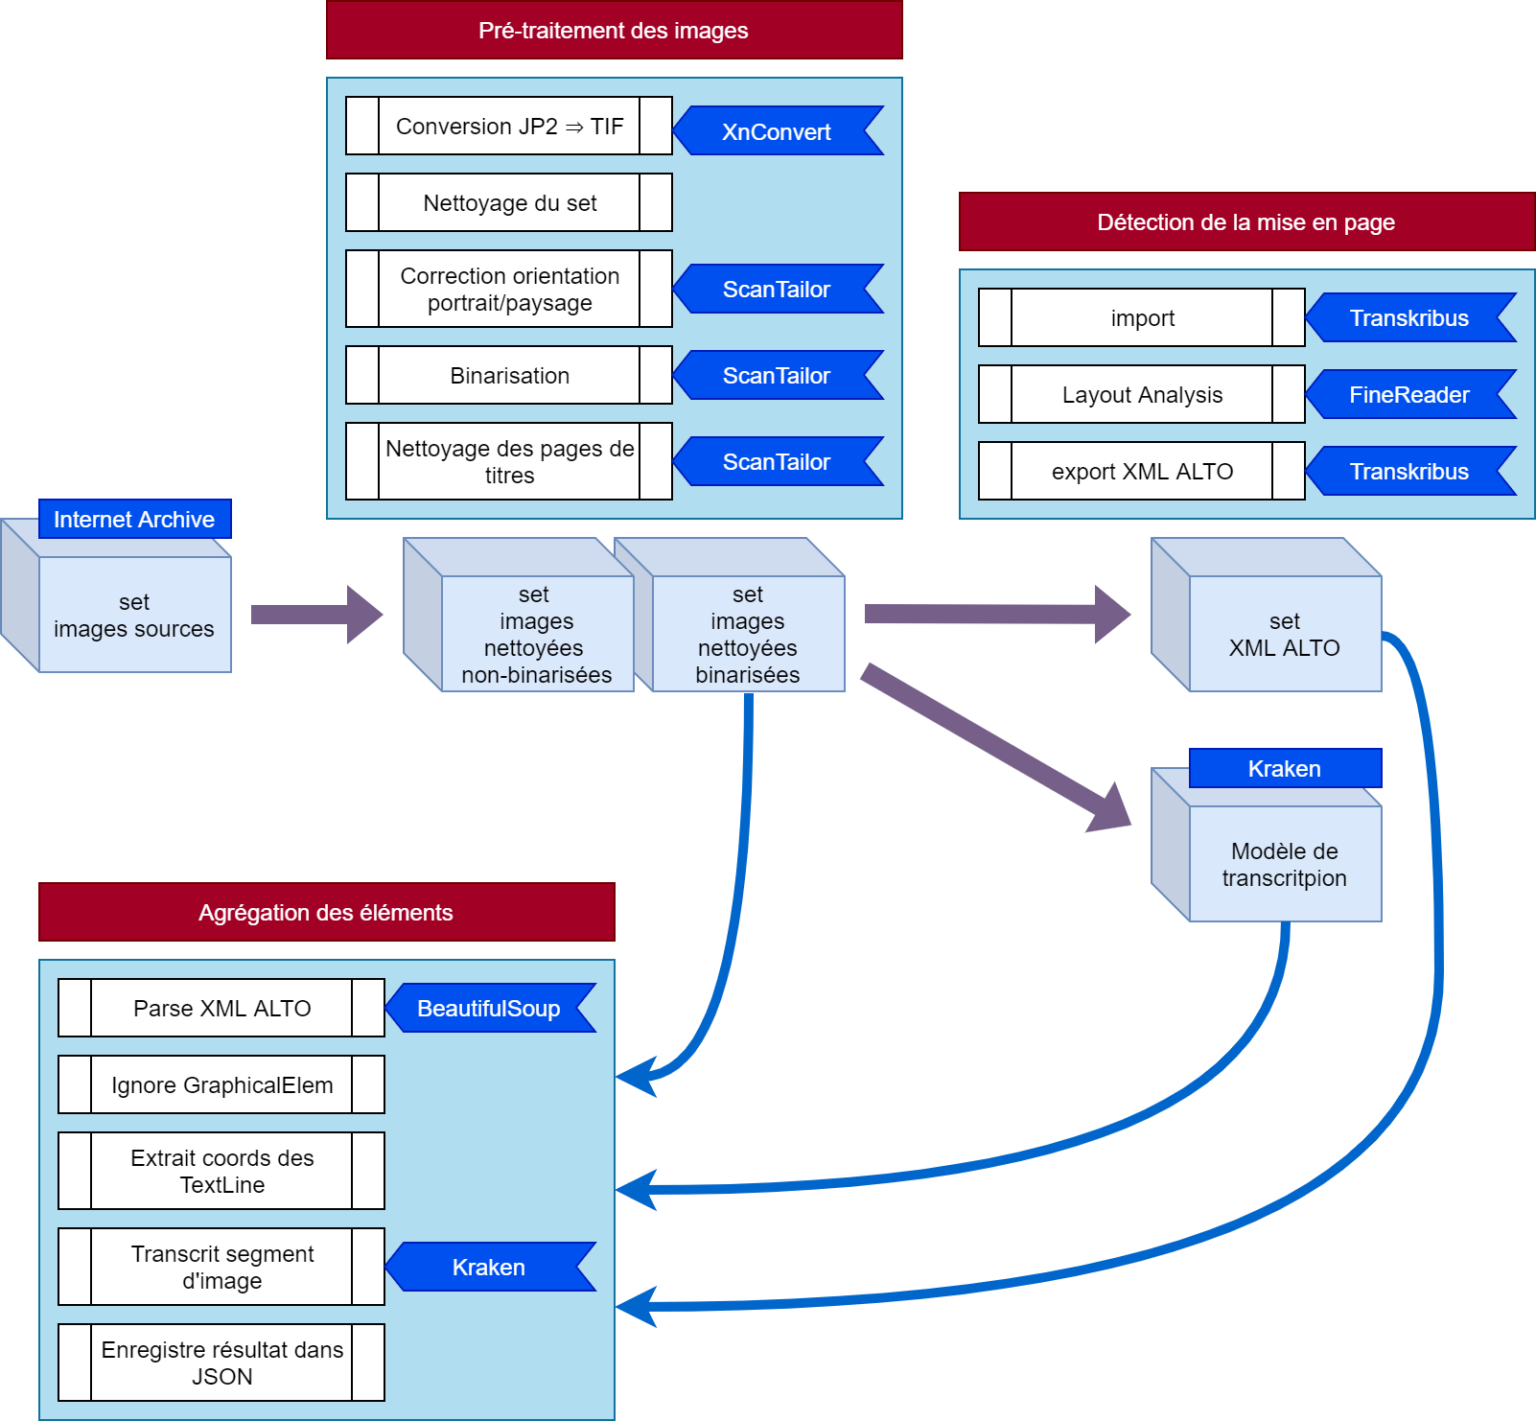
\includegraphics[width=15cm]{img/schema_lse_od2m.png}
    \caption[Schématisation des étapes suivies pour l’extraction du texte et des informations de mise en page]{Schématisation des étapes suivies pour l’extraction du texte et des informations de mise en page (source : Alix Chagué, \url{https://timeus.hypotheses.org/626}).}
    \label{fig:schema_lse_od2m}
\end{figure}

Dans le cadre du projet \timeus, étant donné les choix techniques déjà opérés pour le traitement des autres documents, deux solutions étaient envisageables pour la reconnaissance des caractères des \odm. La première était l'usage de \transkribus{}, la seconde utilisait \kraken{}.

\kraken{} est un logiciel libre développé en Python par Benjamin Kiessling\footnote{Chercheur du laboratoire d'humanités numériques \og Alexander von Humboldt \fg{} de l'Université de Leipzig (\textit{Leipzig  University’s  Alexander  von  Humboldt  Chair for Digital Humanities}). Benjamin Kiessling a également fait partie de l'équipe ALMAnaCH de 2018 à 2019.} à partir du système \textit{OCRopus}\footcite{kiessling}. Dans le processus d'\ocr, \kraken{} se passe de l'étape de la segmentation des mots et des caractères grâce à un \og réseau neuronal artificiel \fg{} qu'il utilise \og pour analyser l'image d'une ligne de texte, la séquence d'entrée, en une suite de caractères, la séquence de sortie \fg{}\footnote{\og \textit{[Kraken's] recognition engine operates as a segmentation-less sequence classifier using an artificial neural network to map an image of a single line of text, the input sequence, into a sequence of characters, the output sequence} : \cite{kiessling}.}. Ce point est l'apport principal de \kraken{} par rapport à tous les logiciels similaires tels que \transkribus{} : grâce à un apprentissage profond (\textit{deep learning}), il peut analyser un nombre important d'écritures de toute époque, latines et même arabes, et en proposer une transcription\footcite{kiesslingarabe}.

\og En 2018 \fg, note cependant Alix Chagué, \og il n’était pas possible d’obtenir une analyse de la mise en page complète avec \kraken \fg{}\footcite{chague2}. Mais le logiciel permettait déjà d'entraîner un modèle pour l'\ocr. Cela était également possible avec \transkribus, mais le fichier modèle ne peut pas être exporté depuis cette plate-forme, alors que l'opération est possible avec \kraken{}, qui donne de meilleurs résultats, sous la forme de fichiers \texttt{.mlmodel}. L'équipe ALMAnaCH a donc choisi de recourir à \kraken{} pour la phase de transcription (entraînement du modèle puis reconnaissance des caractères)\footcite{chague2}.

Les fichiers \og vérité terrain \fg{} étaient composés des transcriptions de 1300 lignes (fichiers texte) et de leurs images (fichiers image). Pour s'entraîner, \kraken{} itère sur chaque couple de fichiers, transcrit le fichier image et compare le résultat au contenu du fichier texte. Le passage en revue de l'ensemble des données (ici, les 1300 paires) constitue une \textit{epoch}. Un taux de réussite (\textit{accuracy report}) est calculé à la fin de chaque itération. Il se compose de trois données numériques : le taux de réussite (positif ou négatif), le nombre de caractères contenus dans l'\textit{epoch} et les faux-positifs (\cad{} le nombre de caractères mal reconnus). Plusieurs dizaines d'\textit{epochs} sont nécessaires pour parvenir à un taux de réussite optimal et donc à un modèle fiable (\fig{} \ref{fig:kraken_training}).

\begin{figure}
    \centering
    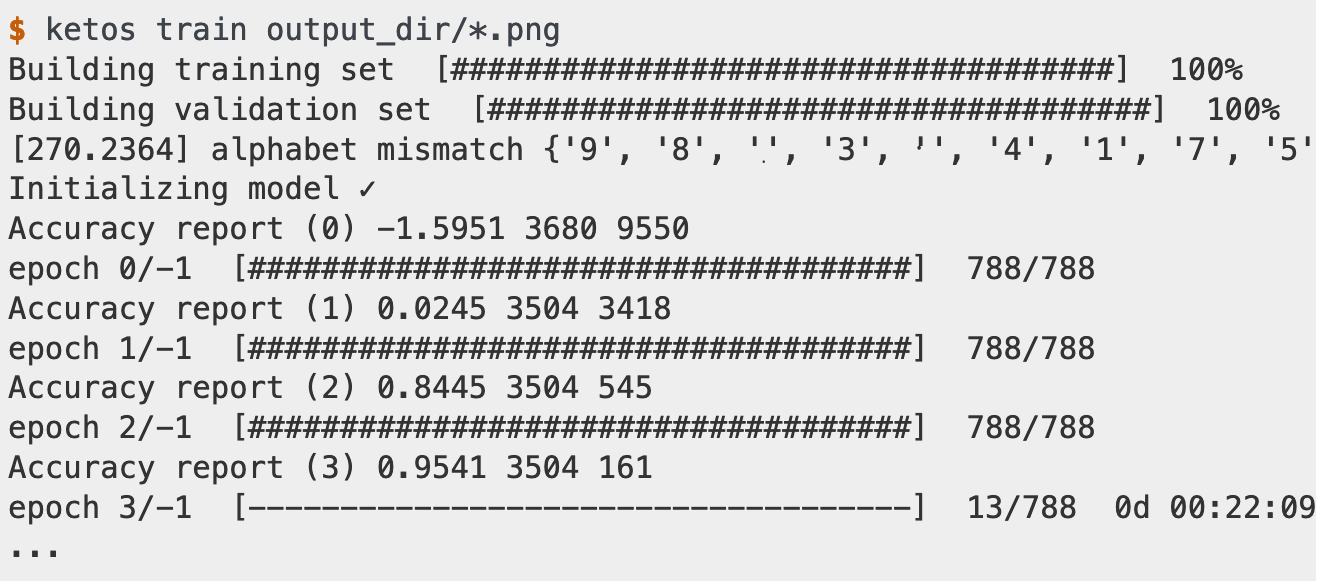
\includegraphics[width=15cm]{img/kraken_training.png}
    \caption[Exemple d'un entraînement opéré par \kraken]{Exemple d'un entraînement opéré par \kraken. Trois \textit{epochs} (\nos{}0 à 2) sont arrivées à leur terme, la quatrième étant en cours de chargement (\no{}3). Le taux de réussite augmente à chaque nouvelle \textit{epoch} : de \texttt{-1.5951} pour la première (\texttt{9550} fautes sur... \texttt{3680} caractères détectés), il atteint \texttt{0.8445} pour la troisième (\texttt{545} fautes sur \texttt{3504} caractères détectés). Capture d'écran du site de \kraken{} (\url{http://kraken.re/training.html}, consulté le \today).}
    \label{fig:kraken_training}
\end{figure}

Une fois ce modèle obtenu, la phase de transcription automatique pouvait commencer. \kraken{} pouvant être utilisé comme une librairie du langage Python, il a pu être envisagé de fédérer les étapes de transcription et d'encodage des textes obtenus sous l'égide d'un même script, \lse. Son fonctionnement débute ainsi :

\begin{enumerate}
    \item Il prend pour paramètres les fichiers images des \odm{} et les fichiers ALTO produit par \transkribus ;
    \item Chaque image est associé à son fichier ALTO ;
    \item Les coordonnées des lignes de texte sont extraits de l'ALTO et le script lance la transcription de ces lignes à l'aide de \kraken{} et du modèle précédemment obtenu.
    \item Les transcriptions de chacune des 6 608 images sont stockées dans autant de fichiers XML-TEI.
\end{enumerate}

Ces transcriptions relèvent du texte brut, \cad{} que la donnée n'y est pas structurée.

\subsection{Structuration}

C'est à ce stade que l'analyse de la structure logique menée précédemment est prise en compte (\ann{} \ref{structure}).

\begin{enumerate}
    \item Les limites des chapitres (monographies et éléments de paratexte) sont identifiées en fonction des pages de titres qui marquent le début de celui en cours et la fin du précédent.
    \item Les transcriptions sont rassemblées par chapitre.
    \item Si un chapitre est identifié comme étant une monographie, alors le script y lance une recherche pour détecter les titres de la structure logique. Le script est rendu tolérant par une distance de Levenshtein (ou distance d'édition) souple afin de reconnaître un titre en dépit d'une transcription partiellement fautive. La distance de Levenshtein mesure l'écart entre deux chaînes de caractères, ici entre le modèle (le titre standard) et sa transcription.
    \item Un arbre XML est créé en respectant les différents niveaux de la structure logique.
    \item En sortie, le script renvoie :
    \begin{itemize}
        \item Treize fichiers \og source \fg{} avec le contenu de chaque volume ;
        \item Deux cent vingt-trois fichiers correspondant à autant de chapitres détectés.
    \end{itemize}
\end{enumerate}

\section{Les fichiers XML-TEI}

Ces fichiers XML sont structurés avec un schéma TEI.

XML (\textit{Extensible Markup Language}, en français \textit{langage de balisage extensible}) est un format de données conçu pour la description des documents textuels, ne possédant pas de jeu de balises prédéfini\footnote{Définition d'Ariane Pinche : \url{https://github.com/ArianePinche/coursTNAH_XML-TEI/blob/master/seance01/InitiationXML.md} (consulté le \today).}.

La TEI (\textit{Text Encoding Initiative}) est un schéma de données XML commencé en 1987 dont le but est de \og fournir des recommandations pour la création et la gestion sous forme numérique de tout type de données créées et utilisées par les chercheurs en sciences humaines \fg\footcite[p. 9]{burnard}. Ses trois caractéristiques principales sont qu'il \og s’intéresse au sens du texte plutôt qu'à son apparence \fg, qu'il est \og indépendant de tout environnement logiciel particulier \fg{} et qu'il a été conçu par une communauté scientifique qui le maintient toujours aujourd'hui à travers le \textit{TEI Consortium} fondé en 2000\footcite[p. 9]{burnard}. 

Ce format conjugue ainsi une certaine \og flexibilité et un intérêt centré sur les besoins scientifiques \fg\footcite[p. 10]{burnard}. L'utiliser pour encoder les transcriptions des \odm, c'est donc décrire de la meilleure manière possible l'organisation originale du texte dans les volumes imprimés tout en assurant la pérennité de la donnée ainsi produite.

Un document XML peut être représenté sous une forme arborescente, \og l'arbre XML \fg{} (\fig{} \ref{fig:xmltree1}). Il débute par un élément racine (\texttt{<TEI>}) qui contient tous les autres.

Les trois grandes sections de l'arbre sont le \texttt{<teiHeader>}, les \texttt{<facsimile>} et le \texttt{<text>}. Le \texttt{<teiHeader>} est l'en-tête où se trouvent les métadonnées du document. Il est ici réduit à son minimum, n'étant composé que d'une description bibliographique (\texttt{<fileDesc>}) : le titre et ses auteurs (\texttt{<titleStmt>}), l'organisation responsable de la publication, la date et le lieu de celle-ci (\texttt{<publicationStmt>}), et enfin une description sommaire des \odm{} (\texttt{<sourceDesc>})\footnote{\og Les \odm{} sont des recueils d'enquêtes sociologiques publiées pendant la deuxième moitié du \textsc{xix}\ieme{} siècle. Ces enquêtes ont été rassemblées sous la forme de 3 séries de plusieurs volumes. Accès aux fichiers images sources : \url{http://timeusage.paris.inria.fr/mediawiki/index.php/Aperçu_des_états\#Les_Ouvriers_des_Mondes} \fg.}. L'en-tête contient également un \texttt{<encodingDesc>} où le lien est fait avec le programme ANR ; l'action du script \lse{} est également mentionnée\footnote{\og Cette édition numérique des \odm{} a été réalisée dans le cadre du projet ANR \timeus{} (\url{http://larhra.ish-lyon.cnrs.fr/anr-time-us}). Elle est générée automatiquement grâce au programme \lse{} (\url{https://gitlab.inria.fr/almanach/time-us/LSE-OD2M}), développé par Alix Chagué, équipe Inria ALAMAnaCH \fg.}.

\begin{figure}
    \centering
    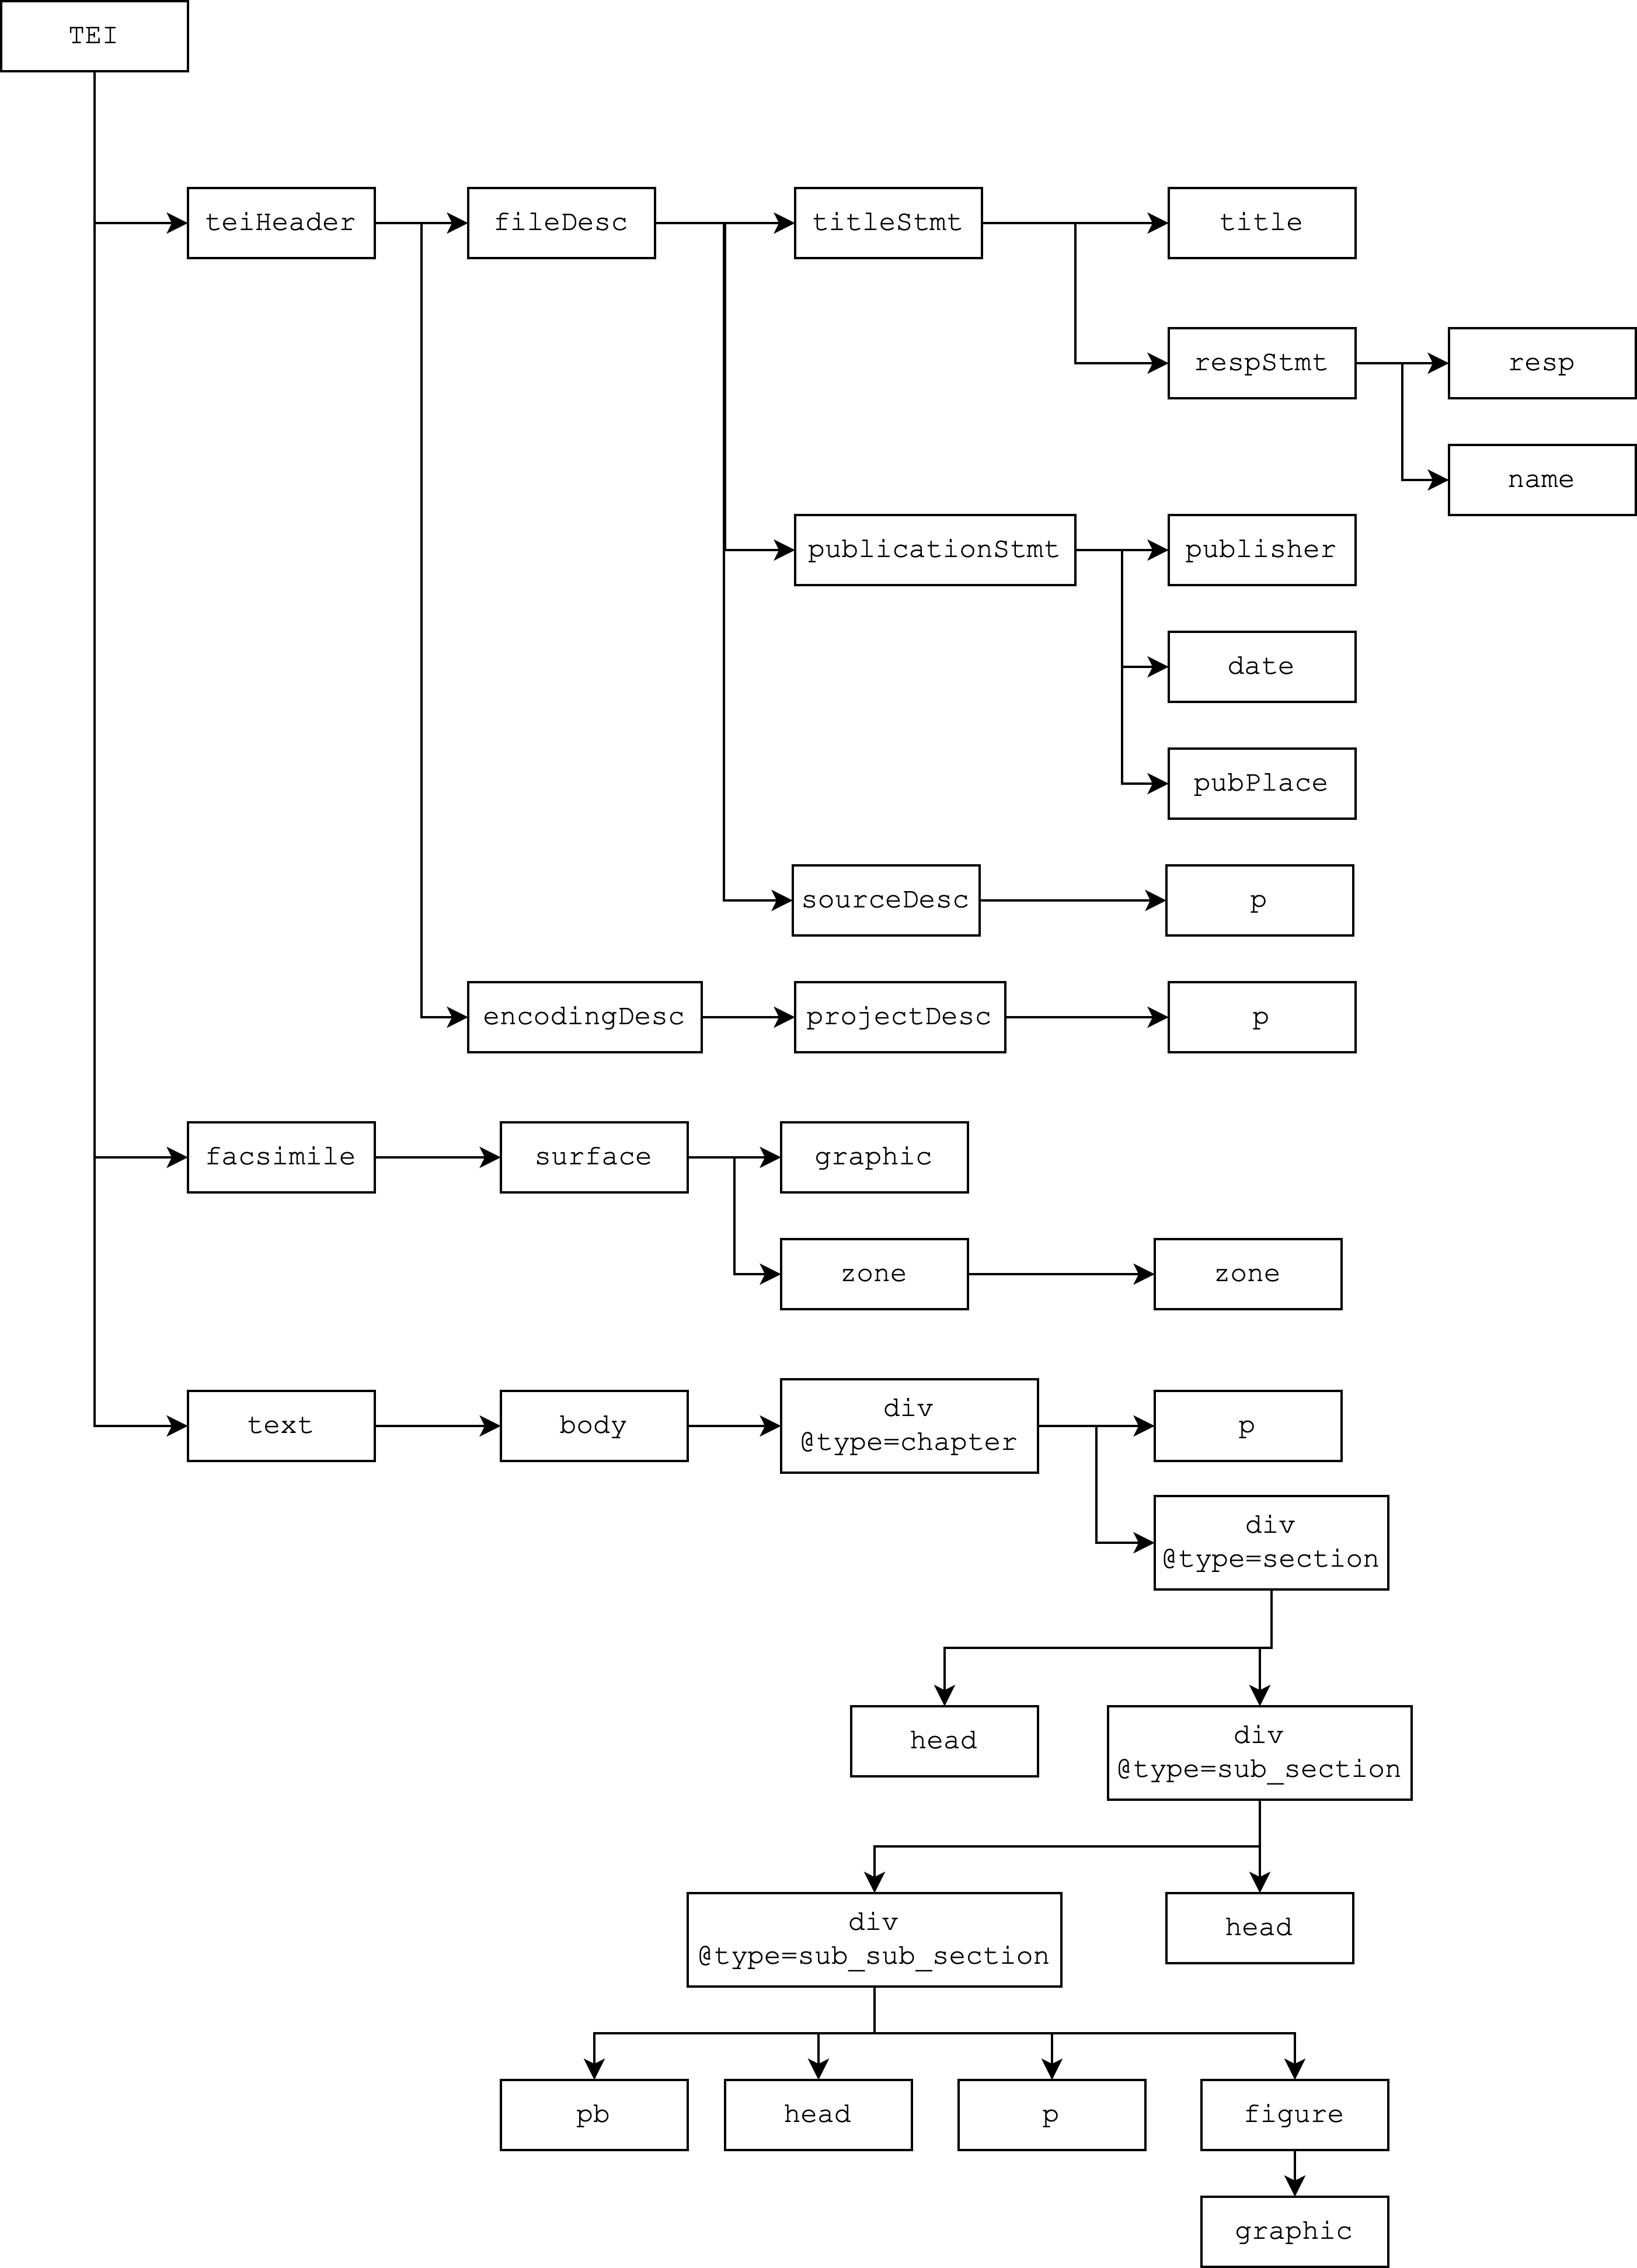
\includegraphics[width=16cm]{img/arbre_xml.png}
    \caption[Représentation de l'arbre XML des fichiers TEI]{Représentation de l'arbre XML utilisé par le script \lse{} pour encoder les transcriptions des monographies des \odm.}
    \label{fig:xmltree1}
\end{figure}

Le document continue avec une succession de balises \texttt{<facsimile>} dont le but est de conserver le lien entre le texte et son segment dans l'image d'origine (\fig{} \ref{fig:facsimile})\footnote{\textit{TEI Guidelines, 11 Representation of Primary Sources, 11.1 Digital Facsimiles} (\url{https://tei-c.org/release/doc/tei-p5-doc/fr/html/PH.html\#PHFAX}, consulté le \today).}. L'élément suivant, \texttt{<surface>}, possède quatre attributs : \texttt{@ulx} et \texttt{@uly} qui ont pour valeurs l'abscisse \textit{x} et l'ordonnée \textit{y} du coin supérieur gauche du bloc de segmentation (la page), et \texttt{@urx} et \texttt{@ury} contenant les valeurs de l'abscisse \textit{x} et de l'ordonnée \textit{y} du coin inférieur droit. Ces coordonnées sont directement reprises des fichiers XML ALTO obtenus avec \textit{FineReader}. On trouve ensuite un élément \texttt{<graphic>} avec un attribut \texttt{@url} ayant pour valeur le chemin local vers l'image de la page, et un élément \texttt{<zone>} contenant lui-même un ensemble de balises \texttt{<zone>}. Ces dernières contiennent les coordonnées des blocs de segmentation à l'intérieur du bloc supérieur définit par \texttt{<surface>} ; ces sous-blocs sont catégorisés par un attribut \texttt{@rendition} ayant pour valeur \texttt{paragraph} lorsqu'il s'agit de texte ou \texttt{table} pour un tableau.

\begin{figure}
    \centering
    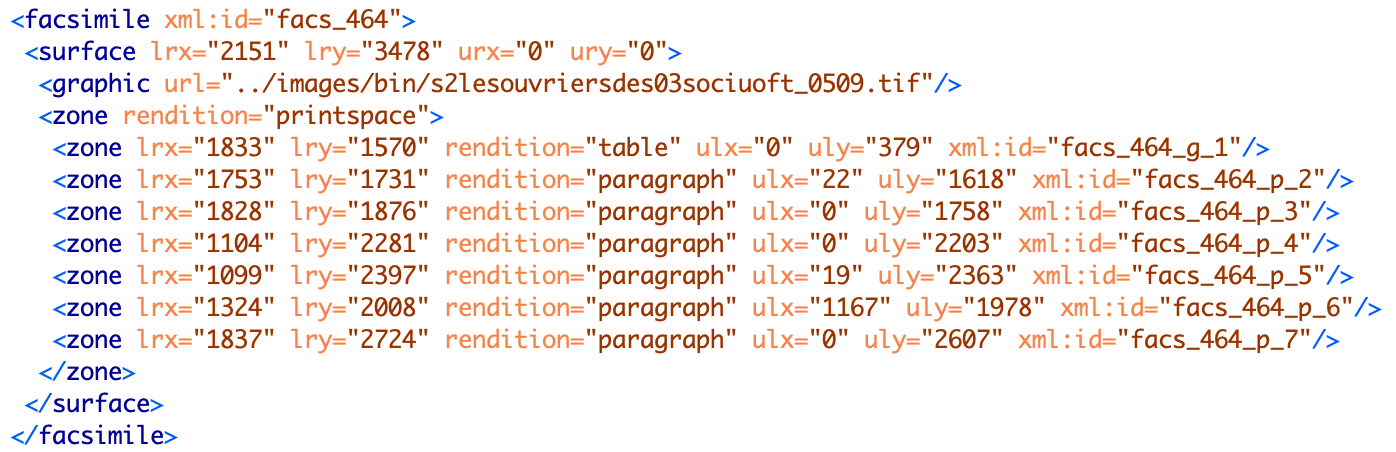
\includegraphics[width=16cm]{img/facsimile.png}
    \caption[Exemple d'un ensemble \texttt{<facsimile>}]{Exemple d'un ensemble \texttt{<facsimile>} dans le fichier source du troisième volume de la deuxième série.}
    \label{fig:facsimile}
\end{figure}

Le \texttt{<teiHeader>} et les éléments \texttt{<facsimile>} montrent que la structuration d'un texte brut issu d'une \ocr{} ne consiste pas simplement en l'encodage de la transcription. Il s'agit aussi de produire des métadonnées permettant de décrire le contenu du fichier.

La dernière section de l'arbre, \texttt{<text>}, contient les transcriptions structurées au sein de son élément \texttt{<body>}. Notons que l'implémentation de la structure logique par \lse{} n'a pas donné de résultats optimaux et a fait l'objet d'une reprise majeure lors du stage. Ces résultats restent néanmoins satisfaisants au regard du temps alloué pour l'écriture et le fonctionnement du  script (trois mois). 

Le principe retenu est le suivant : chaque division de la structure est enchâssée dans un élément \texttt{<div>} pour lequel un attribut \texttt{@type} vient préciser son niveau. De manière assez classique, cet encodage traduit ainsi la hiérarchie sémantique interne aux monographie grâce à une imbrication de \texttt{<div>} jusqu'à arriver au texte lui-même\footcite[p. 117]{clerice}. Les valeurs de l'attribut \texttt{@type} sont calquées sur les divisions des documents du langage de composition \LaTeX{} : \texttt{\textbackslash chapter\{\}}, \texttt{\textbackslash section\{\}}, \texttt{\textbackslash subsection\{\}}, \texttt{\textbackslash subsubsection\{\}}. Cela a pour but de faciliter une éventuelle transformation des documents XML-TEI au format \LaTeX\footcite[p. 52]{chague2}.

La monographie correspond à une \texttt{<div>} de type \texttt{chapter}. Les ensembles de niveau~A (page de titre, \textit{Observations préliminaires} et \textit{Notes}) sont de type \texttt{section}, les titres de niveau~I \texttt{sub\_section} et les paragraphes \texttt{sub\_sub\_section} (\textit{cf.} \ann{} \ref{structure}). Dans chaque niveau, le titre en lui-même est encodé au sein d'un élément \texttt{<head>}, le texte se trouvant ensuite dans des \texttt{<p>} (\fig{} \ref{fig:ex_structure}).

Pour les éléments de paratexte, tels que les avertissements liminaires de chaque volume, seul le niveau \texttt{chapter} a été utilisé, l'ensemble du texte se trouvant dans des \texttt{<p>}.

\begin{figure}[t]
    \centering
    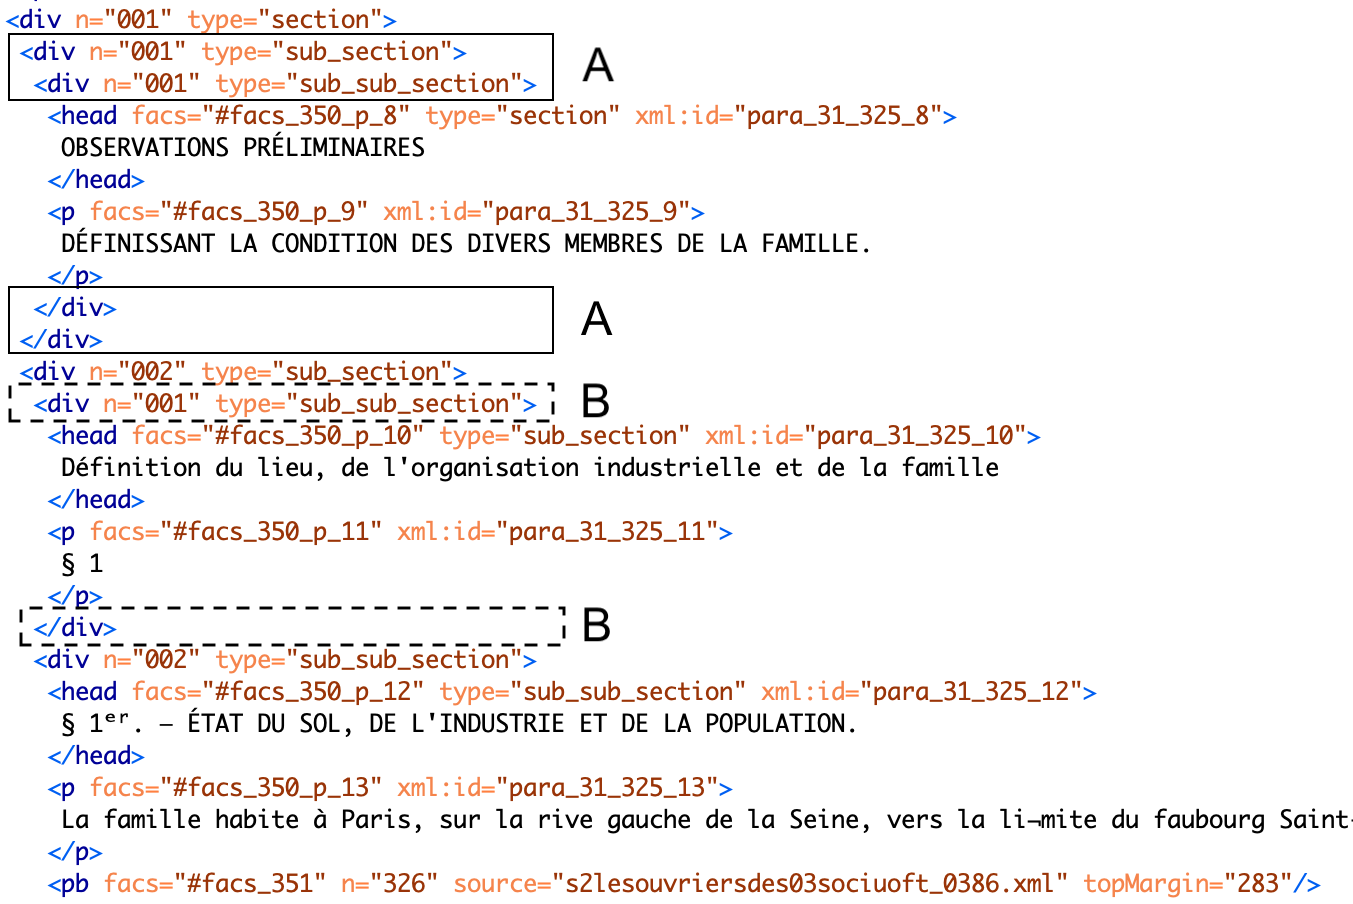
\includegraphics[width=16cm]{img/ex_structure.png}
    \caption[Exemple de la structuration du début de la monographie \no{}70]{Exemple de la structuration du début des \textit{Observations préliminaires} de la monographie \no{}70 par le script \lse{} (\texttt{s2t3\_chapt\_31.xml}). L'encodage est fautif dans la mesure où des niveaux supplémentaires ont été rajoutés : \textit{Observations...} ne devrait être que dans une \texttt{section} (les lignes des repères A n'ont pas lieu d'être), \textit{Définitions du lieu...} dans une \texttt{sub\_section} (les lignes des repères B sont fautives). On remarque également une erreur de transcription, le numéro de paragraphe (§1) étant répété. La balise finale, \texttt{<pb>}, marque un changement de page.}
    \label{fig:ex_structure}
\end{figure}

Le script \lse{} a été lancé sur le \textit{cluster} (ou \textit{grappe de serveurs}) \rioc{} d'Inria, où il a fallu un peu plus de quinze heures pour traiter l'ensemble des fichiers. Un \textit{cluster} est un groupe d'ordinateurs inter-connectés où une \og reine \fg{} (le \textit{master node}) répartit grâce à un \og planificateur \fg{} (\textit{scheduler}) les tâches qui lui sont demandées à des \og ouvrières \fg{} (les \textit{slave nodes})\footnote{\textit{\rioc{} Architecture}, \url{https://sed-paris.gitlabpages.inria.fr/rioc/rioc_architecture/rioc_architecture.html} (consulté le \today).}. Quatre des \og ouvrières \fg{} de \rioc{} possèdent des GPU (\textit{graphics processing unit}). Équipées d'une carte graphique, ces processeurs sont capables de réaliser du calcul vectoriel et peuvent ainsi traiter les images --- par exemple les pages des \odm{} --- très rapidement. Cette architecture en réseau permet d'augmenter de façon significative la vitesse de calcul et donc l'exécution des tâches.

Au final, les treize fichiers source créés par \lse{} représentent 25,5 Mo. Ils ont été divisés en 223 fichiers (25,7 Mo) nommés de la façon suivante : \texttt{s[numéro de la série]t[numéro du volume]\_chapt\_[numéro du chapitre].xml} (\ann{} \ref{mapping}).

\clearpage

\vspace*{\stretch{0.3}}

Au moment de commencer notre stage, nous avons donc trouvé un ensemble de 223 fichiers XML contenant les transcriptions structurées avec un schéma TEI des treize volumes des \odm. Les fichiers contenaient des enquêtes sociologiques (les monographies) et des éléments de paratexte. Les chercheurs et les chercheuses du programme ANR \timeus{} n'étaient intéressés que par les monographies, mais Inria avait la volonté de valoriser l'ensemble des fichiers.

Plusieurs points avaient été identifiés comme posant problème pour une future valorisation sous la forme d'une publication ou d'une réutilisation dans des projets de traitement automatique du langage (TAL).

Nous allons à présent exposer les différentes reprises que nous avons menées.
\vspace*{\stretch{1.7}}

\newpage
\thispagestyle{empty}
\mbox{}
\newpage
\cleardoublepage
\part{Une structuration à reprendre}

\clearpage
\thispagestyle{empty}
\cleardoublepage

\chapter{Outils, méthodologie et gestion du projet}


\section{Outils de développement}

\subsection{\gitlab}

La gestion quotidienne du programme \timeus{} se fait grâce à un dépôt sur \gitlab{}, un logiciel libre permettant aux entités comme Inria de créer une plate-forme interne de développement informatique. Sur \gitlab{} se trouve le dépôt central, organisé en plusieurs dossier. La technologie \textit{git} permet d'administrer les différentes versions du projet, sur une échelle à la fois verticale (les anciennes versions, appelées \commits, restant accessibles à travers un historique) et horizontale (le travail peut s'effectuer sur des \textit{branches} divergentes de la branche principale dite \master{} sans affecter l'état de cette dernière). Un commentaire est ajouté par l'utilisateur à chacun de ses \commits{} pour résumer ses modifications.

Chaque participant peut rapatrier le dépôt \gitlab{} en local pour travailler dessus ; ce rapatriement est un \textit{pull}. Il peut ensuite effectuer l'opération inverse, un \textit{push}, consistant à mettre ses \commits{} en ligne. Son équipe peut ainsi prendre connaissance des dernières avancées de la branche sur laquelle il travaille.

Une fois le travail dans une branche achevé, celle-ci peut être fusionnée avec \master. \gitlab{} propose une interface pour effectuer des \mergerequests{}. Il s'agit d'une demande de fusion, où \gitlab{} affiche l'historique de la branche. Les utilisateurs peuvent ainsi contrôler l'ensemble des \commits{} de la branche locale et vérifier qu'ils ne vont pas corrompre \master{} en créant des conflits (\textit{merge conflicts}).

\gitlab{} permet enfin à ses utilisateurs d'exposer un élément posant problème, d'effectuer des suggestions ou encore de porter à l'attention de leur équipe une ressource utile à travers des \issues{} (ou \textit{tickets}). Les \issues{} et les \mergerequests{} sont numérotées (\texttt{\#\textbackslash d} et \texttt{!\textbackslash d}\footnote{Par exemple, \texttt{\#5} fait référence à la cinquième \issue{} et \texttt{!5} à la cinquième \mergerequest{}.}), écrire leurs numéros dans \gitlab{} ou dans le commentaire de modification d'un \commit{} permettant de faire automatiquement référence à elles à travers un lien interne.

L'équipe ALMAnaCH possède un espace sur la plate-forme \gitlab{} d'Inria, où un dossier (en accès restreint) est réservé au programme \timeus{}. C'est ici, dans un sous-ensemble, que se trouve le dépôt des \odm. Le script \lse{} est déposé dans un dossier externe.

La branche \master{} compte quatre sous-dossiers :

\begin{itemize}
    \item \texttt{source} contient les treize fichiers XML-TEI des volumes des \odm{} ;
    \item \texttt{script} contient les scripts développés afin d'automatiser le traitement des fichiers ;
    \item \texttt{files} contient les fichiers XML-TEI générés à partir des fichiers sources et modifiés automatiquement ou à la main en vue de leur publication (monographies et fichiers de paratexte) ;
    \item \texttt{metadata} contient des fichiers de métadonnées sur le projet.
\end{itemize}

Ce dossier était notre espace de travail principal, notre première action ayant consisté en son rapatriement au niveau local. Notre méthodologie était la suivante :

\begin{enumerate}
    \item Une branche était créée pour chaque mission ;
    \item Des \commits{} étaient effectués en local sur cette branche ;
    \item Les \commits{} d'une journée étaient mis en ligne sur \gitlab{} par un \textit{push} ;
    \item Lorsque la mission était achevée, une \mergerequest{} était ouverte ;
    \item La \mergerequest{} était acceptée et la branche fusionnée avec \master.
\end{enumerate}

\begin{figure}
    \centering
    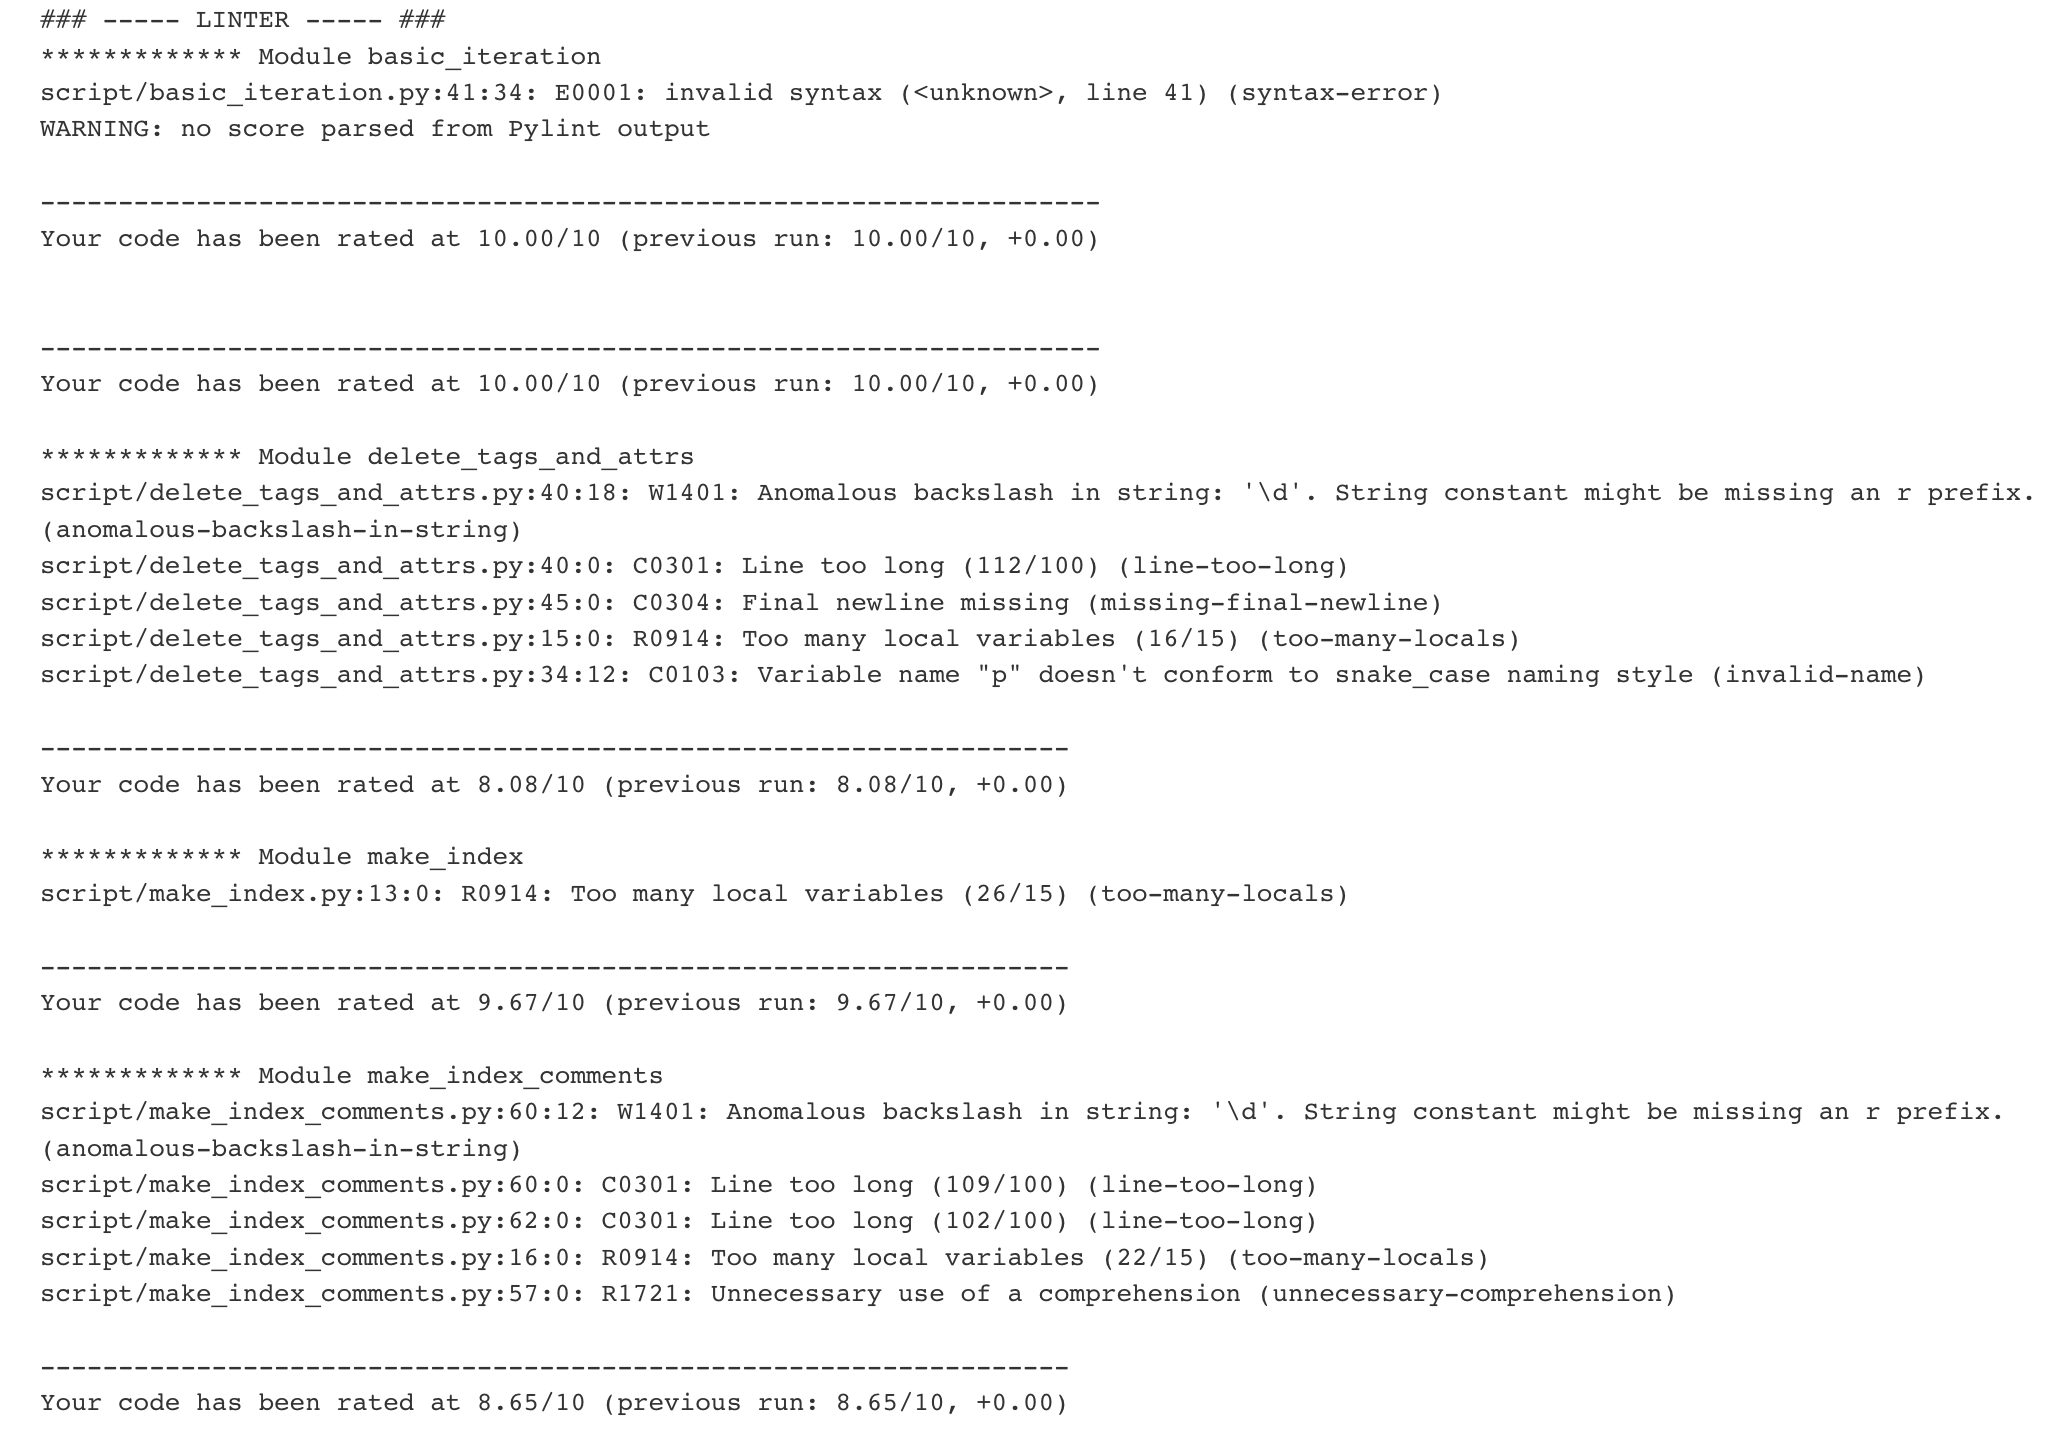
\includegraphics[width=15cm]{img/pylint_output.png}
    \caption[Exemple d'un contrôle de code par \textit{Pylint}]{Exemple d'un contrôle de code par \textit{Pylint}, qui donne une note à chaque script (\textit{module}) et détaille ensuite les erreurs détectées.}
    \label{fig:pylint}
\end{figure}

Le \textit{linter} \textit{Pylint} était également implanté dans le dépôt ; il s'agit d'un système de vérification de code Python. Son rôle est de contrôler à chaque \textit{push} la qualité du code des scripts, notamment la longueur des lignes, les intitulés des variables ou encore la documentation des fonctions. Le résultat est affiché dans une console sous forme de messages désignant le fichier concerné, la ligne de l'erreur et une désignation standardisée de celle-ci (\textit{line too long}, \textit{final newline missing}, etc. : \fig{} \ref{fig:pylint}).

\subsection{\pycharm{} et \oxygen}

Pour manipuler les fichiers XML, développer et activer les scripts Python, nous usions des logiciels \oxygen{} (éditeur de code XML sous licence propriétaire) et \pycharm{} (environnement de développement intégré pour la programmation en Python, une version est sous licence libre et une seconde sous licence propriétaire). 

Plusieurs fonctionnalités d'\oxygen{} ont facilité le traitement du corpus, notamment la possibilité de rassembler l'ensemble des fichiers dans un \og projet \fg. Par ce biais, des opérations --- par exemple effectuer une recherche ou remplacer une expression par une autre --- peuvent être menées sur le corpus sans requérir l'ouverture successive de chaque fichier. En outre, le logiciel dispose d'un système de validation du schéma du code, qui là encore peut être appliqué à tout le corpus à travers l'outil \og projet \fg.

\pycharm{} est équipé d'un outil de type \textit{linter} comparable à \textit{Pylint}, qui permet de s'assurer de la validité et de la lisibilité du code et facilite la programmation. \textit{Pylint} est cependant plus exigeant que le \textit{linter} natif de \pycharm, un double contrôle était donc nécessaire.

\section{Espaces de discussion}

La situation de confinement d'avril à mai et le maintien de la fermeture aux stagiaires des locaux d'Inria de juin à juillet a conduit à la mise en place d'outils de discussion.

\subsection{\Mattermost}

\Mattermost{} est un logiciel de discussion instantanée dont le code, écrit à l'origine sous un format propriétaire, a été publié en \opensource{}\footnote{Consultable sur \github{} (\url{https://github.com/mattermost/mattermost-server}, consulté le \today).} en 2015\footnote{Lindsay Brock, \textit{Open source Slack-alternative reaches 1.0: Self-host ready, Slack-compatible, MIT licensed}, 2 octobre 2015, \url{https://mattermost.com/blog/mattermost-3-4-16/} (consulté le \today).}. Auto-hébergé --- Inria stocke le code dans ses propres installations et n'a pas recours à un serveur distant ---, il s'agit de l'espace de discussion principal des agents d'Inria.

Composé de plusieurs \og chaînes \fg{} (\textit{public channels}) organisées de façon thématique, il leur permet d'échanger sur les différents projets et de suivre leur avancement, mais aussi d'exposer les difficultés techniques qu'ils rencontrent dans leur travail quotidien afin d'obtenir de l'aide. La chaîne \og \ocr \fg{} est ainsi fréquemment utilisée par les utilisateurs de \kraken{} (\fig{} \ref{fig:mattermost}).

\begin{figure}
    \centering
    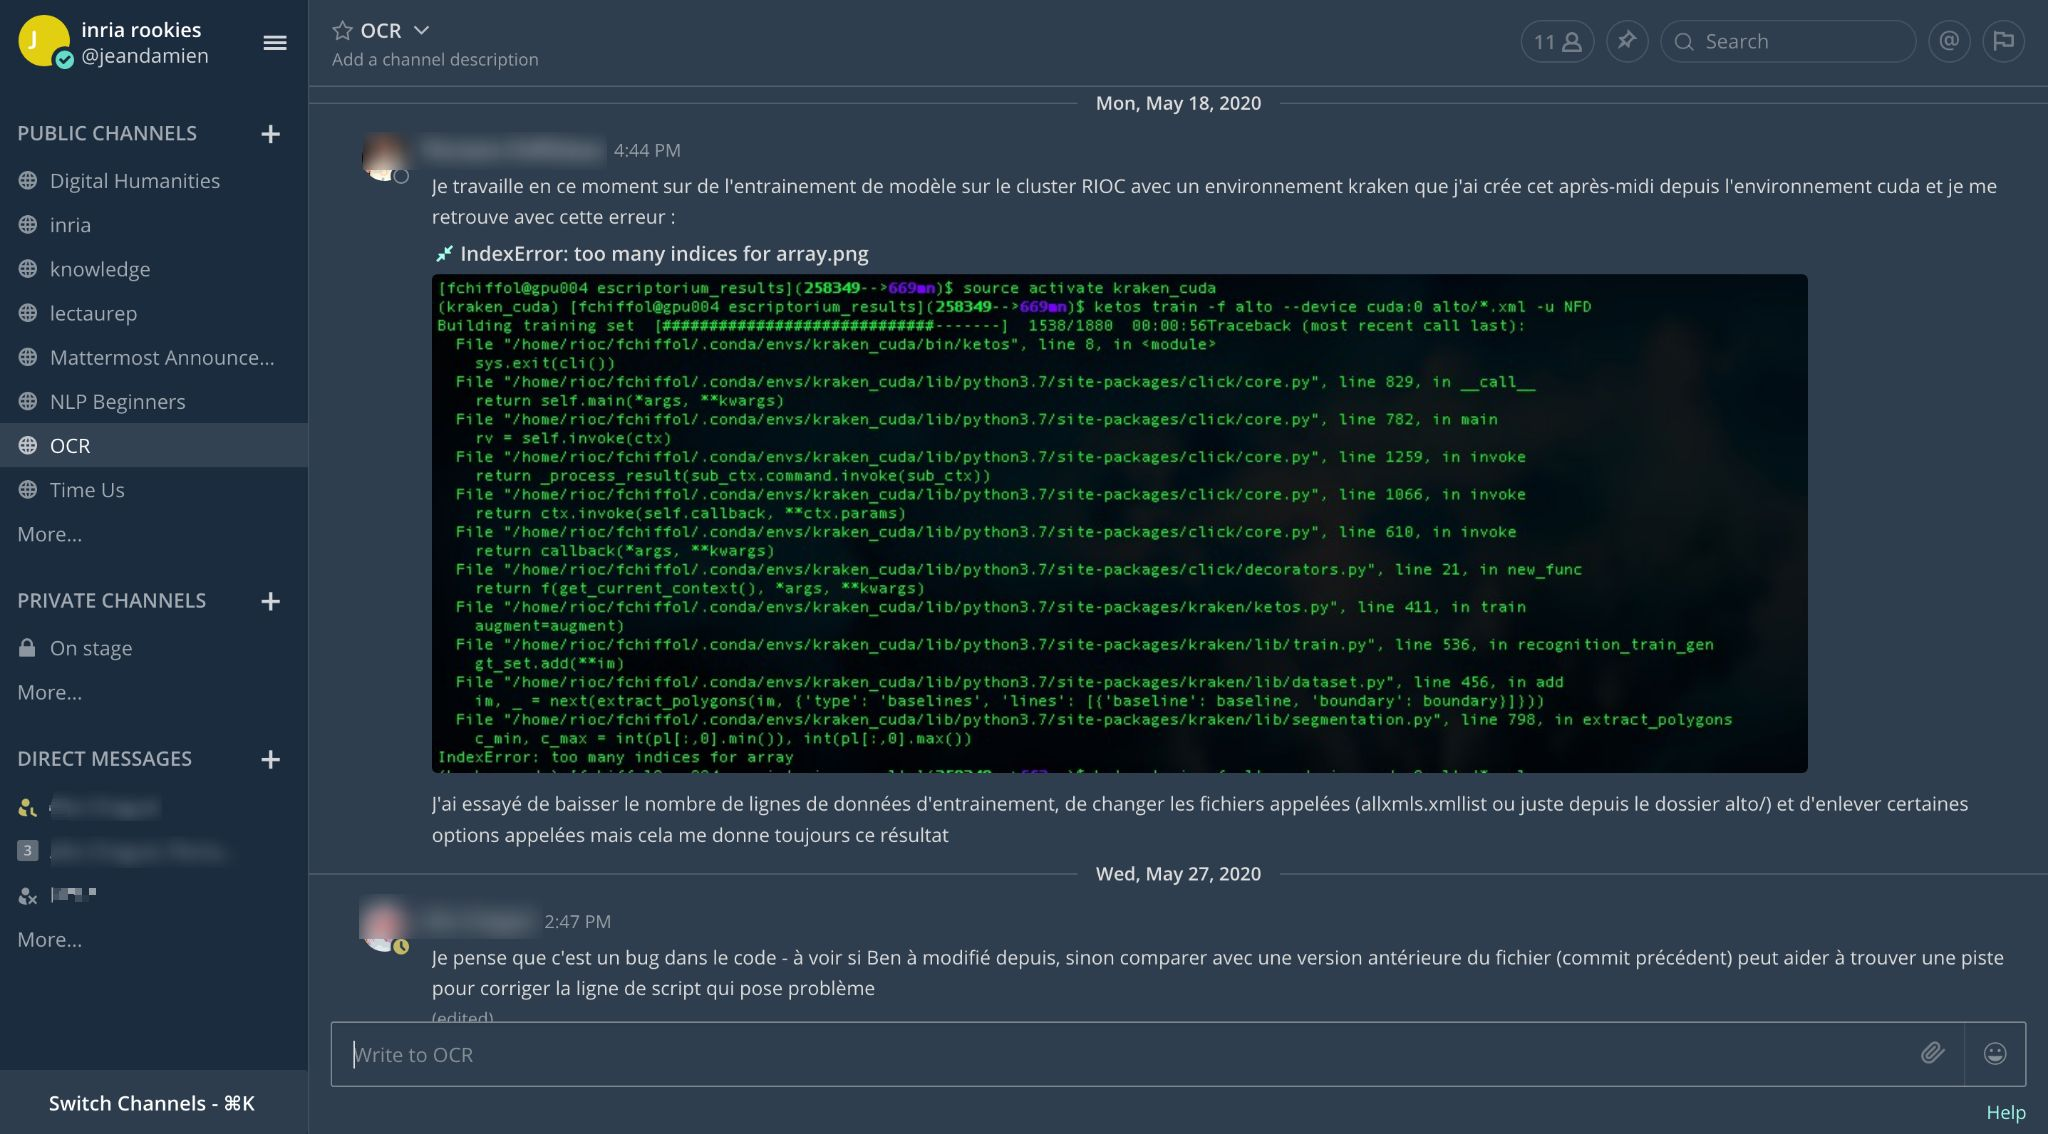
\includegraphics[width=16cm]{img/mattermost.jpg}
    \caption[\Mattermost{}]{Exemple de messages sur la chaîne \og \ocr \fg{} du \Mattermost{} d'Inria : une utilisatrice demande de l'aide au sujet d'une erreur dans l'exécution de \kraken{}. Sur le volet gauche se trouve la liste des chaînes disponibles.}
    \label{fig:mattermost}
\end{figure}

\subsection{\textit{Issues} et \mergerequests{} sur \gitlab}

Le programme \timeus{} possède également une chaîne ; cependant, pour les échanges afférents à nos missions, nous usions des espaces de discussion de \gitlab.

Les \issues{} et les \mergerequests{} n'ont en effet pas pour seule utilité de permettre aux utilisateurs d'exposer des problèmes ou de demander des fusions de branches. Il s'agit d'espaces dynamiques qui participent pleinement à la gestion de projet en offrant à ses participants la possibilité de donner leur avis ou d'apporter des solutions, par exemple pour résoudre un \textit{merge conflict}.

Cet aspect est facilité par l'usage du langage à balises \markdown\footnote{\gitlab{} use de sa propre version du \markdown, le \textit{GitLab Flavored Markdown} : \url{https://docs.gitlab.com/ee/user/markdown.html} (consulté le \today).}. Il permet une mise en forme légère (listes, liens hypertexte, diagrammes), ainsi qu'une intégration d'échantillons de code. Si ceux-ci ne sont pas fonctionnels, le \markdown{} permet de leur appliquer une coloration syntaxique, les rendant ainsi plus facile à lire (\fig{} \ref{fig:ex_gitlab}).

Les échanges sur ces espaces restent accessibles après la clôture des \issues{} ou des \mergerequests{}, constituant ainsi un historique de l'avancement du projet.

\begin{figure}
    \centering
    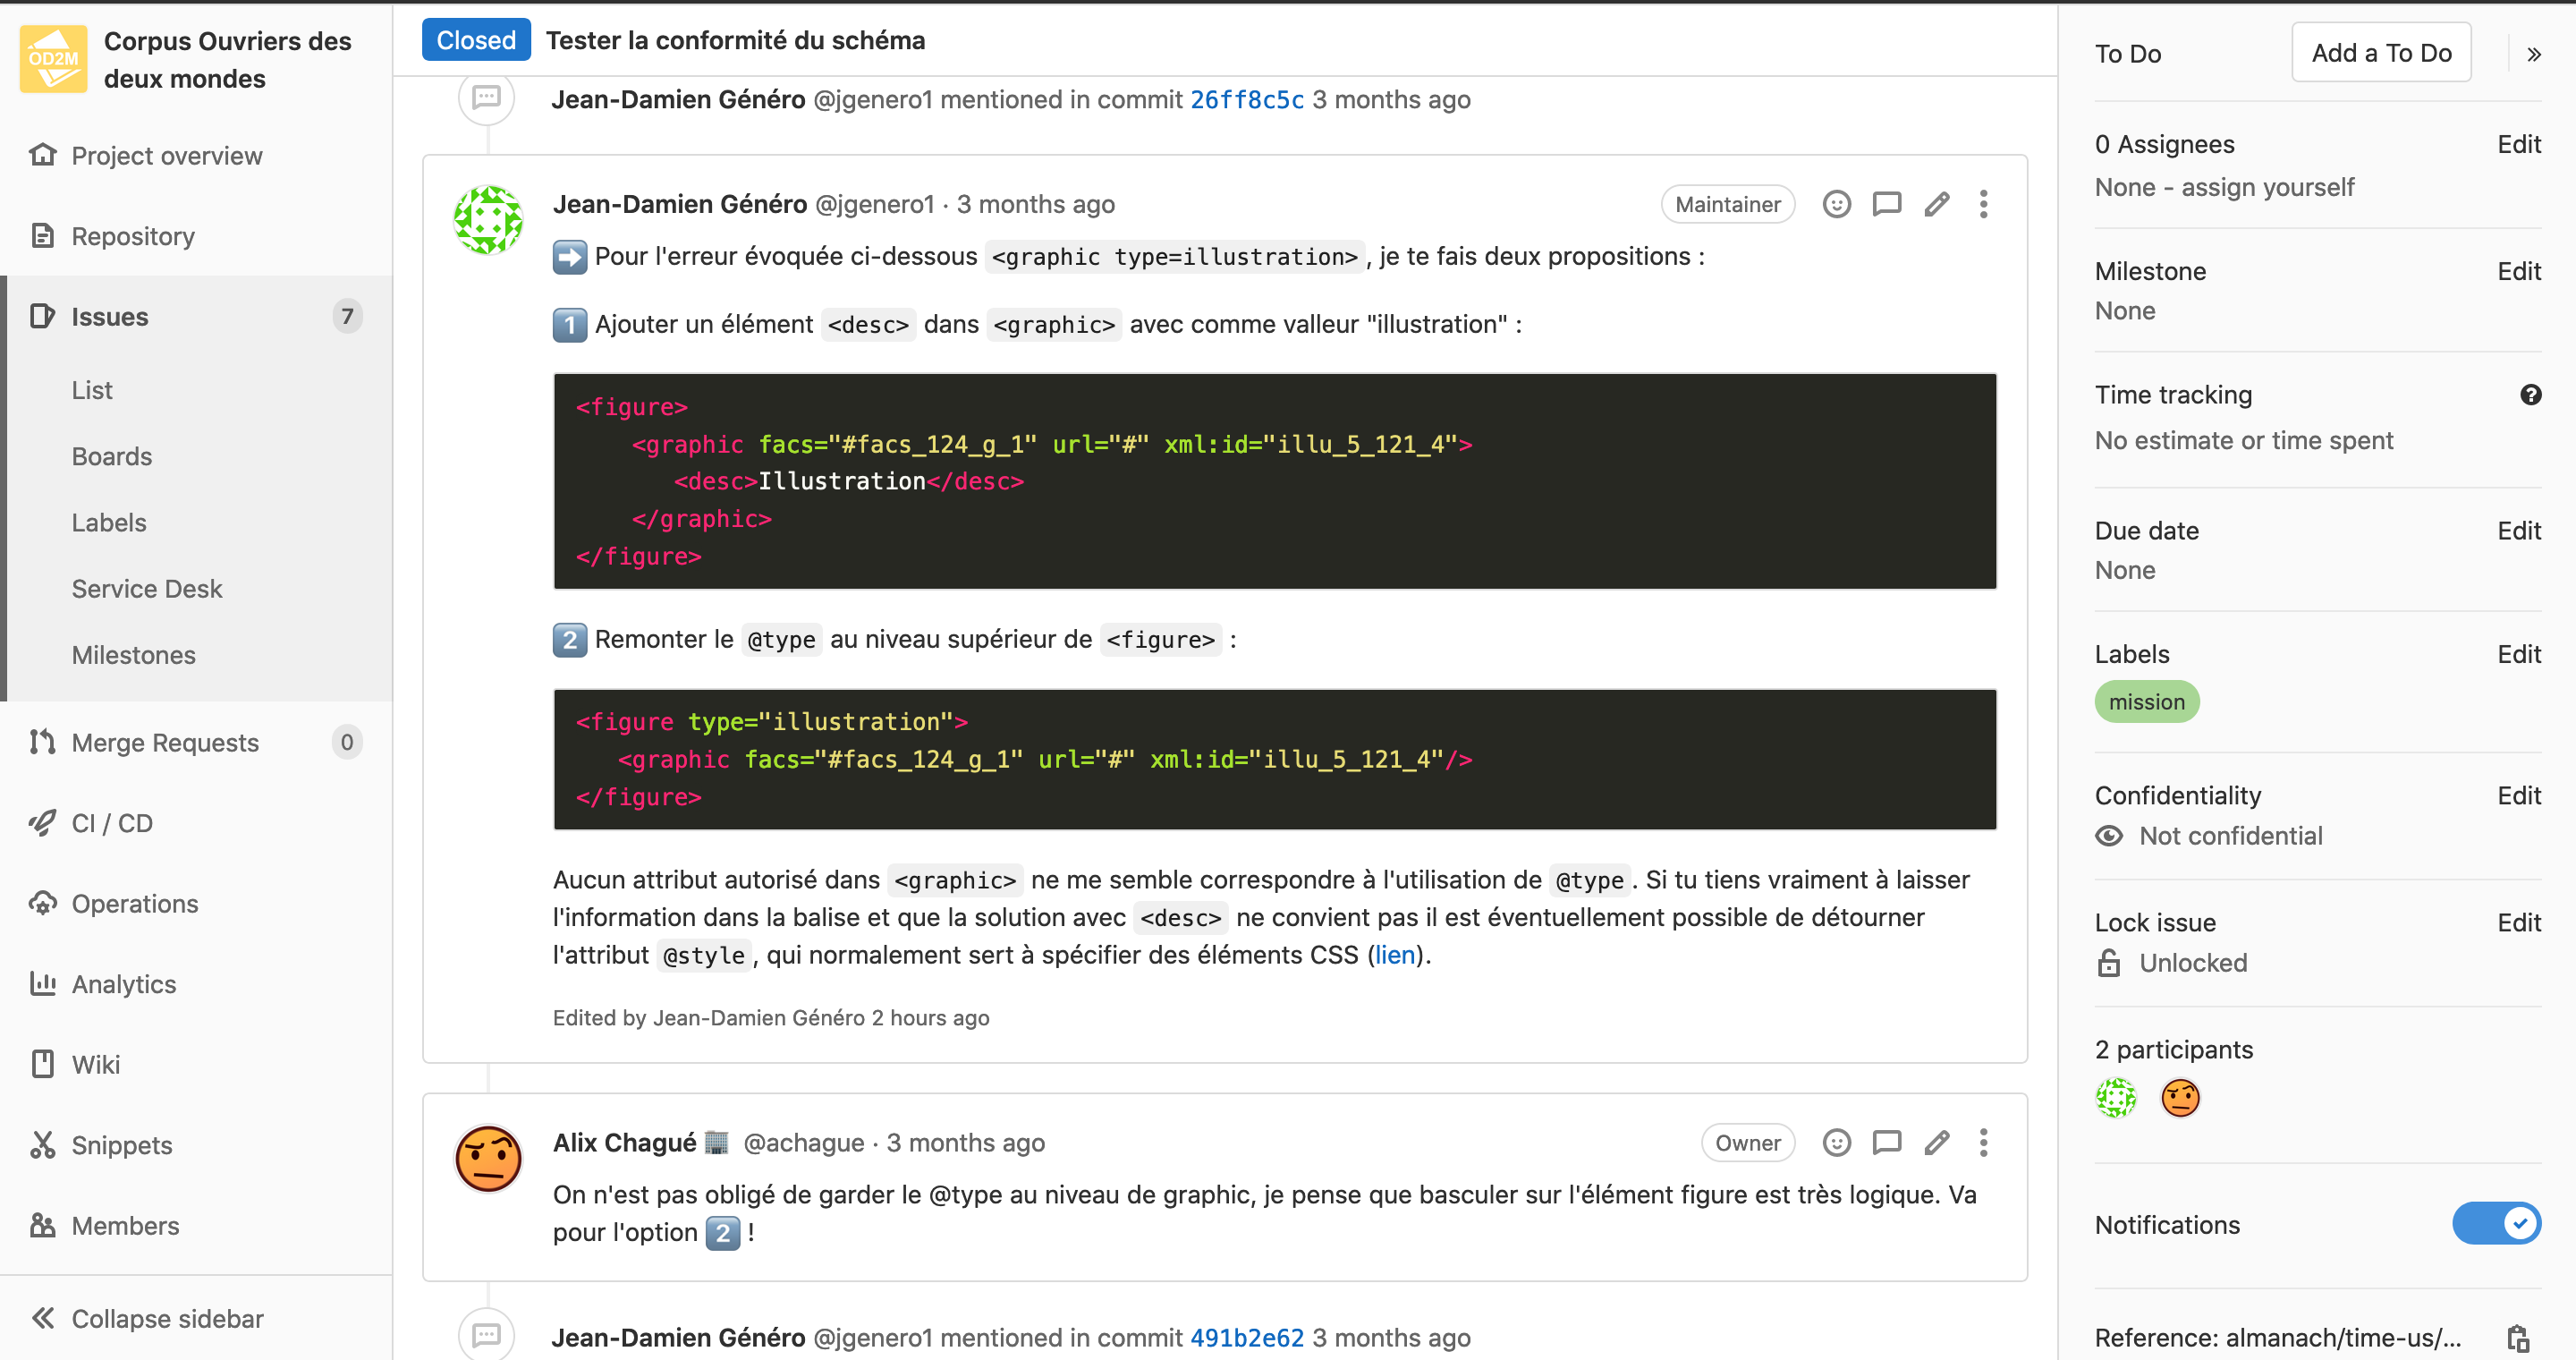
\includegraphics[width=16cm]{img/gitlab.png}
    \caption[Messages dans une \issue{} \gitlab]{Exemple de messages échangés avec une coloration syntaxique d'un code Python dans une \issue{} sur \gitlab.}
    \label{fig:ex_gitlab}
\end{figure}

\section{Feuille de route}

\subsection{Les missions du stage}

Au commencement de notre stage, huit \issues{} étaient ouvertes sur le \gitlab{} des \odm{}. Chacune correspondait à un problème ou à un point qui n'avait pas encore pu être développé. Elles constituaient donc notre \og feuille de route \fg, \cad{} l'exposé des missions que nous avions à réaliser (\ann{} \ref{ann:feuille_route}). Il nous a été demandé de les utiliser pour poser nos questions ou proposer nos solutions.

Les missions qui nous ont été confiées étaient de deux ordres.

Une première moitié consistait à contrôler les résultats du script \lse, tant au niveau du corpus qu'à celui de chaque fichier, et à effectuer des reprises si nécessaire. Tout d'abord, il s'agissait de détecter les erreurs de découpage des fichiers de volume et d'opérer les fusions ou les séparations nécessaires. Ceci avait pour but de donner à chaque fichier un identifiant unique après s'être assuré de l'unité de son contenu (\issue{}~1). Dans un second temps, nous devions nous intéresser à des éléments particuliers dans chaque fichier, à l'instar du contenu des balises \texttt{<facsimile>} (\issue{}~2), de la qualité des transcriptions (\issue{}~6) ou encore de la validité du schéma TEI (\issue{}~3); le contrôle de l'implémentation de la structure logique ayant constitué notre occupation principale.

L'autre moitié de nos missions avait pour but de valoriser les données des \odm{} en menant des actions ciblées. La principale consistait à identifier les individus enquêtés en liant les informations onomastiques du deuxième paragraphe (\textit{État civil de la famille}) à un tableau prosopographique établi par Stéphane Baciocchi, ingénieur de recherche du Centre de recherches historiques de l'EHESS (\issue{}~4). De plus, nous devions implémenter dans les fichiers un système permettant la citation de passages précis afin de faciliter les études des chercheurs et des chercheuses du programme en leur offrant la possibilité d'établir un lien direct entre leur travail et les données contenues dans les fichiers XML (\issue{}~5).

Il nous a enfin été demandé de publier sur le carnet de recherche en ligne de \timeus{} des billets rendant compte de notre travail\footnote{Carnet consultable à cette adresse : \url{https://timeus.hypotheses.org/}.}.

\subsection{Une gestion de projet ?}

Nous n'avons pas utilisé d'outil véritablement dédié à la gestion de projet, détournant plutôt un outil courant de \gitlab, les \issues.

Des fonctionnalités de \gitlab{} sont pourtant dédiées à une gestion plus fine. La principale est l'outil \og tableau de bord \fg{} (\textit{boards}). Par défaut, les \issues{} sont affichées sous la forme d'une liste présentant toutes celles qui sont ouvertes, deux onglets permettant d'accéder à celles qui ont été résolues ou bien de les afficher toutes. Avec l'outil \og tableau de bord \fg{}, l'utilisateur a accès à un tableau de quatre colonnes, la première listant les issues ouvertes, la seconde affichant une liste de tâches (\textit{todo list}), la troisième présentant les tâches en cours (\textit{doing}) et la dernières les \issues{} terminées.

Au-delà de la présentation des tâches, le tableau de bord est également interactif. Ainsi, sélectionner une \issue{} affiche ses métadonnées (agent en charge de sa résolution, labels, temps estimé, échéance). Un système de labels --- des étiquettes thématiques --- permet de classer les \issues{} et les tâches de la \textit{todo list}. Le tableau de bord offre donc une vision globale du projet selon une organisation chronologique, tout en permettant des vues synthétiques ciblées.

Le fonctionnement des \textit{boards} de \gitlab{} est comparable à celui d'autres applications, comme par exemple \textit{Trello}. Il s'agit d'un organisateur de tâche participatif, également sous forme de tableaux, qui est utilisé par ALMAnaCH et les Archives nationales pour coordonner le projet de lecture automatique des répertoires du Minutier central des notaires de Paris, Lectaurep.

Pour autant, ces outils ne sont utilisés ni dans le cadre général du programme \timeus, ni dans le cadre particulier des \odm. Plusieurs raisons peuvent l'expliquer. En premier lieu, \timeus{} s'appuie sur une documentation dont le caractère disparate --- tant géographique que chronologique et typologique --- se heurte à toute volonté de gestion centralisée, d'autant que chaque membre est chargé de la gestion de sa documentation locale.

Un tel outil doit également être constamment maintenu à jour afin de garantir un gain de productivité. À l'échelle des \odm{} et de notre stage, le nombre relativement faible de missions (8) et d'intervenants (2) ne justifiaient pas la mise en place du tableau de bord \gitlab{} ou la création d'un \textit{Trello}. L'affichage basique des \issues{} sous forme d'une liste se suffisait à lui-même.

\newpage
\thispagestyle{empty}
\mbox{}
\newpage

\chapter{Contrôle du découpage des fichiers source}

\section{Les différents niveaux d'encodage}

L'encodage d'un texte brut s'effectue sur plusieurs niveaux, depuis une échelle documentaire surplombante jusqu'à celle plus fine de l'analyse scientifique. Ces niveaux sont décrits dans un document intitulé \textit{Best Practices for TEI in Libraries}, édité par le Consortium TEI et disponible en ligne\footcite[\textit{4.2. Encoding Levels}]{bestpratice}.

Le premier niveau est celui du découpage documentaire, soit la constitution d'un fichier qui reproduit le texte brut d'une unité codicologique et lui associe des métadonnées. Dans le cas des \odm, il s'agit du découpage des treize fichiers des volumes, qui ne s'est pas fait sans erreur, et de la constitution du \texttt{<teiHeaer>}.

Le second niveau est celui dit de l'encodage \og minimal \fg, dont l'objectif est d'améliorer la navigation dans le document. Il s'agit d'identifier les paragraphes par des balises \texttt{<p>} et de lier celles-ci aux ensembles \texttt{<facsimile>} des images d'origine par un identifiant, tout en marquant les changements de page par des éléments \texttt{<pb>}.

Le troisième niveau s'intéresse au découpage éditorial, \cad{} à l'identification et à la reproduction de la structure hiérarchique du texte, en l'occurrence la structure initiée par Frédéric Le Play.

Le quatrième niveau est celui de l'encodage sémantique, destiné à mettre en valeur les éléments internes au texte afin d'en faire une production électronique autonome. Dans les fichiers des \odm, cela s'est traduit par l'élimination des éléments de mise en page des volumes tels que les en-têtes ou les numéros de page.

Le cinquième et dernier niveau est celui de l'annotation scientifique. Il s'agit par exemple de repérer et de mettre en valeur les éléments d'onomastique ou d'effectuer un traitement particulier pour les objets graphiques

L'ensemble de ces niveaux a été contrôlé lors du stage à travers les différentes missions. Lorsqu'une correction était nécessaire, nous devions favoriser son automatisation par le biais d'un script Python. Cependant, ceci n’a pas toujours été possible, nous conduisant à engager des actions manuelles plus d'une fois.

Nous allons maintenant étudier le contrôle de ces différents niveaux. Notre travail au cours du stage ne s'est pas fait d'une manière aussi linéaire, et de fait nous allons,  dans les pages qui suivent, nous détacher totalement de la chronologie que nous avons suivie.

\section{Vérification de la cohérence documentaire}

Le découpage des fichiers source a donné des résultats étonnants pour certain volume. Ainsi, plus de trente fichiers avaient résulté du troisième volume de la deuxième série (\ann{} \ref{mappings2t3}).

Le contrôle a été opéré manuellement, par une ouverture successive des fichiers. Les monographies devaient commencer par la reproduction de l'en-tête, point de repère du script \lse{} pour le découpage. Deux erreurs majeures ont été constatée.

\subsection{Fission horizontale lors de la segmentation}

La première consistait en une erreur de découpage dans les précis \no{}~48~\textit{bis}\footcite{mono048b}, 66~\textit{bis}\footcite{mono066b} et 66~\textit{ter}\footcite{mono066c}. Le premier était scindé en dix fichiers contenant deux pages chacun (\texttt{s2t1\_chapt\_6.xml} à \texttt{s2t1\_chapt\_15.xml}), le second et le troisième en respectivement sept et quatorze fichiers contenant quatre (\texttt{s2t3\_chapt\_7.xml} et \texttt{s2t3\_chapt\_8.xml} ; \texttt{s2t3\_chapt\_14.xml}) et deux pages (\texttt{s2t3\_chapt\_9.xml} à \texttt{s2t3\_chapt\_13.xml} ; \texttt{s2t3\_\-chapt\_15.xml} à \texttt{s2t3\_chapt\_27.xml}). Lorsqu'il y avait deux pages, il s'agissait toujours d'un recto et d'un verso, et de deux rectos et deux versos lorsqu'il y en avait quatre.

Mis à part les premiers fichiers, qui commençaient par le titre du précis, les \texttt{<body>} de ces fichiers avaient un point commun : ils débutaient tous par les deux mêmes lignes, \texttt{<p>\textsc{précis de monographie}</p> \textbackslash n <p>[numéro de la page]</p>}. Or ces deux informations --- le rappel du titre du chapitre et le numéro de la page courante --- se trouvent sur une seule et même ligne dans les images. Une erreur de fission horizontale résultant d'une mauvaise segmentation s'était donc produite au moment de l'\ocr\footcite[p. 5-6]{karpinski}.

Dans son comportement normal, \lse{} est programmé pour détecter tout ce qui relève de l'en-tête ou du pied de page et le retirer afin de permettre une reconstitution optimale des paragraphes au moment de la transformation des fichiers XML pour une éventuelle édition. Ici, le script avait été dupé par l'erreur de segmentation : il n'avait pas vu des rappels de titre et des numéros de page, mais des titres et des numéros de chapitre. En conséquence, il avait opéré une coupure à cet endroit, \cad{} achevé le fichier en cours pour en amorcer un nouveau.

Une question demeure néanmoins : pourquoi trois des fichiers contenaient-ils quatre pages, à l'inverse des autres qui n'en contenaient que deux ? Le fait est que les en-têtes des troisièmes pages avaient été détectés convenablement, et donc retirés du flux du texte. Aussi la séparation n'était-elle pas nécessaire.

L'erreur a été résolue par un transfert manuel du contenu de chaque fichier particulier dans un fichier global (\texttt{s2t1\_chapt\_6.xml}, \texttt{s2t3\_chapt\_7.xml} et \texttt{s2t3\_chapt\_14}). Le choix a été fait de ne pas modifier la numérotation des fichiers suivants, notamment afin de pouvoir effectuer un suivi sur la durée. C'est la raison pour laquelle, dans la deuxième série, le \no{}~6 est suivi du \no{}~16 dans le premier volume et, dans le troisième, le  \no{}~7 par le \no{}~14, lui-même précédant le \no{}~28 (\ann{} \ref{mappings2t1} et \ref{mappings2t3}, p. \pageref{mappings2t1}).

Cette opération a conduit à la suppression de vingt-huit fichiers. Ajoutons à cela le retrait de \texttt{s2t1\_chapt\_23.xml}, doublon de \texttt{s2t2\_chapt\_5.xml} : un total de vingt-neuf fichiers a été supprimé, ramenant le corpus de 223 à 194 unités.

\subsection{Défaut de transcription}

La seconde erreur majeure à laquelle nous avons été confrontés est le défaut d'une partie de la transcription dans six monographies (\ann{} \ref{ann:deficit-transcr}). Le titre et l'ensemble de la partie \textit{Observations préliminaires} manquent (\no{} 30\footcite{mono030a}, 33\footcite{mono033a}, 37\footcite{mono037a}, 44\footcite{mono044a}, 45\footcite{mono045a} et 46\footcite{mono046a}). Il ne s'agit pas d'une erreur de découpage, puisque déjà présente dans les treize fichiers source. C'est néanmoins l'opération de contrôle du découpage qui a permis de s'en rendre compte.

Il ne s'agit pas d'un déficit total. L'analyse de la mise en page et la segmentation se sont effectuées de manière convenable, comme en atteste la présence de \texttt{<facsimile>} entre le \texttt{<teiHeader>} et le \texttt{<text>}, repris des éléments \texttt{<TextBlock>} des fichiers ALTO d'origine. Néanmoins, les paragraphes 1 à 16, qui peuvent contenir des figures ou des tableaux mais sont principalement composés de textes, ont été considérés comme des éléments graphiques. En conséquence, chaque page est représentée par un élément \texttt{<figure>} contenant une balise \texttt{<graphic>} que l'attribut \texttt{@facs} relie à un \texttt{<facsimile>} ; \texttt{<pb>} venant signifier le changement de page (\fig{} \ref{fig:deficit}).

\begin{figure}[h]
    \centering
    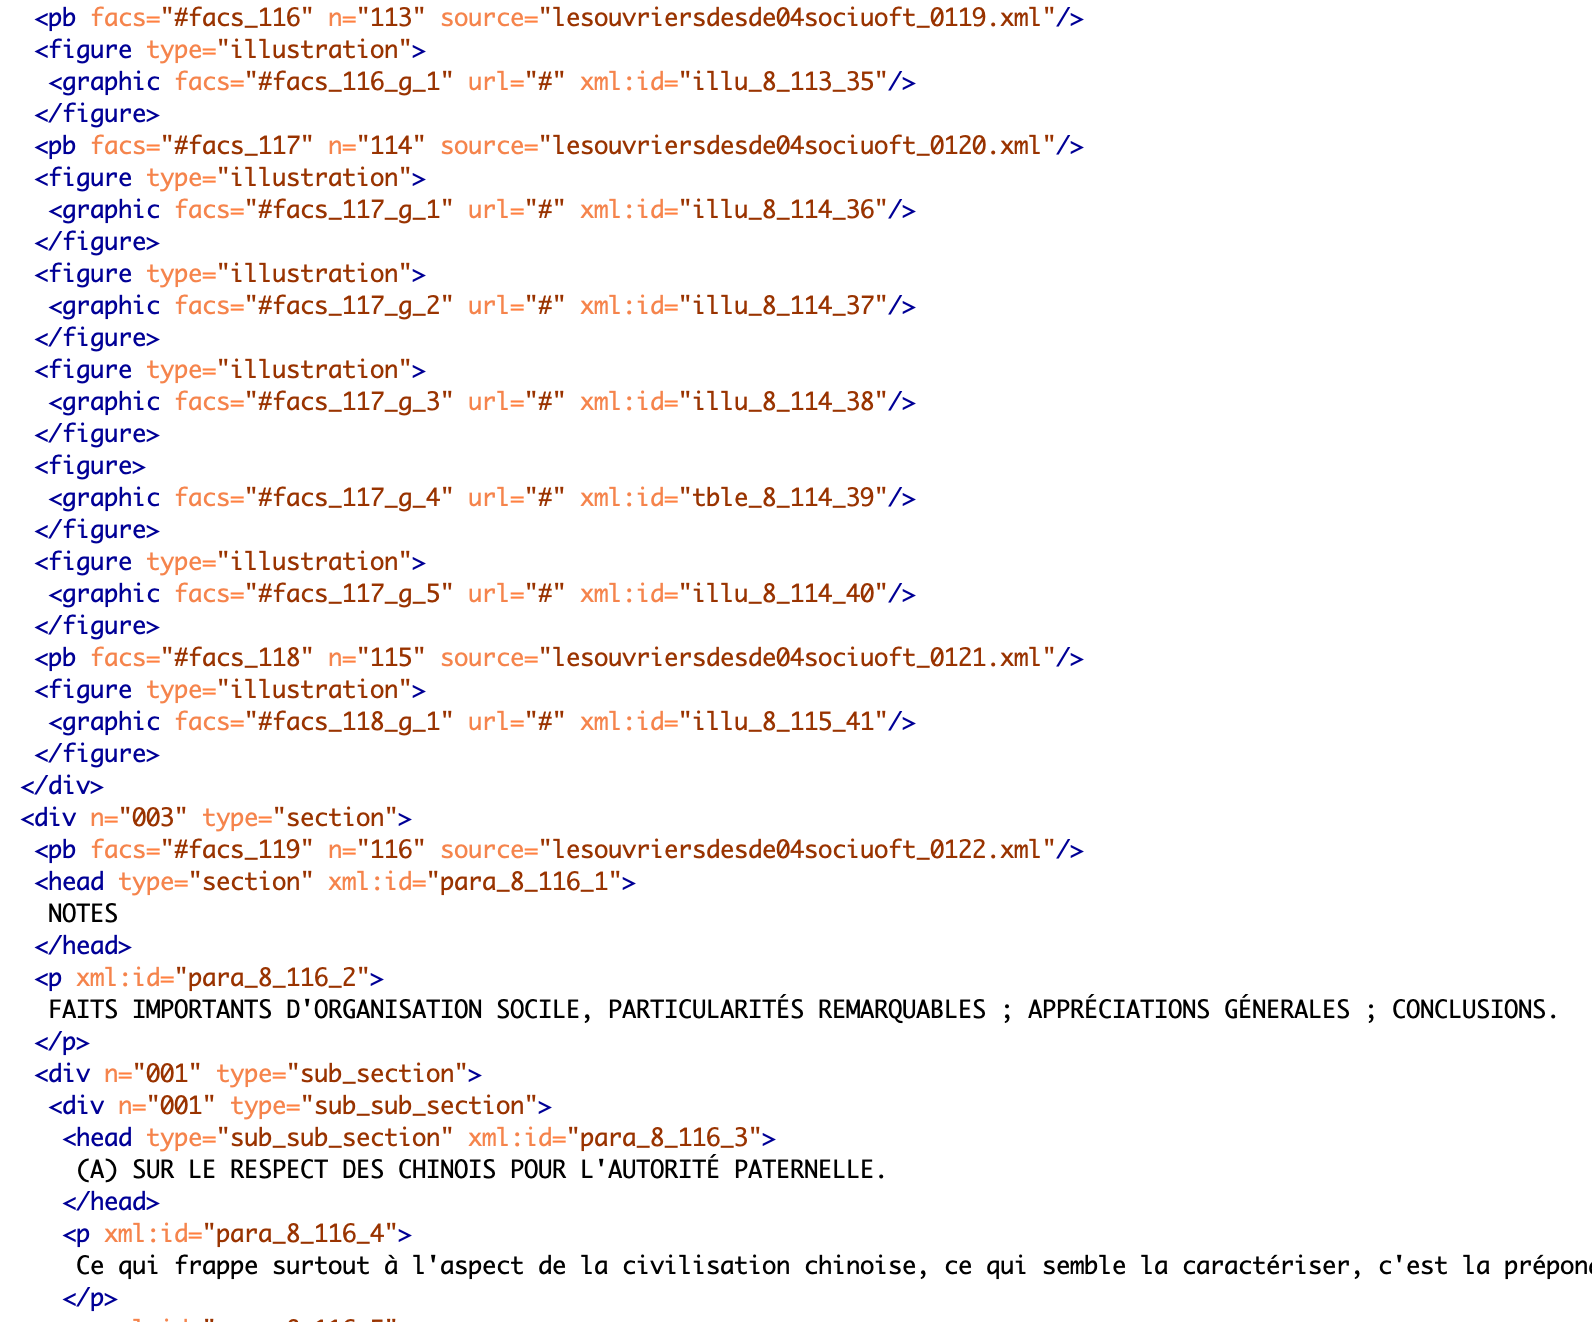
\includegraphics[width=15cm]{img/deficit_transcrip.png}
    \caption[Exemple d'un déficit de transcription]{Dans six fichiers, le contenu de la section \textit{Observations préliminaires} n'a pas été considéré comme du texte mais comme des figures. À l'inverse, la section \textit{Notes} a bien été prise en compte comme du texte. Exemple du fichier \texttt{s1t4\_chapt\_8.xml}.}
    \label{fig:deficit}
\end{figure}

Que s'est-il passé ? Le problème provient d'une fonction de \lse, \texttt{where\_do\_\-budgets\_start}. Son  rôle est de déterminer l'index de la page où commencent les tableaux de budget et de placer cette donnée dans la variable \texttt{budget\_start}. Pour cela, il cherche la ligne \og \textsc{budget des recettes de l'année} \fg, qui se trouve entre l'en-tête de la page et la ligne supérieure délimitant le tableau de budget. Une fois cette information connue, le script sait que la page correspondante et les suivantes jusqu'au commencement de la section \textit{Notes} (index placé dans la variable \texttt{budget\_stop}) devront être considérées comme des objets graphiques.

Or les trois monographies concernées dans le quatrième volume (\no{}~30, 33 et 37) présentent un problème au niveau de la segmentation de la première page du budget. En effet, soit l'en-tête a été considéré comme du texte et le reste comme une illustration (\fig{}~\ref{fig:odm30tkb} et~\ref{fig:odm33tkb}), soit l'ensemble de la page a été considéré comme une illustration (\fig{}~\ref{fig:odm37tkb}). \kraken, à qui les zones de segmentation sont adressées, n'a donc rien à transcrire (à l'exception de la ligne d'en-tête dans deux cas), et \lse{} n'obtient pas de résultat quand il cherche la ligne \og \textsc{budget des recettes de l'année} \fg{}. La variable \texttt{budget\_start} est équivalente à \texttt{false} et \lse{} considère que les budgets débutent à la première page de la monographie. Il remplace alors toutes les transcriptions par des objets graphiques jusqu'aux \textit{Notes} qu'il traite normalement, et nous obtenons un fichier partiellement transcrit.

\begin{figure}[t]
    \centering
    \begin{subfigure}{0.3\textwidth}
     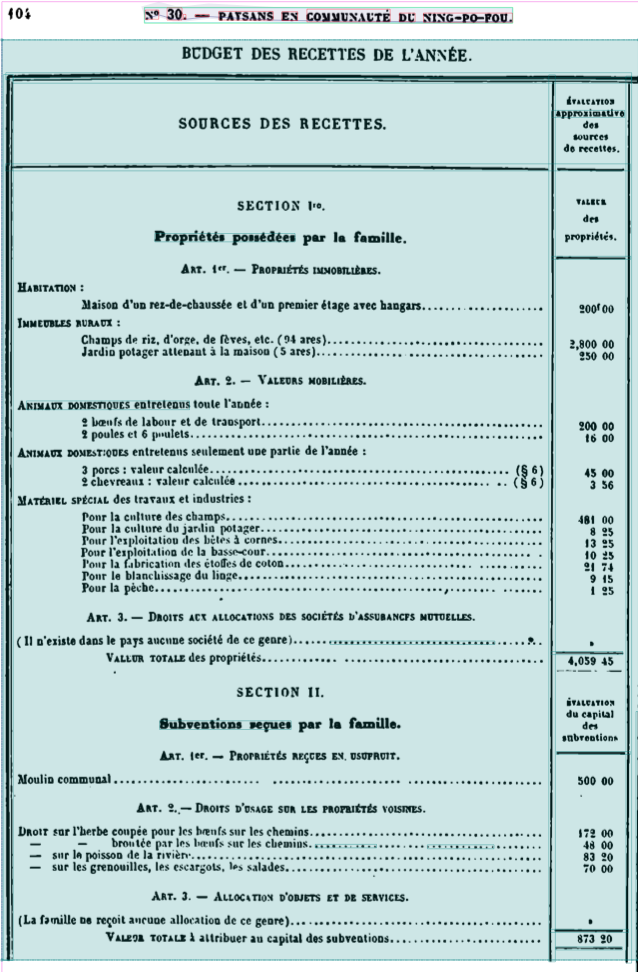
\includegraphics[width=1\linewidth]{img/transkribus_30.png}
     \caption{\no{} 30, p. 104.}
     \label{fig:odm30tkb}
    \end{subfigure}
    \hspace{5pt}
    \begin{subfigure}{0.3\textwidth}
     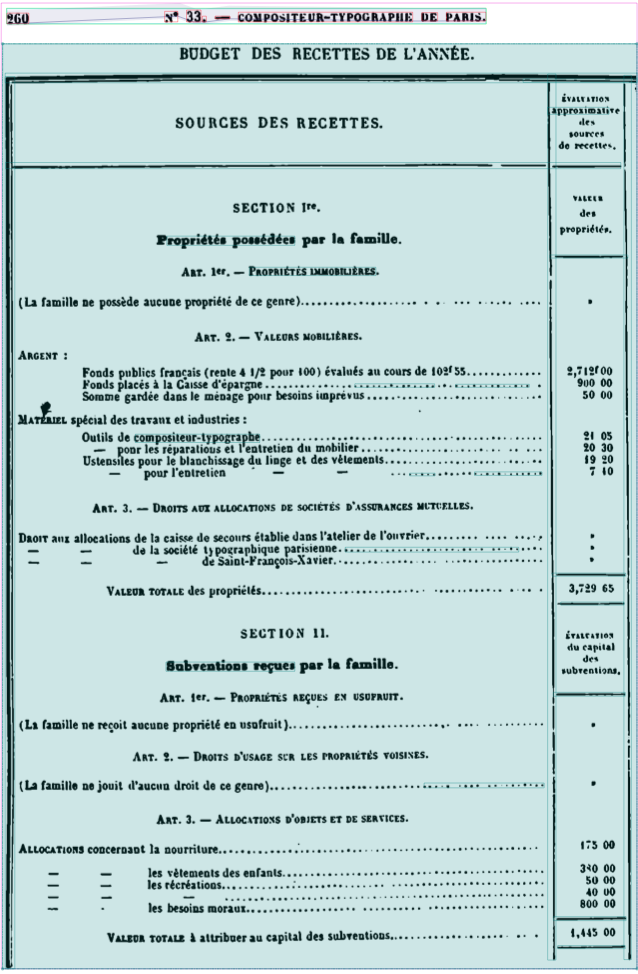
\includegraphics[width=1\linewidth]{img/transkribus_33.png}
     \caption{\no{} 33, p. 260.}
     \label{fig:odm33tkb}
    \end{subfigure}
    \hspace{5pt}
    \begin{subfigure}{0.3\textwidth}
     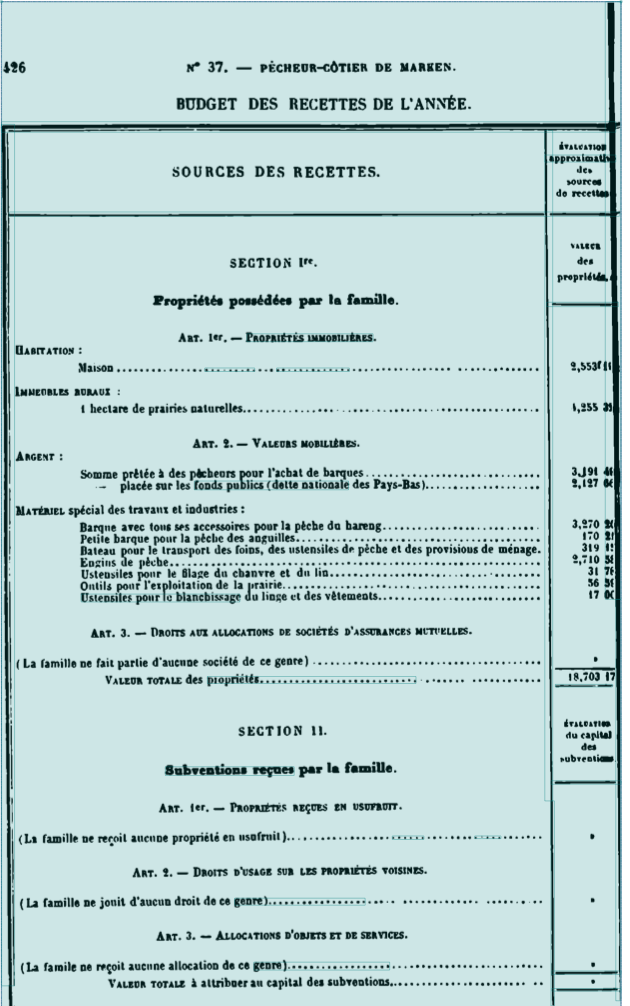
\includegraphics[width=1\linewidth]{img/transkribus_37.png}
     \caption{\no{} 37, p. 426.}
     \label{fig:odm37tkb}
    \end{subfigure}
    \caption[Segmentation défectueuse dans \transkribus{}]{Segmentations dans \transkribus{} des pages liminaires des budgets des monographies \no{} 30,  33 et 37. Dans les monographies 30 et 33, seul la ligne d'en-tête est considérée comme du texte.}
    \label{fig:odmtkbs1t4}
\end{figure}

Ces fichiers requièrent une nouvelle \ocr{} et une nouvelle structuration ; une correction par le biais d'une transcription manuelle ne fait en effet pas partie des possibilités acceptables pour l'équipe ALMAnaCH. Cette opération a été repoussée et nous n'avons pas eu à la mener. La reprise de ces six fichiers pourra cependant servir à valider les modifications apportées à \lse{} en tenant compte de l'ensemble des axes d'amélioration relevés au cours du stage et présentés dans ce mémoire. Notamment, l'éventualité de l'absence de valeur pour \texttt{budget\_start} pourrait 
être envisagée et traduite par un message d'erreur informant l'opérateur que le calibrage de la segmentation doit être changé.

\subsection{Identification, cartographie et inclusion}

Au-delà d'une vérification de la cohérence du découpage, cette étape de vérification avait pour but de reconnaître le contenu des fichiers, de leur associer un identifiant unique et de produire un fichier de cartographie ou \og \textit{mapping} \fg{} du corpus. Une partie des identifiants provenaient d'une bibliographie réalisée au format BibTeX\footnote{BibTeX est le logiciel de gestion de bibliographie du langage \LaTeX.} par Stéphane Baciocchi à partir de son exemplaire personnel du corpus.

Une partie seulement, car le fichier bibliographique ne s'intéressait qu'aux monographies, là où ALMAnaCH avait la volonté de travailler sur l'ensemble du corpus, monographies et fichiers de paratexte compris. Il a donc été nécessaire d'établir de nouveaux identifiants sur le modèle de ceux des monographies. Ces derniers se composent d'une série de trois chiffres suivie d'une lettre, \texttt{a} pour une monographie, \texttt{b} pour le précis \textit{bis} et \texttt{c} pour le \textit{ter} (\texttt{\textbackslash d\textbackslash d\textbackslash d[a-c]}). Pour poursuivre dans ce sens, nous avons choisi de donner au premier fichier de paratexte le numéro \texttt{401a} et de continuer jusqu'au dernier.

Trois versions de la cartographie ont été réalisées : la première contient uniquement les monographies, la seconde le paratexte et la troisième l'ensemble des fichiers\footnote{La troisième cartographie a été scindée en fonction des volumes afin de constituer l'annexe \ref{mapping} du présent mémoire.}. Ces versions sont enregistrées au format CSV : en texte brut, elles se présentent sous la forme d'une succession de lignes contenant des données (identifiant, intitulé puis libellé du fichier), ces données étant séparées par des virgules. Ces fichiers CSV peuvent ensuite être interprétés comme des tableaux, chaque ligne correspondant à une ligne tabulaire et chaque virgule à une séparation entre deux colonnes. Ce format, outre son extrême simplicité, a l'avantage d'être libre et de pouvoir être parsé par le langage Python\footnote{Parser un fichier consiste à le lire et à interpréter son contenu afin d’en extraire certains éléments.}. Les données peuvent donc être manipulées par un script.

Une fois les CSV constitués, il a fallu implanter les identifiants dans les fichiers TEI : il s'agissait de la première opération que nous avons pu automatiser. Après avoir relevé les identifiants et les libellés de fichier dans le CSV général pour constituer un dictionnaire Python (\texttt{dict\_xml = \{'401a': 's1t1\_chapt\_1.xml', etc\}}), le script ouvrait chaque fichier un par un. À l'aide de la librairie \texttt{BeautifulSoup}, il analysait ensuite l'arbre XML (\fig{} \ref{fig:xmltree1}, p. \pageref{fig:xmltree1}) et implantait l'identifiant comme valeur de l'attribut \texttt{@xml:id} de \texttt{<TEI>} et de l'attribut \texttt{@ana} de la première \texttt{<div>}.

La première exécution de ce script a permis de faire remonter une erreur dans la constitution des identifiants : la grammaire TEI n'autorise qu'un \texttt{@xml:id} unique commençant par une lettre dans chaque document, ce qui n'était pas le cas ici\footnote{\og \textit{Values for the \texttt{@xml:id} attributes must be unique within a single document, and \texttt{@xml:id} values must begin with a letter}\fg{} : \textit{TEI Guidelines, 3.10.2 Creating New Reference Systems} (\url{https://www.tei-c.org/release/doc/tei-p5-doc/fr/html/CO.html\#CORS2}, consulté le \today).}. Or il n'était pas possible de revenir sur ces identifiants, utilisés par d'autres chercheurs et chercheuses. La seule solution trouvée a été d'ajouter le préfixe \texttt{ID-} devant chaque identifiant afin de satisfaire aux règles de la TEI.

\begin{figure}
    \centering
    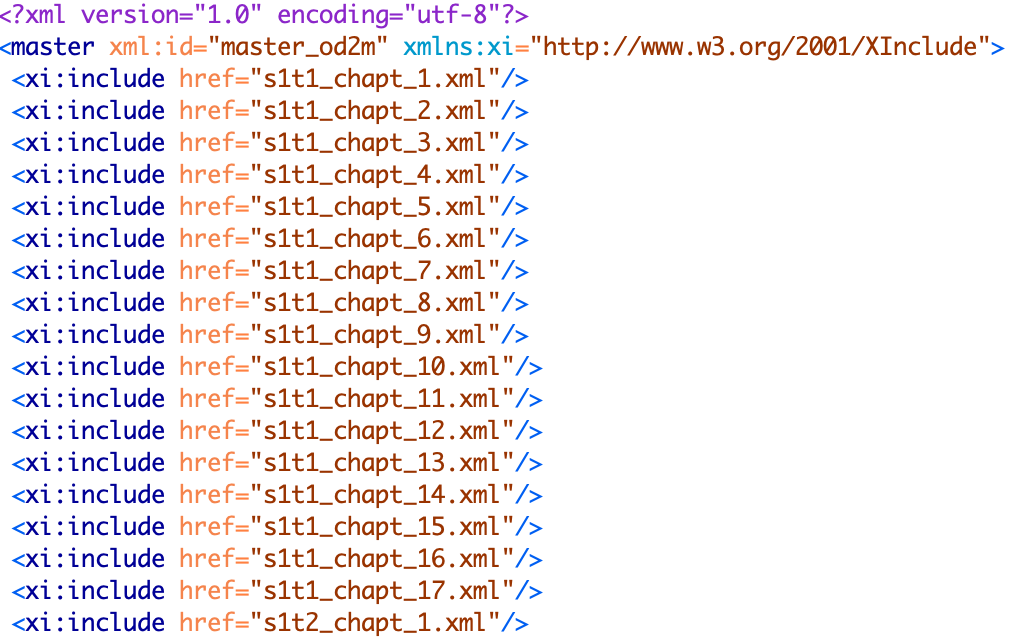
\includegraphics[width=15cm]{img/xinclude.png}
    \caption[Premières lignes du fichier \texttt{master.xml}]{Premières lignes du fichier \texttt{master.xml}. Dans la balise \texttt{<master>}, l'attribut \texttt{@xmlns:xi} contient l'adresse de l'espace de nom XInclude.}
    \label{fig:xinclude}
\end{figure}

ALMAnaCH souhaitait enfin pouvoir disposer d'un fichier XML regroupant l'ensemble des 194 fichiers. Pour cela, nous avons eu recours à un mécanisme d'inclusion grâce au langage XInclude.

Le principe est de constituer un fichier --- ici, \texttt{master.xml} --- dont le seul contenu est une balise \texttt{<master>} englobant une succession d'éléments \texttt{<xi:include>}. Ceux-ci possèdent un attribut \texttt{@href} contenant l'URI d'un fichier XML de paratexte ou de monographie. Il s'agit de l'identifiant uniforme d'une ressource (\textit{Uniform Resource Identifier}), \cad{} une séquence de caractères qui localise et nomme une ressource de manière pérenne\footnote{\og \textit{A URI is an identifier consisting of a sequence of characters matching the syntax rule named \texttt{<URI>}. It enables uniform identification of resources via a separately defined extensible set of naming schemes} \fg{} : RFC 3986, \textit{Uniform Resource Identifier (URI): Generic Syntax}, IETF, janvier 2005 (\url{https://tools.ietf.org/html/rfc3986}, consulté le \today).}. Dans notre corpus, les URI des fichiers ne sont pas leurs identifiants mais leurs libellés : au moment d'analyser \texttt{master.xml}, le logiciel --- par exemple, \oxygen{} --- va lui adjoindre le contenu de la ressource localisée par la première URI, \cad{} le fichier \texttt{s1t1\_chapt\_1.xml}, qui contient la page de titre du premier volume, puis passer à l'URI suivante (le premier paratexte du premier volume), et ainsi de suite jusqu'au dernier fichier du troisième volume de la troisième série.

Ce fichier \texttt{master.xml} a été là encore constitué de manière automatique avec un script qui rassemble tous les libellés des fichiers dans une liste et, pour chacun d'eux, écrit la ligne \texttt{<xi:include href="[libellé]"/>} (\fig{} \ref{fig:xinclude}).

\section{Vérification de l'encodage minimal}

La mise en forme minimale des documents a été correctement exécutée par \lse, aucune partie de la transcription n'ayant été laissée sans encodage.

\begin{figure}[h]
    \centering
    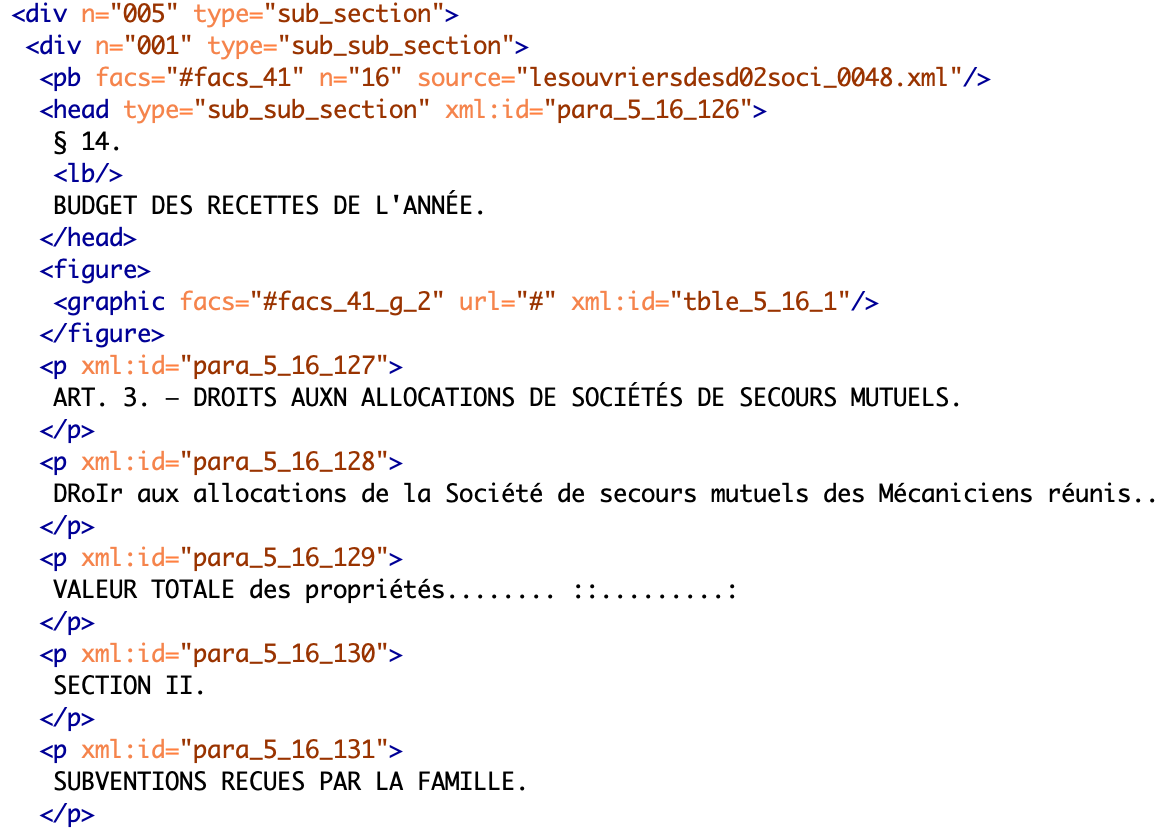
\includegraphics[width=15cm]{img/table_s2t2_chapt_5.png}
    \caption{Encodage du début du §14 de la monographie 56.}
    \label{fig:tableodm56xml}
\end{figure}

Les objets graphiques ont pu néanmoins poser problème au script. Nous avons vu dans la section précédente que dans six fichiers, toute une partie du texte avait été représentée par des éléments \texttt{<figure>}. L'inverse s'est également produit, \cad{} que des objets graphiques véritables --- à l'instar des tableaux de budget des paragraphes 14 à 16 --- ont souvent été considérés comme du texte. Ainsi, dans la monographie \no{} 56\footcite{mono056a}, le tiers du premier tableau du paragraphe 14 est encodé dans un élément \texttt{<figure>} (articles 1 à 2), le reste, à partir de l'article 3, étant transcrit et placé dans des \texttt{<p>} (\fig{} \ref{fig:tableodm56xml}).

Pour autant, ces faits sont moins gênants que les cas inverses, dans la mesure où il s'agit de surplus de transcription. Les \texttt{<div>} encadrant ces sections de budgets étant en place, il est envisageable d'effacer automatiquement les balises \texttt{<head>} et \texttt{<p>} qu'elles contiennent et de n'ajouter que des \texttt{<graphic>} avec l'adresse de l'image de la page.

Cependant, toute mesure d'ajout ou de suppression d'élément \texttt{<p>} ou \texttt{<head>} a pour conséquence de rompre la logique interne du document. En effet, ces balises possèdent un attribut \texttt{@facs} dont la valeur renvoie à l'identifiant (\texttt{@xml:id}) d'un élément \texttt{<zone>} dans les \texttt{<facsimile>}.

Pousser la précision de ces derniers jusqu'au niveau des paragraphes devient inutile puisque la correspondance entre les \texttt{<zone>} et les \texttt{<p>} ou les \texttt{<head>} ne peut plus 
être garantie. De fait, le niveau de référence devient la page (\texttt{<surface>}) et non le paragraphe. Les nombreuses modifications que nous avons menées sur ces balises nous ont donc conduit à retirer l'ensemble des éléments \texttt{<zone>} et des attributs \texttt{@facs} des paragraphes et des titres par le biais d'un script. Ce dernier a effectué un ensemble de 138263 suppressions de ligne dans le corpus. Dans l'arbre XML de départ (\fig{} \ref{fig:xmltree1} p. \pageref{fig:xmltree1}), le seul descendant de l'élément \texttt{<surface>} est désormais \texttt{<graphic>}.

\newpage
\thispagestyle{empty}
\mbox{}
\newpage

\chapter[Découpages éditorial et sémantique]{Contrôle des découpages éditorial et sémantique}

Le contrôle du découpage éditorial, \cad{} de l'implémentation de la structure logique, a donné lieu à la reprise la plus importante. Il s'agit d'un point crucial pour les fichiers des \odm, du fait de l'importance accordée par l'école leplaysienne à une structure logique qui seule permet de transformer les \og faits observés \fg{} sur le terrain en des \og faits décrits \fg{} par la monographie\footcite[p. 87]{baciocchi2}.

\section{Découpage éditorial}

\subsection{Niveau des titres (\texttt{<head>})}

Pour commencer, nous avons cherché à évaluer l'étendue des corrections à effectuer à l'aide d'un script. Il comparait une structure idéale --- \cad{} l'idée que chaque fichier de monographie devait contenir dans des \texttt{<head>} deux titres de niveau section (B et C), quatre titres de sous-section (I à IV) et seize titres de paragraphes (§1 à §16, \cf{} \ann{} \ref{structure}) --- à la structure réelle contenue les fichiers. Les titres qui n'avaient pas été trouvés étaient listés en sortie.

Le script a fait remonter plus de quatre cent cinquante erreurs. Ce chiffre comptait de nombreux faux positifs en raison de la non-prise en compte de la qualité des transcriptions. Certains titres étaient en effet présents mais leurs transcriptions étaient fautives. Les erreurs principales pouvaient néanmoins être identifiées dès cette étape :

\begin{itemize}
    \item Des distances d'édition trop faible entre deux titres avaient causé le remplacement de l'un par l'autre :
    \begin{itemize}
        \item (II.) \og Mode d'existence de la famille \fg{} par (III.) \og Moyens d'existence de la famille \fg.
        \item \og § 11. -- Récréations \fg{} par \og § 7. -- Subventions \fg.
    \end{itemize}
    \item La monographie \no{} 44\footcite{mono044a} est la dernière à posséder des titres de paragraphe sur une seule ligne, un retour à la ligne étant ensuite systématiquement effectué entre le numéro et le libellé du paragraphe. Cet élément n'avait pas été compris par \lse, qui a pu répéter ou non le numéro du paragraphe sur la ligne du libellé.
    \begin{itemize}
        \item En cas de répétition, le numéro original était placé dans un \texttt{<p>} et le titre avec le numéro ajouté dans un \texttt{<head>} (\fig{} \ref{fig:ex_structure} p. \pageref{fig:ex_structure}).
        \item En cas de non répétition, le titre n'était pas toujours détecté et les deux lignes étaient encodées dans des \texttt{<p>}.
    \end{itemize}
    \item Des titres transcrits avec une distance trop grande par rapport au modèle n'avaient pas été détectés. Ce point concerne l'ensemble des titres, sans prévalence particulière.
    \item Les titres des tableaux de budgets étaient souvent transcrits plus d'une fois.
    \item Les cas particuliers n'avaient pas été pris en compte :
    \begin{itemize}
        \item La monographie porte sur un ouvrier ou une ouvrière et non pas une famille, ce qui conduit à un changement dans la terminologie (par exemple, \og État civil de la famille \fg{} devient \og État civil de l'ouvrier \fg) : concerne notamment \texttt{s1t2\_chapt\_4.xml}, \texttt{s1t3\_chapt\_7.xml} et \texttt{10} ;
        \item Certains titres de paragraphe n'étaient pas séparés du texte mais imprimés en italique au début de celui-ci (\ann{} \ref{ann:structure-allegee}) ;
        \item Le titre n'est pas imprimé (\ann{} \ref{ann:titre-non-imprimes}, \ref{ann:structure-allegee} et \ref{ann:no-notes-no-16}) ;
        \item La monographie possède une structure qui lui est propre (\ann{} \ref{ann:remarques-et-cas-particuliers}).
        \item La sous-section des budgets est titrée dans huit monographies, mais ce titre n'a jamais été détecté comme tel par \lse.
    \end{itemize}
\end{itemize}

\subsection{Niveau des divisions (\texttt{<div>})}

L'implémentation de la structure logique ne s'est pas uniquement traduite par une mise en forme des titres : chaque \texttt{<head>} est en effet attaché à une \texttt{<div>} (\fig{} \ref{fig:deficit} p. \pageref{fig:deficit}). Tous deux possèdent un identifiant \texttt{@type} qui définit leur niveau (\texttt{section}, \texttt{sub\_section} ou \texttt{sub\_sub\_section}), la \texttt{<div>} étant en plus nantie d'un numéro (\texttt{@n}).

Trois erreurs ont été constatées à ce niveau :

\begin{itemize}
    \item Lorsqu'un titre n'était pas détecté, la \texttt{<div>} correspondante n'était pas créée et le paragraphe était intégré dans la division précédente, invalidant de fait l'ensemble de la numérotation ;
    \item Des \texttt{<div>} surnuméraires ont été implantées (\fig{} \ref{fig:ex_structure} p. \pageref{fig:ex_structure}) ;
    \item Au cour du stage, il a été décidé de placer le titre de la monographie dans une \texttt{<div>} de type \texttt{section}, ce qui impliquait une reprise dans l'ensemble des fichiers.
\end{itemize}

\subsection{\textit{Tabula rasa}}

Le nombre élevé de cas particuliers rendait impossible une automatisation complète de cette reprise. Nous allons d'abord exposer la méthode suivie pour le traitement des cas particuliers avant de rendre compte de celle utilisée pour le reste du corpus.

\subsubsection{Cas particuliers}

Les monographies d'ateliers (\texttt{s3t1\_chapt\_2.xml}\footcite{mono472a} et \texttt{s3t2\_chapt\_10.xml}\footcite{mono473a}) imposaient une reprise manuelle du fait de leur structure unique. De plus, dans ces fichiers, ainsi que dans certaines monographies de familles, plusieurs titres n'étaient pas détachés des paragraphes. Le recours à la balise \texttt{<head>} n'était pas possible pour les traiter, dans la mesure où elle constitue normalement un bloc séparé des \texttt{<p>}. Plusieurs solutions, toutes insatisfaisantes, ont été envisagées.

La plus légère consistait à signaler la mise en forme de ces titres (italique ou gras) par des balises de mise en valeur telles que \texttt{<emph style="italic">} ou \texttt{<hi rend="i">}. Nous n'avons pas opté pour ce choix en raison des règles de la TEI qui ne prévoient pas d'attributs pour caractériser ces balises (notamment, \texttt{@type}). Aussi n'aurait-il pas été possible de les différencier d'autres passages possédant une mise en forme similaire dans le corps du texte lors de la transformation des fichiers XML en d’autres formats.

Une deuxième solution, beaucoup plus lourde pour le fichier, aurait consisté en l'imbrication de  \texttt{<div>}. Le \texttt{@type} assigné à la division aurait permis de savoir que le \texttt{<head>} et le \texttt{<p>}, eux-même placés dans une sous-division, ne constituaient qu'un seul paragraphe dans le volume original (\fig{} \ref{fig:solution2}). La contre-partie est que chaque paragraphe aurait dû être placé dans une sous-division.

\begin{figure}[h]
    \centering
    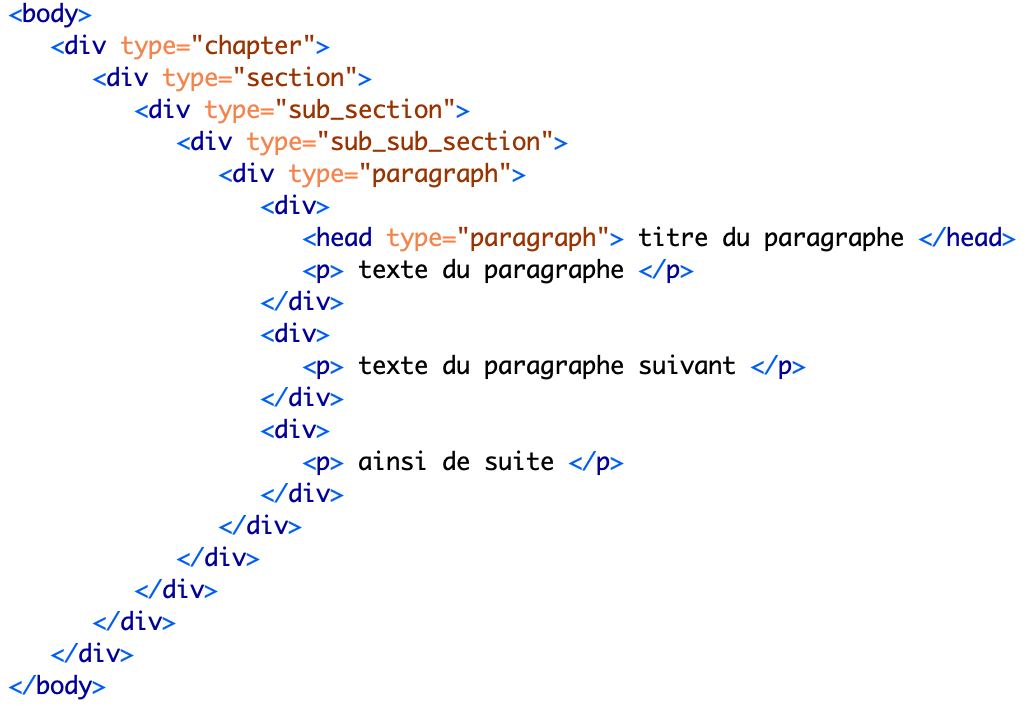
\includegraphics[width=15cm]{img/solution2.png}
    \caption[Proposition pour un encodage des paragraphes.]{Représentation de la deuxième solution, dont le résultat est de produire une imbrication malvenue de \texttt{<div>}.}
    \label{fig:solution2}
\end{figure}

Au final, \timeus{} n'a opté pour aucune solution, considérant que le nombre de cas était suffisamment bas pour ne pas avoir à mettre en place une solution particulière. Pour autant, cette décision n'a pas eu pour effet d'arrêter le niveau de granularité des titres à la sous-sous-section.

En effet, les fichiers \texttt{s1t5\_chapt\_9.xml}\footcite{mono041a} et \texttt{10}\footcite{mono042a} comprennent des précis de monographie dotés de leur propre structure logique et intégrés dans le corps de leurs sections \textit{Notes}. Les titres étant détachés des paragraphes, il a été possible de mobiliser un niveau inférieur à la sous-sous-section, le \texttt{paragraph}, afin de rendre compte de cette structuration.

\subsubsection{Reconstruction de la structure}

Ces cas particuliers réglés, il restait à prendre en charge l'essentiel du corpus, \cad{} une soixantaine de monographies. Une reprise entièrement manuelle n'était pas envisageable en raison du temps trop important qu'elle aurait nécessité. À l'inverse, une automatisation totale aurait nécessité une longue étude et un relevé minutieux des aléas de la détection et de la transcription des titres.

Nous avons donc choisi d'implanter la structure logique par des cascades d'expressions régulières appliquées sur un lot de fichiers à l'aide d'un script. Les expressions régulières sont des motifs qui permettent de décrire des chaînes de caractères dans un texte. Le module \texttt{re} de Python permet de mobiliser ces expressions dans un script, et notamment d'effectuer des substituions grâce à la fonction \texttt{re.sub()}.

Du fait de la désorganisation massive des \texttt{<div>}, la première expression régulière consistait à faire table rase de ces balises. Le script reconstruisait ensuite la structure en progressant selon ses niveaux. Il commençait par implanter la \texttt{<div>} de type \texttt{chapter} et celle de la première section (la page de titre). Venaient ensuite les \texttt{<div>} des deux sections restantes (\textit{Observations préliminaires} et \textit{Notes}), puis celles des sous-sections, etc.

Les expressions régulières recherchaient les libellés des titres lorsqu'il s'agissait de sections ou de sous-sections, car la plupart étaient convenablement transcrits. En revanche, il recherchait le numéro des sous-sous-sections, qui avaient tous pour point commun de commencer par le symbole typographique \texttt{§}. Les paragraphes \textit{Notes} des quatre-vingt-quatre premières monographies ayant pour particularité d'
être numérotés par une lettre entre parenthèses, le motif des sous-sous-sections des premiers lots était légèrement différent.

Une dernière commande, qui affichait la liste des balises \texttt{<head>} de chaque fichier, nous permettait de contrôler l'intégrité de la nouvelle structure. Si une erreur était constatée, nous intervenions manuellement afin de la résoudre. Pour chaque lot (qui correspondait \textit{grosso modo} à un volume), jusqu'à 50\% d'erreur était constaté. Cela était dû à des titres qui ne correspondaient pas aux motifs en raison de l'absence d'un symbole ou d'une transcription trop éloignée de la vérité terrain.

L'opération s'est conclue par la constitution automatique d'un tableau synoptique, le contenu de chaque balise \texttt{<head>} étant placé dans une cellule. Son étude a permis, d'une part, de corriger les dernières erreurs résiduelles, et d'autre part de rédiger une note exposant l'ensemble des défauts restant (\ann{} \ref{ann:releve_erreurs}).

\section{Découpage sémantique}

L'opération de reconstruction de la structure logique a mis en évidence une erreur qui n'avait pas été détectée jusque là : des en-têtes (rappel du type de chapitre et de son titre, numéro de page ou de la monographie) et des bas de page (numéro du cahier) étaient toujours présents dans le flux du texte. L'élément révélateur a été la mise en forme par \lse{} de plusieurs rappels de titre comme s'il s'agissait de titres à part entière. 

Pour les supprimer, nous avons là encore utilisé des expressions régulières. L'automatisation n'était pas possible pour les numéros de page, de cahier ou de monographie --- par exemple, \texttt{<p>3</p>} --- car certaines transcriptions de tableau avaient produit des données numériques semblables qu'il fallait conserver.

Pour résoudre ce problème, nous avons utilisé la fonction de recherche de l'outil \og projet \fg{} d'\oxygen, qui permet de rechercher une expression dans l'ensemble des fichiers du corpus. Les expressions étaient toutes construites par rapport à la balise \texttt{<pb/>} qui marque un changement de page, et toute occurrence d'une donnée numérique et d'un titre était systématiquement contrôlée (\fig{} \ref{fig:supprnumpage} et \ref{fig:suppnumcahier}).

Cette opération a permis de garantir que la reconstitution des paragraphes serait très peu perturbée par des éléments externes. Des contrôles visuels au cours d'autres actions ont cependant permis de déceler des numéros subsistants, placés à la fin de certains paragraphes ou bien transcrits par des lettres (\fig{} \ref{fig:suppnumcahiervisu}).

\begin{figure}
    \centering
    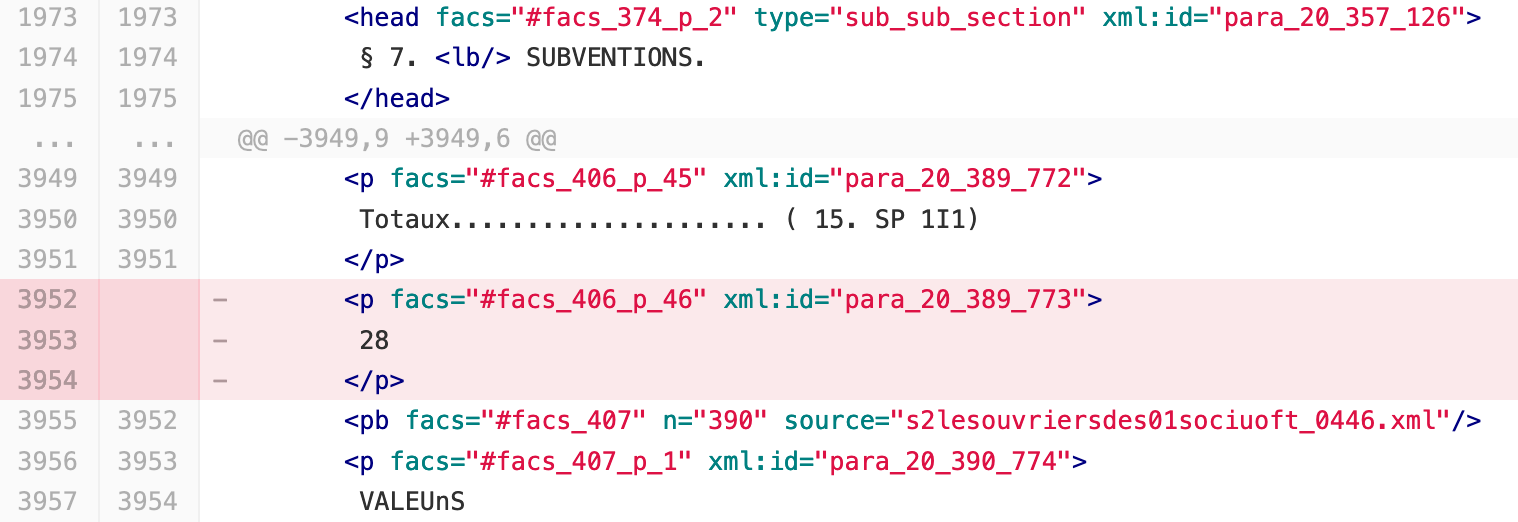
\includegraphics[width=15cm]{img/suppr_num_page.png}
    \caption[Suppression d'un numéro de page]{Suppression du numéro de page 28 dans le fichier  \texttt{s2t1\_chapt\_20.xml} (image du \commit{} sur \gitlab{} --- monographie \no{} 53).}
    \label{fig:supprnumpage}
\end{figure}

\begin{figure}
    \centering
    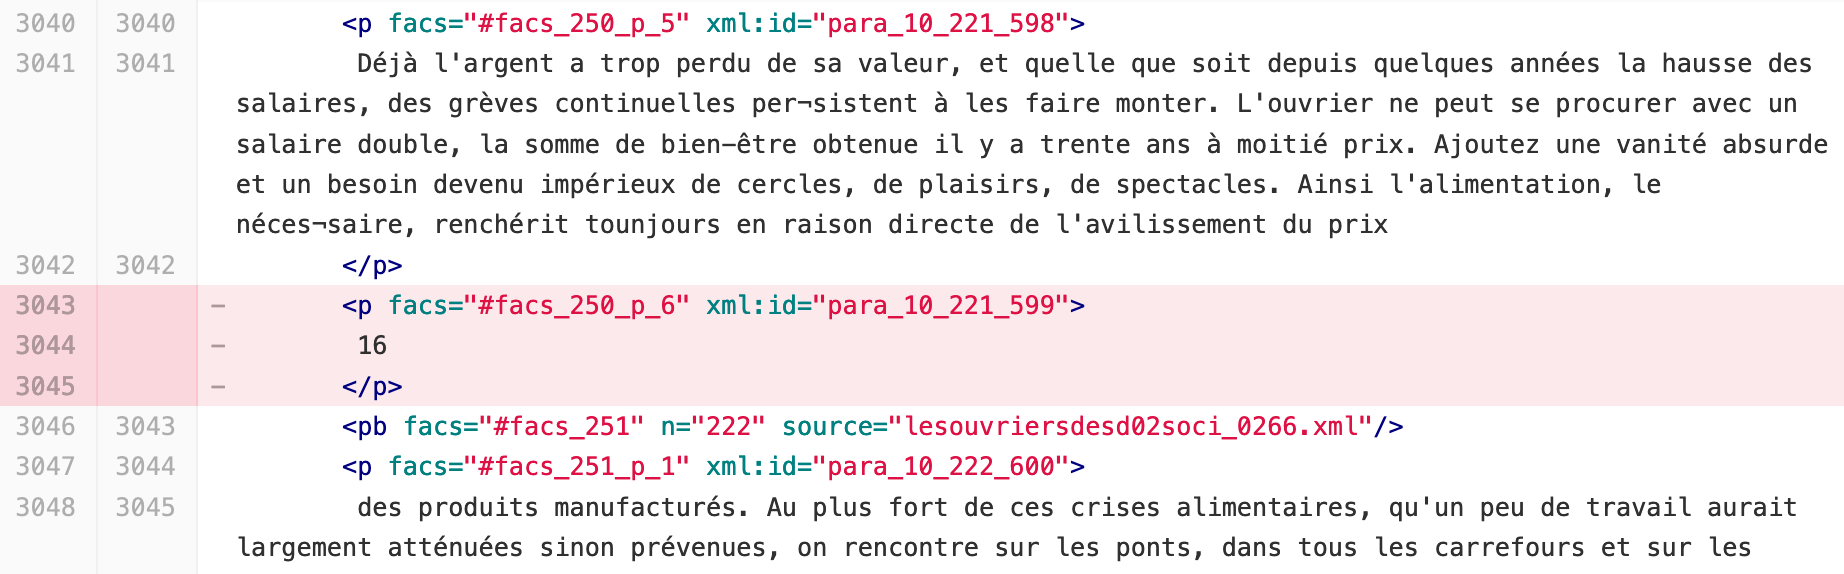
\includegraphics[width=16cm]{img/suppr_num _cahier.png}
    \caption[Suppression d'un numéro de cahier (1)]{Suppression du numéro de cahier 16 dans le fichier  \texttt{s2t2\_chapt\_10.xml} (image du \commit{} sur \gitlab{} --- monographie \no{} 59, page 221).}
    \label{fig:suppnumcahier}
\end{figure}

\begin{figure}
    \centering
    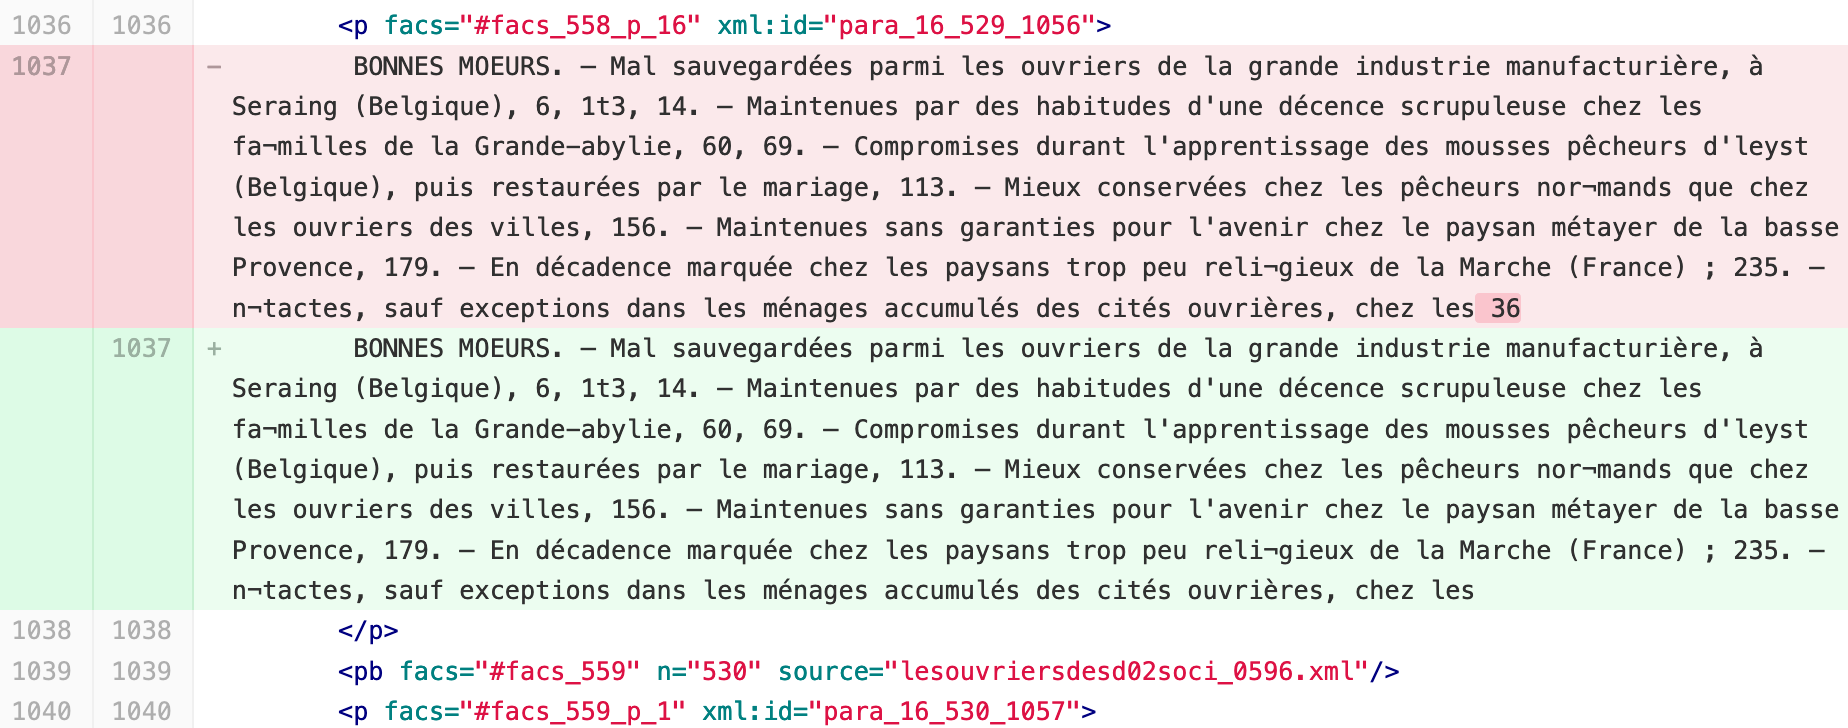
\includegraphics[width=16cm]{img/suppr_num _cahier_visuel.png}
    \caption[Suppression d'un numéro de cahier (2)]{Suppression du numéro de cahier 36 dans le fichier  \texttt{s2t2\_chapt\_10.xml} après un contrôle visuel (image du \commit{} sur \gitlab{} --- table alphabétique et analytique du deuxième volume de la deuxième série, page 529).}
    \label{fig:suppnumcahiervisu}
\end{figure}


\section{Validation du schéma XML-TEI}

Les erreurs de structuration et de transcription traitées dans les quatre premiers niveaux d'encodage, nous pouvions envisager de formaliser le schéma des fichiers. Il s'agit d'établir un document définissant quelles balises peuvent être utilisées dans les fichiers, réglant l'ordre de leur imbrication et arrêtant le nombre et la nature des attributs qui peuvent leur être attachés.

Nous avons choisi d'établir un fichier ODD, entièrement écrit dans une syntaxe XML, qui permet d'établir très précisément les éléments, les séquences d'éléments (nombre et ordre) et leurs attributs. \oxygen{} est capable d'en générer un après avoir analysé un ensemble de fichiers TEI, puis de le transformer en un schéma relaxNG. Ce document relaxNG contient le schéma servant à la validation du fichier TEI, l'ODD étant un fichier XML de documentation et de description de ce schéma. Le document relaxNG est finalement associé au document TEI (\fig{} \ref{fig:tei-odd-rng}), une des fonctionnalités d'\oxygen{} permettant de contrôler à tout moment la validité du code par rapport au schéma.

\begin{figure}[h]
    \centering
    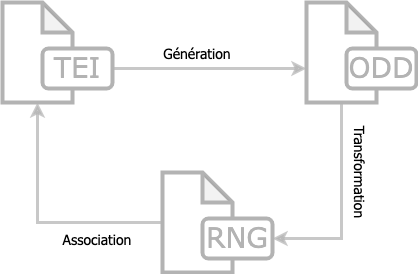
\includegraphics[width=5cm]{img/tei-odd-rng.png}
    \caption{Schématisation du processus de validation à l'aide d'une ODD.}
    \label{fig:tei-odd-rng}
\end{figure}

Le document ODD est généré automatiquement par \oxygen{} grâce au scénario de transformation du Consortium TEI intitulé \textit{oddbyexample}. Il s'agit d'une feuille de style XSL qui, appliquée à un document TEI, analyse l'ensemble des balises et leurs attributs pour les comparer aux préconisations de la TEI\footnote{\textit{The XSLT stylesheet which traverses a nominated directory tree looking for *.xml files which have <TEI> or <teiCorpus> root elements. It analyzes the collection of elements and attributes in the resulting corpus, and compares that to the whole of TEI P5} : \textit{oddbyexample} sur le \textit{TEI Wiki} (\url{https://wiki.tei-c.org/index.php/Oddbyexample}, consulté le \today).}. Puis il génère une ODD où les modules TEI sont chargés, les balises et les attributs non-utilisés étant supprimés d'office et les valeurs des attributs collectées et inscrites dans des listes.

\begin{figure}[h]
    \centering
    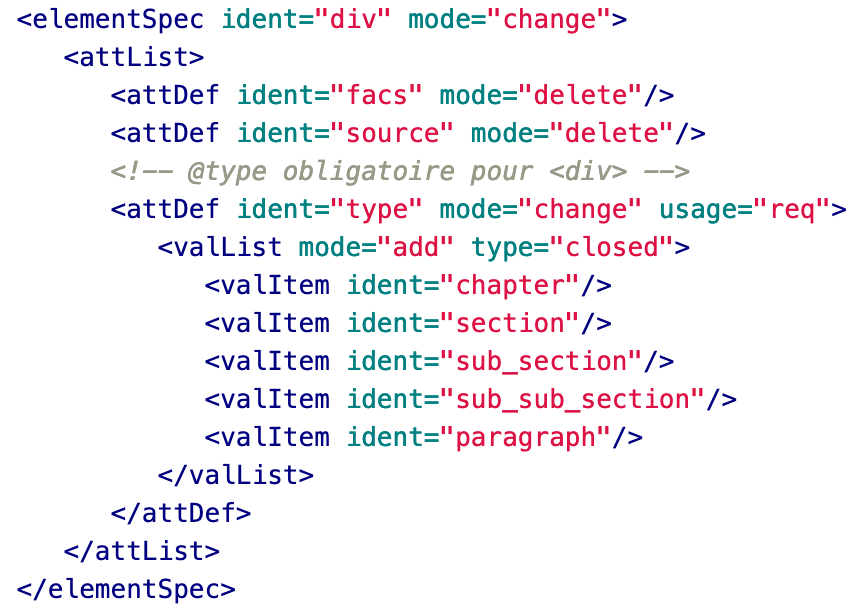
\includegraphics[width=9cm]{img/odd.png}
    \caption[Extrait de l'ODD concernant la balise \texttt{<div>}]{Extrait de l'ODD des \odm{} concernant la balise \texttt{<div>}. Les attributs \texttt{@facs} et \texttt{@source} sont supprimés (\texttt{mode="delete"}), \texttt{@type} est requis (\texttt{usage="req"}) et sa liste de valeurs est close (\texttt{type="closed"}).}
    \label{fig:tei-odd-rng}
\end{figure}

L'utilisateur peut modifier le document obtenu en imposant des règles plus restrictives ou au contraire en en relâchant certaines ; il peut également ajouter des valeurs d'attribut, rendre des attributs obligatoires ou contraindre l'enchaînement de certaines balises. Par exemple, nous avons rendu l'attribut \texttt{@type} obligatoire pour les balises \texttt{<head>} et \texttt{<div>}, et clos la liste de ses valeurs possibles (\fig{} \ref{fig:tei-odd-rng}).

Une ODD peut également être documentée, \cad{} que son rédacteur peut justifier ses choix d'encodage. Disposer d'un schéma et de sa documentation est un élément extrêmement important pour un projet en humanités numériques : c'est en effet une assurance pour la pérennité des données qu'il a rassemblées et structurées. Celles-ci ne sont plus dépendantes des ingénieur(e)s ou des structures institutionnelles et peuvent être réutilisées par d'autres projets\footcite[p. 61]{jolivet}.

Il existe plusieurs possibilités pour permettre la vérification du document TEI. La première et la plus courante est la spécification d'une instruction de traitement au début du document sous la forme suivante : \texttt{<?xml-model href="\#" type="application/xml" schematypens="http://relaxng.org/ns/structure/1.0"?>}, l'attribut \texttt{@href} devant être complété par l'adresse du schéma. Cela suppose bien évidemment que ce schéma soit hébergé, par exemple sur \gitlab. La ligne peut ensuite être ajoutée automatiquement à l'ensemble des fichiers du corpus grâce à la fonction de recherche et de remplacement.

Une autre possibilité est une validation externe, \cad{} qu'un logiciel ou un script vérifie la compatibilité des fichiers par rapport à un schéma qui lui est fourni par l'utilisateur à l'instant \texttt{t} de la validation. C'est une des fonctionnalités du mode \og projet \fg{} d'\oxygen. \timeus{} a cependant souhaité se détacher de tout logiciel, et \textit{a fortiori} d'un logiciel propriétaire, afin de se réserver la possibilité de contrôler la validité de ses fichiers à tout moment.

Le module \texttt{etree} de la librairie Python \texttt{lxml}, qui permet d'analyser un arbre XML, possède un outil répondant parfaitement à ce besoin. En effet, un schéma RNG peut être chargé avec la méthode \texttt{.RelaxNG()}, \texttt{validate()} contrôlant ensuite la validité de tout fichier lui étant donné comme argument par rapport à ce schéma.

La spécificité de ce script est qu'il s'applique à un corpus entier, ce qui avait pour effet d'allonger démesurément son exécution sur notre ordinateur (environ une demi-heure pour traiter une vingtaine de fichiers). Nous avons donc charger l'ensemble des fichiers, le schéma et le script sur le \textit{cluster} \rioc{} d'Inria, ce qui a considérablement rétréci le temps d'exécution  (vingt-quatre minutes au total).

\clearpage

\vspace*{\stretch{0.3}}

La structuration automatique des fichiers des \odm{} par le script \lse{} a donc été contrôlée selon différents niveaux d'encodage.

Sur le plan méthodologique, ce contrôle s'est traduit par plus d'interventions automatiques que manuelles, illustrant le gain de temps que la technologie peut apporter dans la production d'un corpus numérique. Sur le plan scientifique, ces problèmes montrent l'importance de la modélisation d'un corpus physique avant toute entreprise de rédaction d'un script de traitement. Nombre d'erreurs ont en effet été causées par une souplesse très faible d'\lse{} face aux cas particuliers du corpus. Cet effort de modélisation ne peut être mené que si un temps lui est alloué dans le projet.

La modélisation permet également de s'assurer de la pérennité des données. En effet, les fichiers des \odm{} n'existent pas dans le seul objectif de produire une édition numérique, \cad{} d'être mis en scène à travers une interface de consultation. Le processus de valorisation des données de la recherche peut emprunter deux voies différentes. L'une consiste à inscrire ces données dans le temps long et à favoriser leur ré-utilisation grâce à une structuration standardisée et documentée. L'autre entraîne leur publication dans un cadre institutionnel et budgétaire conjoncturel qui, s'il peut produire des résultats visibles rapidement, n'est pas assuré d'être reconduit et pérennisé.

Les fichiers des \odm{} se trouvent face à cette injonction qui, sans être réellement paradoxale, conjugue une obligation --- publier avant la fin du programme ANR \timeus{} --- et une ambition --- assurer la pérennité d'un corpus numérique.

Plusieurs voies sont envisagées pour répondre à ces nécessités. Aucune n'a pu être mise en place au cours de notre stage, mais nous avons mené plusieurs réflexions et quelques actions en leur sens. Nous allons d'abord présenter celles qui concernent les objets graphiques, puis nous intéresser à l'état des transcriptions, avant de conclure sur les différents types d'édition possibles et ce qu'ils impliquent pour les données issues du traitement automatique des fichiers des \odm.

\vspace*{\stretch{1.7}}

\newpage
\thispagestyle{empty}
\mbox{}
\newpage
\cleardoublepage
\part{Des données à valoriser}

\clearpage
\thispagestyle{empty}
\cleardoublepage

\chapter{Données graphiques, données chiffrées}

\section{Le lien entre le texte et les images du texte}

Dans chaque élément \texttt{<facsimile>}, une balise \texttt{<surface>} définit le bloc de segmentation supérieur (la page). L'élément suivant, \texttt{<graphic>}, indique dans son attribut \texttt{@url} la localisation de l'image de la page segmentée. L'ensemble des images étant stocké dans l'espace alloué au programme \timeus{} au sein du service \sharedocs{} de la TGIR Huma-Num, la localisation consiste en un chemin relatif (\fig{} \ref{fig:facsimile} p. \pageref{fig:facsimile}).

Or ces images sont déjà hébergées par \ia. Elles ont été téléchargées sur le \sharedocs{} dans le but de permettre leur segmentation par \textit{FineReader} et \transkribus{} puis leur \ocr{} par \lse. Leur conservation après l'obtention des fichiers XML n'est plus aussi pertinent que celle des prises de vues des registres prud'homaux effectuées dans des dépôts d'archives, qui n'existent sous aucune autre forme. Rappelons également qu'\ia{} se donne pour objectif d’être un centre stable et durable d’archives digitales ; aussi est-il peu probable que les images des \odm{} disparaissent de ses serveurs. Il nous a donc été demandé de substituer le chemin local par l'adresse de l'image sur \ia{} (\ann{} \ref{ann:feuille_route}, \issue{} 2) ; cette mission a donné lieu à la publication d'un billet sur le carnet de recherche du programme \timeus\footcite{genero}.

Nous avons apporté deux solutions : l'une employait les URLs basiques des images, l'autre mobilisait les manifestes \iiif{} des volumes. Toutes deux ont donné lieu à des scripts Python dont les fonctionnements sont similaires.

Les URLs se trouvaient dans des fichiers JSON renseignés dans le code source des pages d'\ia. Un fichier JSON contient des informations représentées de manière structurée ; il s'agissait ici de métadonnées concernant le volume numérisé. Parmi celles-ci, une sous-section intitulée \texttt{data} contenait des métadonnées (longueur, largeur, etc.) et l'URI de chaque image. Ces images étaient au format JPEG et correspondaient à celles déposées sur le \sharedocs. 

Le problème posé par cette solution est que les adresses n'étaient pas stables. En effet, au bout d'un certain temps, elles ne fonctionnaient plus car les informations avaient changé dans le fichier JSON source.

Aussi avons-nous exploré la piste du \iiif. L'\textit{International Image Interoperability Framework} permet d'afficher une image avec ses métadonnées dans le contexte d'une application web directement depuis le serveur où elle est stockée (ici, \ia). Les URLs de cette deuxième solution se trouvent dans les \og manifestes \iiif{} \fg{} des volumes : il s'agit des documents JSON contenant leurs métadonnées et référençant les points d'accès aux images (\cad{} leurs URIs dans le protocole \iiif).

Si ces images possèdent le même format que celles de la première solution, leur qualité est bien supérieure et permet d'effectuer des agrandissements d'une très grande profondeur. Du reste, le \iiif{} permet également de naviguer dans un volume en passant de page en page. Cette seconde solution est ainsi plus intéressante pour le projet \timeus{} dans la mesure où elle lui permet d'accéder d'une manière relativement simple à un document contenant un ensemble de données et de métadonnées qui pourront être valorisées au moment d'une édition en ligne.

Le script dont il est ici question, s'il se limite à insérer les URIs des images dans le code XML, commence par effectuer une requête pour lire le contenu des manifestes \iiif{} des \odm{}. Pour cela, il lit un CSV où nous avons enregistré les identifiants donnés par \ia{} aux numérisations, et les utilise pour compléter l'adresse des manifestes (\texttt{https://iiif.archivelab.org/iiif/<itemid>/manifest.json}). Ces lignes de code peuvent être réutilisées, probablement sous la forme d'une fonction, pour obtenir tout type de métadonnées issues des manifestes. En plus de rationaliser le stockage sur le \sharedocs{}, ce script prépare donc l'étape de la publication en ligne.

\section{Les données graphiques dans le flux textuel}

Un des principaux apport du \iiif{} pourrait être le traitement des objets graphiques qui, nous l'avons vu, sont nombreux dans les pages des \odm{} (\fig{}~\ref{fig:ex_figures} p. \pageref{fig:ex_figures}). En particulier, les photographies, les figures ou les cartes pourraient bénéficier des fonctionnalités d'agrandissement afin de permettre à l'utilisateur de pleinement les prendre en considération.

Pour rendre cela possible, il faudrait disposer d'une évaluation du taux de détection des figures. Ce chiffre n'est pas connu, mais des relevés aléatoires laissent penser qu'il risque d'être inférieur à 60\%. Les tableaux sont les figures qui ont posé le plus de problème au script, nous y reviendrons.

Parmi les autres, plusieurs n'ont été que partiellement détectées. La carte de la page 439 de la monographie \no{} 90\footcite{mono090a} est ainsi parfaitement détectée et transposée dans un élément \texttt{<figure>} (\fig{} \ref{fig:odmfig90439}). À l'inverse, le plan d'une \og habitation cambodgienne à Pnom-Penh \fg{} est détecté en double --- peut-être en raison de la superposition d'une vue de face de l'habitation et de son plan --- et le titre de la figure est transcrit comme du texte (\fig{} \ref{fig:odmfig90453}). Dans la monographie suivante\footcite{mono090b}, la photographie pleine page \og Cambodgiens et amanites \fg{}, insérée entre les pages 484 et 485, a été retirée du texte et n'est pas présente dans les fichiers sous quelque forme que ce soit.

\begin{figure}
    \centering
    \begin{subfigure}{0.4\textwidth}
     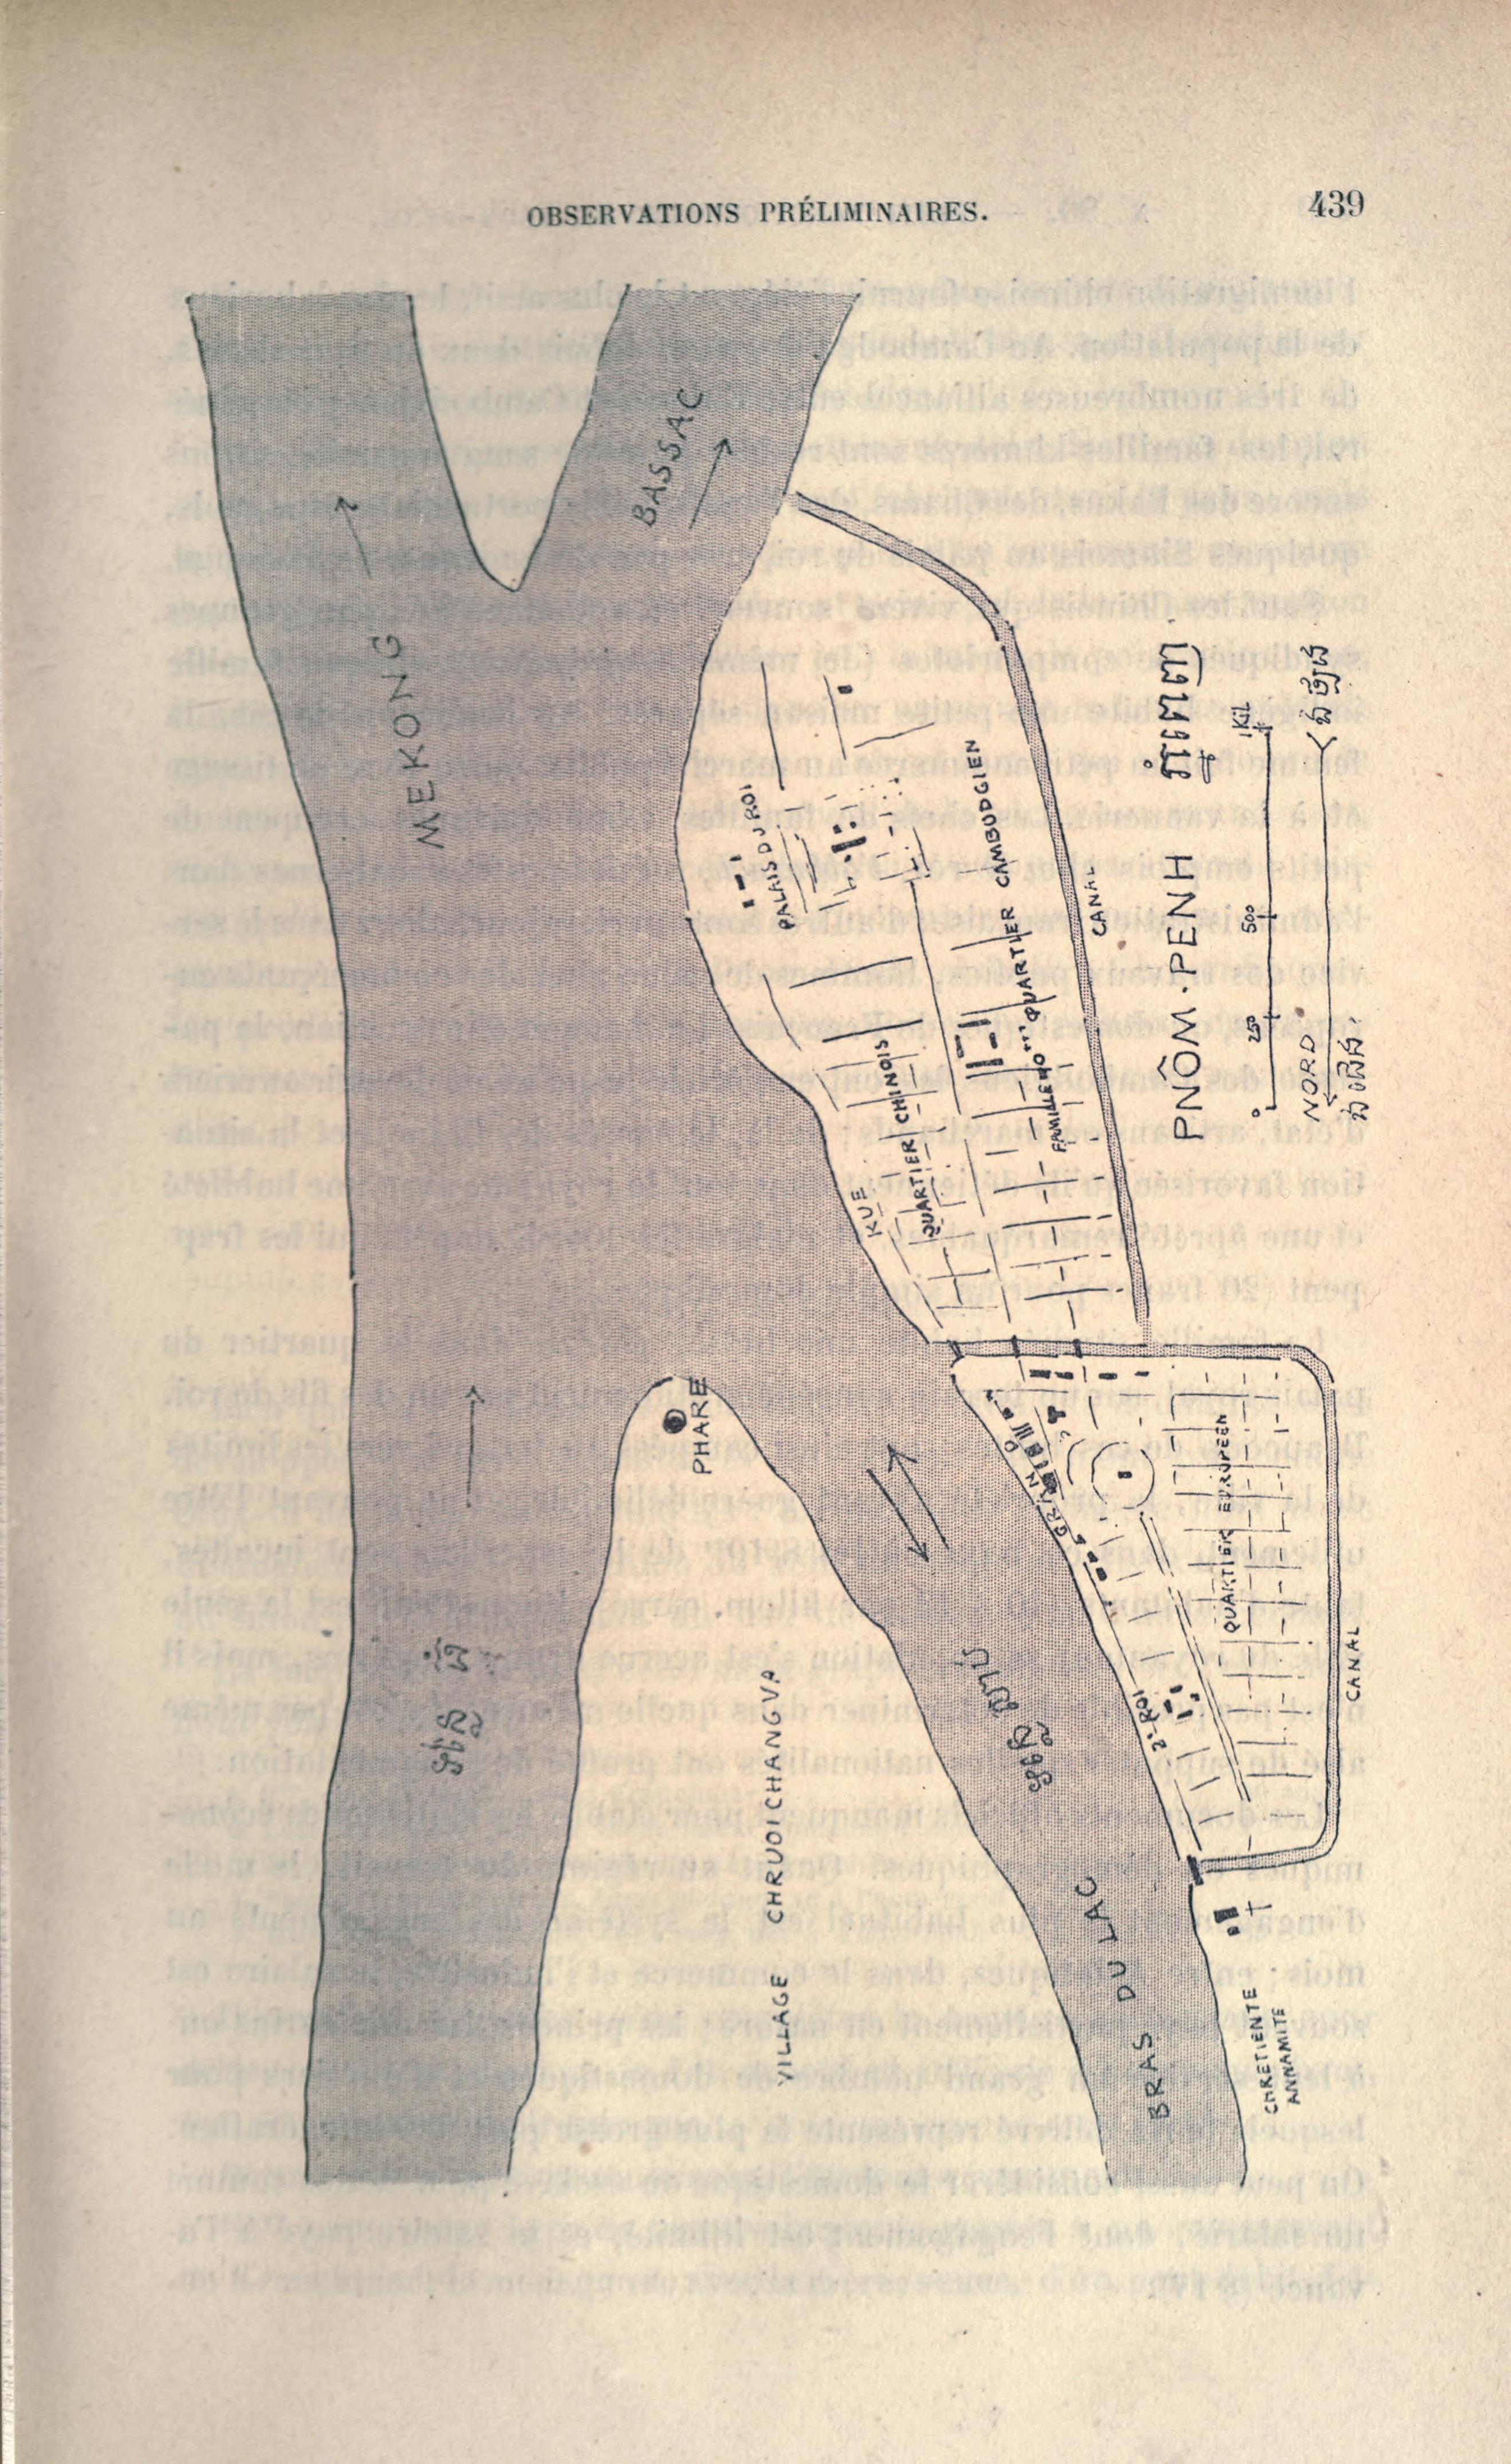
\includegraphics[width=1\linewidth]{img/odm90_439.jpg}
     \caption{Page 439 : détection optimale de la carte.}
     \label{fig:odmfig90439}
    \end{subfigure}
    \hspace{5pt}
    \begin{subfigure}{0.4\textwidth}
     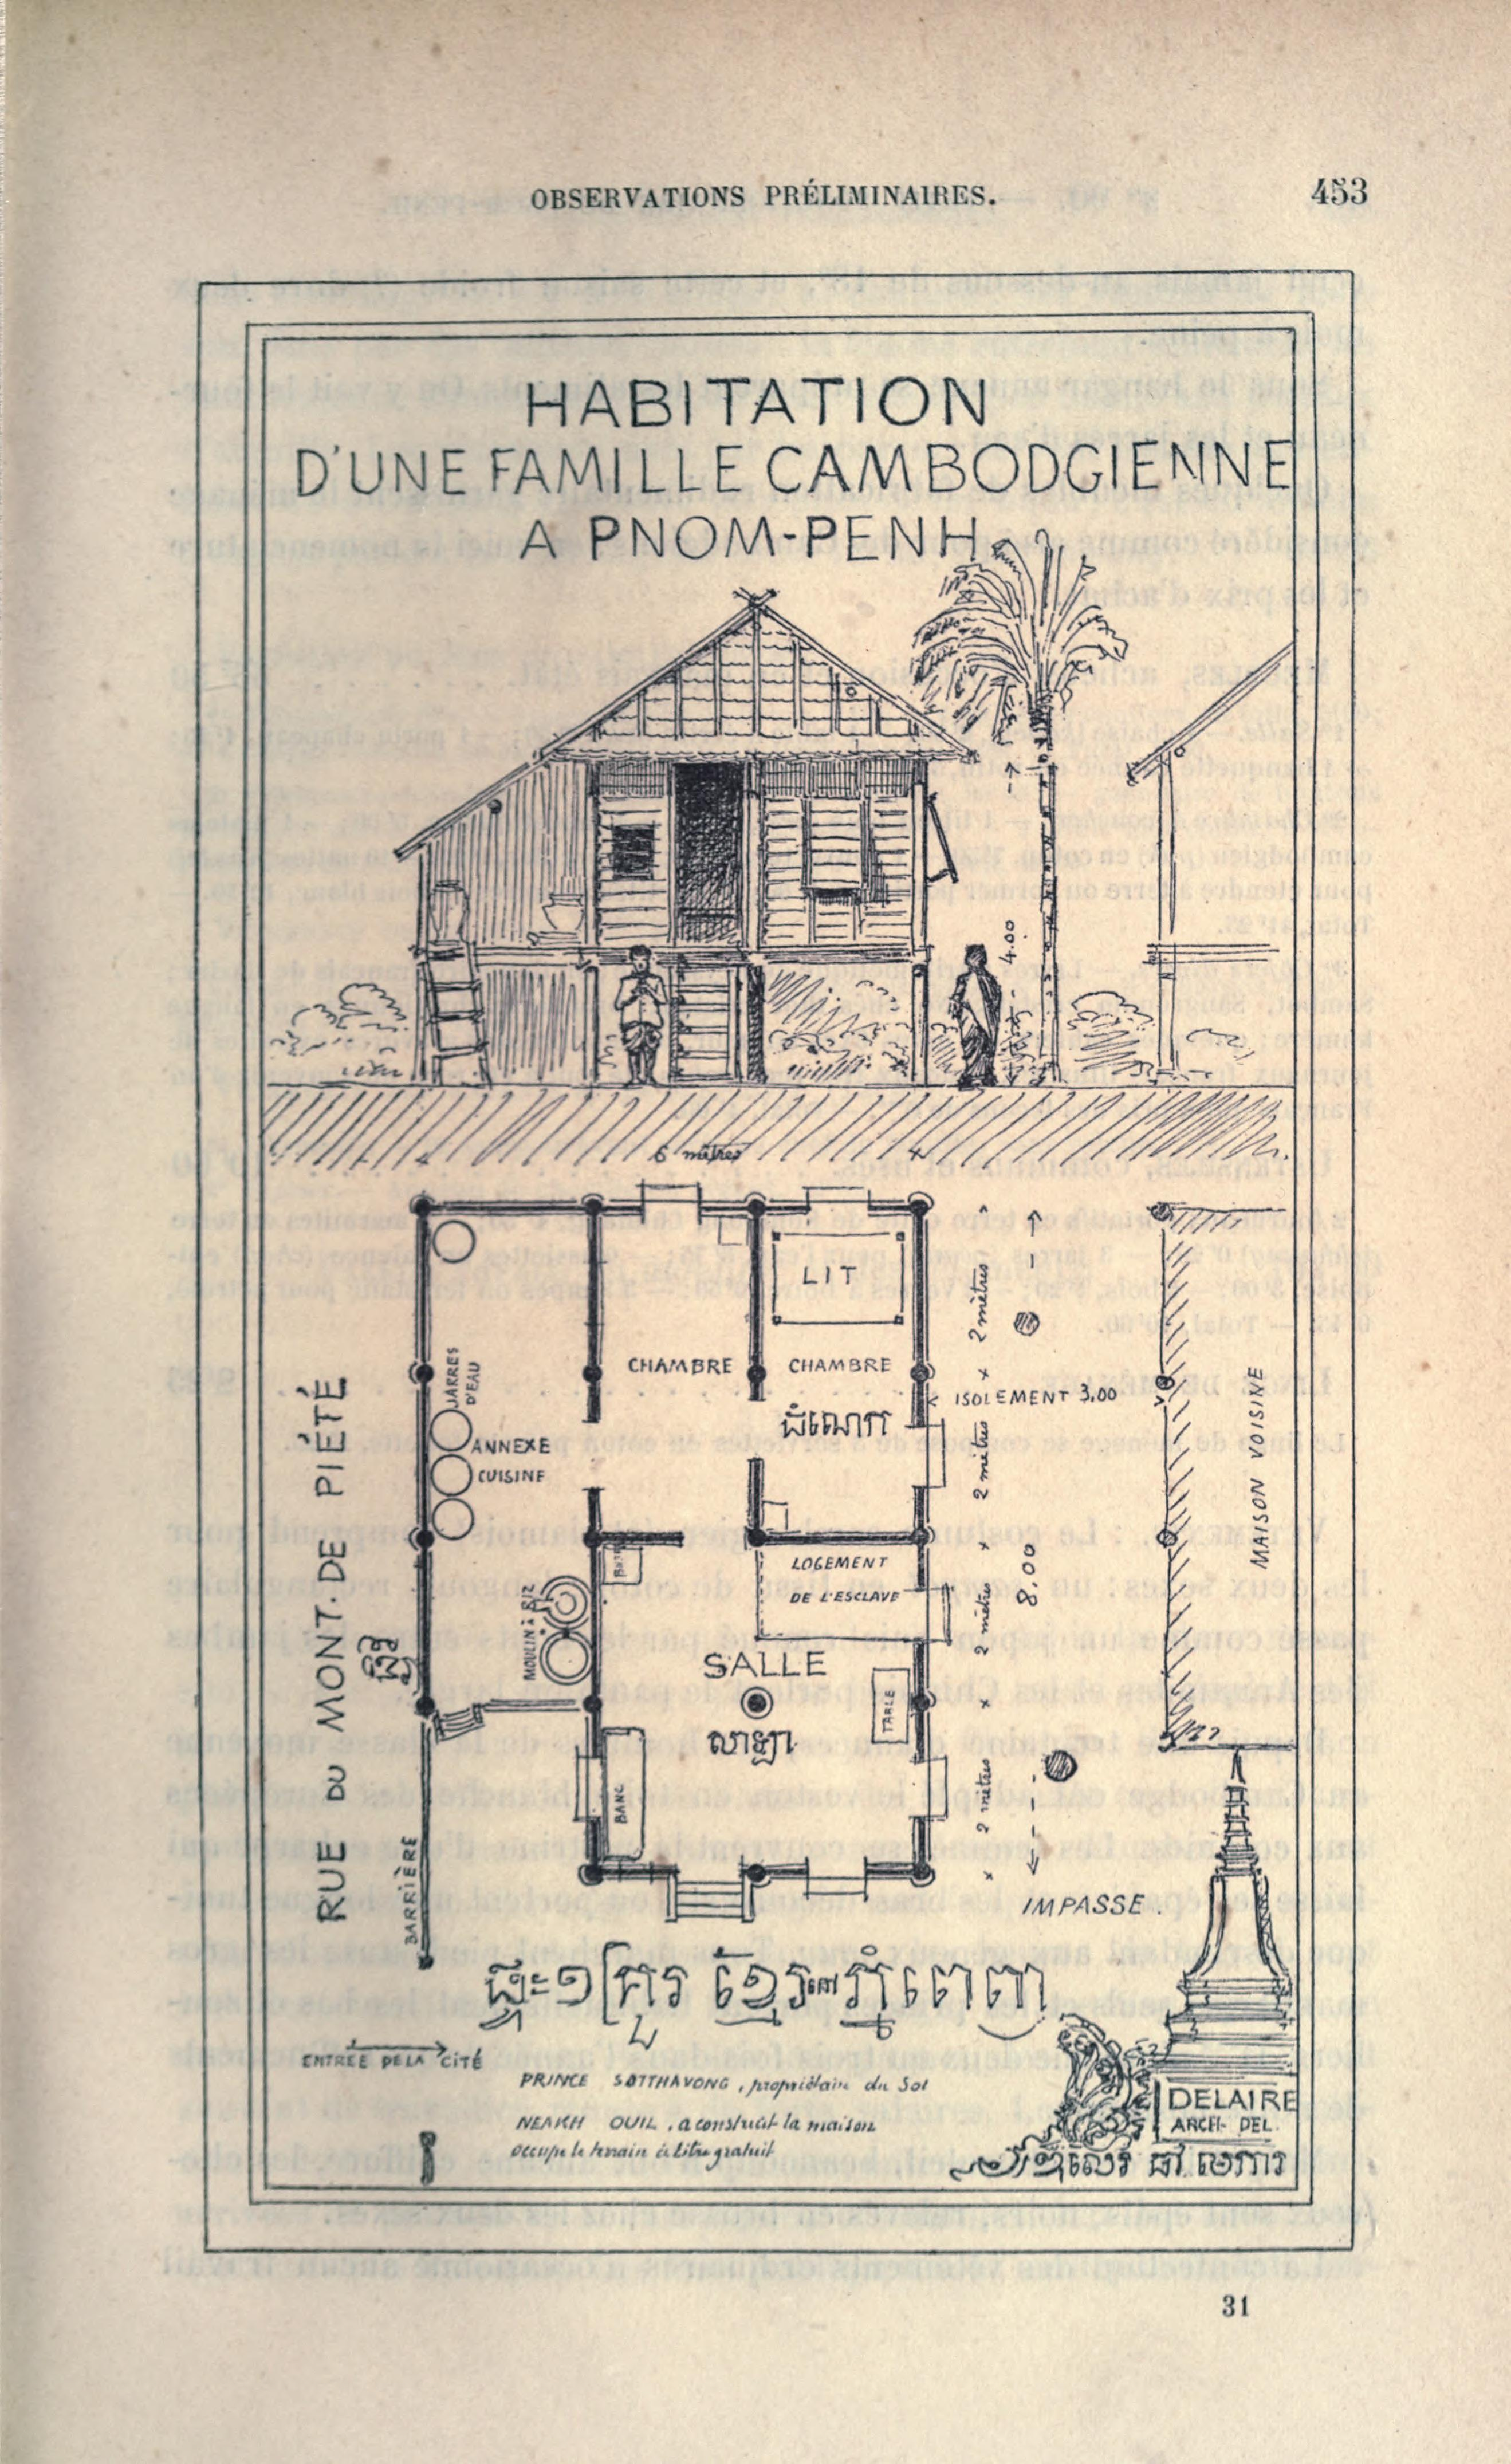
\includegraphics[width=1\linewidth]{img/odm90_453.jpg}
     \caption{Page 453 : détection en double et transcription du titre.}
     \label{fig:odmfig90453}
    \end{subfigure}
    \caption{Figures dans la monographie \no{} 90.}
    \label{fig:odmfig90}
\end{figure}

Ces erreurs de détection ne peuvent pas être résolues de manière automatique : aucune table des figures n'est présente dans les volumes. Un tel outil eut permis de cibler les pages à contrôler et de ne pas avoir à chercher visuellement les figures. Une intervention manuelle, possiblement longue, s'impose donc.

La présence de ces figures est également un élément à garder à l'esprit au moment de la reconstitution des paragraphes. En effet, certaines sont insérées en plein milieu de ces derniers. Pour ne pas perturber la reconstitution, il sera nécessaire d'ajouter une condition spécifiant que les balises \texttt{<p>} commençant pas une minuscule ne constituent pas une unité indépendante, et ce même si elles sont précédées d'une figure. Le problème de cette méthode est qu'elle présuppose que \lse{} a bien fait la différence entre une majuscule et une minuscule en début de phrase, ce dont on ne peut pas être totalement certain.

Ajoutons enfin que les figures de type carte, croquis ou photographie ont une importance relative du \pov{} de la donnée pure. Elles ne sont pas utiles aux chercheurs et aux chercheuses qui s'intéressent au vocabulaire du textile ou du monde ouvrier, ni à ceux qui souhaitent recueillir des données chiffrées. Dans le document XML, elles ne sont que des repères dont la nécessité ne se révélera qu'au moment de la transformation des fichiers pour une interface de visualisation.

\section{Les tableaux : images ou données ?}

À l'inverse, les tableaux qui jalonnent le corpus ont une importance considérable en raison des informations statistiques qu'ils contiennent. Plus particulièrement, les budgets des paragraphes 14 à 16 constituent \og la pièce centrale \fg{} des monographies leplaysiennes\footcite[p. 317]{savoyecontinuateurs}. Les \textit{Observations préliminaires} sont en effet entièrement tournées vers leur établissement ; le monographe n'arrête son enquête que lorsqu'il a établi un budget équilibré offrant une vue globale des recettes et des dépenses de la famille. En effet, dans la démarche de Frédéric Le Play, \og l'argent est pris comme unité de mesure de la vie sociale, le budget étant la quantification, en termes de revenus et dépenses, de l'ensemble des activités de la famille \fg\footcite[p. 317]{savoyecontinuateurs}.

D'un \pov{} technologique, il n'est cependant pas simple de reproduire à l'identique ces tableaux. La TEI comporte un ensemble de balises destiné à cet effet --- \texttt{<table>}, \texttt{<row>} et \texttt{<cell>} --- mais le problème est ici fonction de la segmentation et de la compréhension par un script de la mise en page du tableau. Or cette mise en page peut se révéler sophistiquée. Ainsi, le texte est centré lorsqu'il s'agit de titre d'article ou de section, aligné à droite pour les postes de dépenses ou les recettes, aligné à gauche pour le total. Lorsque plusieurs postes de dépense successifs partagent une même formulation dans leurs intitulés, celle-ci n'est pas répétée mais signifiée par des traits de rappel.

Ces modulations permises par l'imprimé ne sont pas envisageables dans un tableau numérique, où toute donnée chiffrée doit correspondre à un libellé défini et non suggéré afin d'être rendu exploitable. Face à ce type d'information, un algorithme idéal devrait être capable de reproduire le processus cognitif de reconstruction effectué par le cerveau humain. En l'état actuel de l'avancée technique, faire en sorte que la machine différencie un trait de rappel d'une ligne de séparation entre deux cellules n'est pas aisé. Cela constitue un sujet de recherche à part entière et ne peut pas être mené dans le temps imparti par l'ANR au programme \timeus.

Le traitement des tableaux doit donc être pensé à l'aune de ces difficultés techniques et temporelles. Dans un essai de mise en scène des fichiers XML au format HTML, Alix Chagué a ainsi choisi de transformer les balises \texttt{<figure>} --- signifiant notamment la présence des tableaux --- en des icônes cliquables qui redirigent vers les images des pages où ces figures se trouvent. Le procédé est habile mais se fonde sur l'idée que toutes les figures ont été détectées, ce qui n'est pas encore le cas. Du reste, cela ne permet pas d'exploiter directement les informations des tableaux.

Pour autant, cette idée du tableau comme une image est sérieusement étudiée par le programme \timeus. L'effort d'ingénierie d'études se concentrerait alors sur la modélisation et l'implémentation d'une indexation fine des différents tableaux.

Il serait tout d'abord nécessaire d'effectuer un recensement exhaustif des tableaux des \odm. Ensuite, une étape de modélisation commencerait par l'analyse de leur structuration afin de faire ressortir les points communs et \textit{in fine} de constituer des catégories ; en parallèle, les chercheurs et les chercheuses devront définir leurs besoins -- sont-ils intéressés par l'ensemble des informations, ou bien seules celles ayant trait au textile ? Une fois la typologie arrêtée et les besoins déterminés, il sera possible d'envisager l'implémentation d'une nouvelle couche d'encodage scientifique dans les fichiers XML.

Celle-ci pourrait se traduire par deux actions. D'une part, un identifiant \texttt{@xml:id} pourrait être donné à chaque titre de paragraphe, et ensuite référencé dans un attribut \texttt{@ana} (\texttt{analytic}). Peu intéressants pour les paragraphes de budget qui contiennent systématiquement des tableaux, ces attributs permettraient de signaler ceux que l'on peut rencontrer dans les paragraphes 6 à 10 (\textit{Propriétés}, \textit{Subventions}, \textit{Travaux et industries}, \textit{Aliments et repas}, \textit{Habitation, mobilier et vêtement}). D'autre part, un recensement des objets des tableaux --- dépenses de nourriture, dépenses pour l'habitation, dépenses pour le textile, etc. --- pourrait fournir une liste de valeurs pour un attribut \texttt{@type}. Au-delà de permettre un traitement rationnel des tableaux au regard des impératifs scientifiques et temporels, cette méthode pourrait servir de base à l'établissement de vues logiques ou de facettes de recherche conduisant à l'affichage des tableaux sur une base thématique.

La valorisation des objets graphiques n'est donc pas chose aisée. Elle peut se restreindre à leur simple reproduction doublée d'une indexation qui, si elle oriente le chercheur, ne le dispense pas d'effectuer lui-même l'extraction des données chiffrées ou textuelles contenues dans la figure. Il y a ici une limite au projet de numérisation du corpus.

\chapter{Données textuelles, données scientifiques}

\section{La qualité de l'\ocr}

L'extrême majorité des données des \odm{} est composée de texte. Ce texte peut être le support de différentes études, qui se basent toutes sur la lecture. La lecture par l'\oe{}il humain --- le corpus n'est pas réellement important et un chercheur ou une chercheuse peut en prendre intégralement connaissance ---, mais aussi la lecture par une machine, \cad{} l'analyse automatique. Ces deux opérations ne nécessitent pas un même niveau de qualité de l'\ocr{} et ne s'adressent pas au même public --- la première est accessible à un large groupe, la seconde requiert l'assistance technique d'un ingénieur et l'exécution par une machine.

La qualité d'une \ocr{} peut être mesurée par différents indices, au niveau du caractère (\textit{character error rate}, CER) ou du mot (\textit{word error rate}, WER).  Le CER est obtenu grâce la formule suivante :

\[CER = \frac{S + D + I}{N}\]

où \textit{S} représente le nombre de substitutions (caractères dont la reconnaissance n'est pas correcte), \textit{D} le nombre de suppressions (\textit{deletions}), et \textit{I} le nombre d'insertions, \cad{} les caractères qui ne sont pas présents dans la vérité terrain que l'on trouve pourtant dans l'\ocr. La somme de ces trois chiffres est divisée par le nombre total de caractères dans le fichier de vérité terrain (\textit{N}).

À partir d'une vérité terrain de 1300 lignes, Alix Chagué avait calculé un CER de 2,2\% pour l'\ocr{} des \odm\footcite[slide 16]{inria-pp}. Ce taux très faible est le signe d'une transcription de bonne qualité. Où se situent les erreurs restantes ?

Dans les \odm{} comme dans de nombreux autres corpus\footcite[p. 1]{sagot}, elles se concentrent sur les entités nommées. Au premier rang de ces dernières figurent les patronymes et les toponymes (\fig{} \ref{fig:mono-56-page-4-code}); les \og expressions temporelles et les expressions de quantité \fg{} ou encore \og les nombres, les formules chimiques, les unités monétaires \fg{} sont également concernés\footnote{Les entités nommées sont définies dans le domaine du traitement automatique du langage comme des \og unités faisant référence à une entité unique et concrète et réalisées par des noms propres (noms de personnes, d’organisations, d’artefacts ou de lieux) \fg{} : \cite[p. 4]{sagot}}. Ces entités sont très peu représentées dans les fichiers de vérité terrain sur lesquels le logiciel s'entraîne ; pour augmenter leur détection, un entraînement spécifique et focalisé serait nécessaire.

\begin{figure}[h]
    \centering
    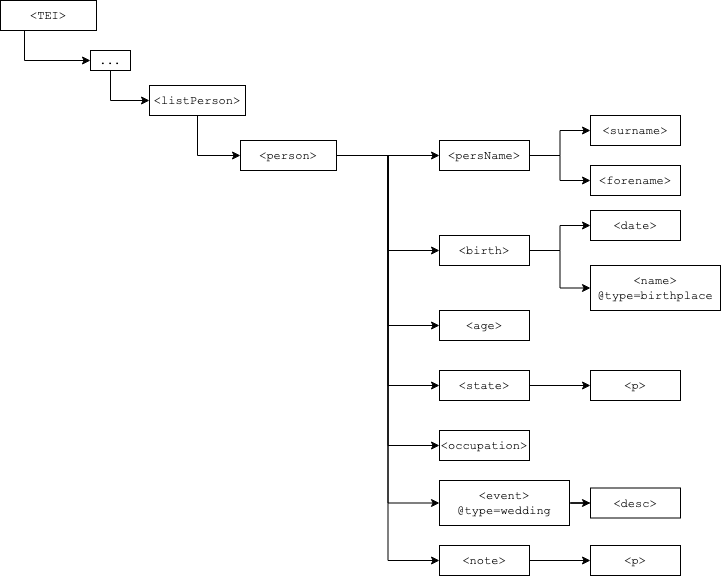
\includegraphics[width=16cm]{img/index_tree.png}
    \caption{Arbre XML simplifié montrant l'organisation d'une entrée d'index.}
    \label{fig:index_tree}
\end{figure}

\section{Indexer les individus}


Cette défaillance dans la détection des entités nommées pose problème dans la mesure où les monographies de familles prennent pour sujet un groupe d'individus (les enquêtés) sur un territoire précis ; si leurs noms sont souvent anonymisés (\textit{M***}, \textit{F***}, etc.), les prénoms sont écrits en toute lettre.

Un projet de recherche mené par le CMH et le CHR concerne ces enquêtés et souhaite les indexer en relevant les informations biographiques données par les monographes. Ce travail d'indexation des familles enquêtées est mené par Alain Cottereau et Stéphane Baciocchi (CRH, EHESS), avec Anne Lhuissier (CMH, INRAE). Ils  cherchent notamment à lever l'anonymat  des individus et à compléter (voire corriger) les informations biographiques délivrées dans les monographies, grâce à l'exploitation des fonds d'archives départementaux ou municipaux.

Anne Lhuissier et Stéphane Baciocchi se sont ainsi rendus aux Archives départementales de l'Isère pour trouver des informations sur le gantier Théodore  G., sujet principal de la monographie \no{} 55\footcite{mono055a}. Théodore  G. est présenté comme un gantier vivant à Biviers, à 9km de Grenoble. Son père, mort avant le début de l'enquête, était un riche cultivateur ; les frères de Théodore cultivent toujours, au moment de l'enquête, les terres familiales. Le monographe explique que Théodore, doté \og d'une forte constitution \fg{}, a lui-même \og pris part jusqu'à l'âge de vingt-cinq ans aux travaux de l'agriculture \fg{}\footcite[p. 471]{mono055a}.

Son service militaire l'amène ensuite à participer au siège de Sébastopol lors de la guerre de Crimée en 1855\footcite[p. 471]{mono055a}. Cependant, son père \og l'a racheté et rappelé auprès de lui \fg{}, \cad{} qu'il a payé un remplaçant qui a effectué la fin de son service militaire à sa place\footcite[p. 471]{mono055a}. C'est alors que, en dépit du fait qu'il \og passait à juste titre pour un des ouvriers les plus intelligents et les plus certains de réussir \fg{} dans l'agriculture, relate le monographe, \og il n'a pu résister au désir d'apprendre la profession de gantier \fg{}\footcite[p. 471]{mono055a}. Théodore est ainsi le seul homme de sa fratrie à ne pas être devenu agriculteur.

Or Anne Lhuissier et Stéphane Baciocchi, en exploitant les archives des séries \textsc{e} (archives notariales), \textsc{p} (cadastre) et de la sous-série \textsc{3q} (enregistrement et timbre), ont pu démontrer que Théodore avait reçu une part si faible de la succession paternelle, qu'il n'était pas envisageable pour lui de poursuivre dans l'agriculture. Ses frères avaient en effet fait valoir que le paiement d'un remplaçant pour son service militaire devait être considéré comme une avance sur l'héritage, et donc déduit de celui-ci. Théodore n'a reçu aucune partie des terres paternelles mais seulement une maison ; Anne Lhuissier et Stéphane Baciocchi font l'hypothèse que cette absence de terre à cultiver a été déterminante dans sa volonté de devenir ouvrier et donc de rompre avec le travail traditionnel de sa famille\footnote{Ces lignes sont écrites avec l'aimable autorisation d'Anne Lhuissier et de Stéphane Baciocchi ; leurs conclusions, encore inédites, devraient donner lieu à une prochaine publication.}. Cet exemple illustre les possibilités de valorisation que le programme \timeus{} envisage pour les enquêtés des \odm.

Une tableau prosopographique au format CSV était déjà établi au moment de notre stage. Huit cent quarante-deux individus y étaient identifiés et décrits selon leur état civil et des critères sociaux. Les chercheurs et les chercheuses nous ont demandé de procéder, dans un premier temps, à la transformation de ce tableau en un  index XML et, dans un second temps, à la liaison entre chaque entrée et l'individu correspondant dans les monographies (\ann{} \ref{ann:feuille_route}, \issue{} 4). Du point de vue de l'ingénierie, cela se traduisait par la constitution automatique de l'index puis par l'implémentation dans les fichiers TEI des identifiants des individus cités dans le deuxième paragraphe.

Un fichier d'index au format XML repose sur un \texttt{<body>} dans lequel une ou plusieurs listes de personnes (\texttt{<listPerson>}) sont établies, les individus y étant indexés au sein d'éléments \texttt{<person>}. Nous avons constitué une liste de personnes unique, car aucun besoin particulier ne nous a été transmis quant à cette fonctionnalité de la TEI. On pourrait néanmoins imaginer des listes en fonction des sexes et, à l'intérieur de celles-ci, des sous-listes relatives aux rôles sociaux des individus. 

Nous nous sommes concentrés sur les différentes catégories à faire figurer dans l'index et sur les balises pouvant les traduire (\fig{} \ref{fig:index_tree}).

L'identifiant de l'individu --- formé de celui de la monographie, de la lettre \textit{E} pour \textit{enquêté} et du numéro d'apparition --- constitue la valeur de l'attribut \texttt{xml:id} de la balise \texttt{<person>}. L'état civil se trouve ensuite dans un ensemble \texttt{<persName>} où le nom figure dans \texttt{<surname>} et le prénom dans \texttt{<forename>}.

D'autre balises pourraient venir compléter cette section, notamment \texttt{<addName>} pour les surnoms ou les prénoms surnuméraires. Une reprise du tableau serait néanmoins nécessaire pour rendre l'usage de cet élément possible : dans l'état actuel, le surnom ou le second prénom se trouvent dans la même cellule que le prénom, ici entre parenthèses, là après un tiret et ailleurs introduits par le transitif \textit{dit}. Une telle reprise, consistant donc à répartir en trois cellules (prénom, prénom surnuméraire, surnom) les informations contenues en une pourrait être réalisée sur la plate-forme \textit{Dataiku} qui permet la manipulation de données à grande échelle, par exemple grâce à des expressions régulières.

Les informations de naissance (date et lieu) sont placées dans un ensemble \texttt{<birth>}, suivi de l'âge (\texttt{<age>}).

La situation matrimoniale est décrite par la balise \texttt{<desc>} dans un ensemble \texttt{<event>} (évènement). La TEI conseille de décrire l'évènement de manière normalisée par un \texttt{<label>} placé avant \texttt{<desc>}. Cependant, dans la mesure où cet index ne compte qu'un seul évènement, nous avons choisi de simplifier la structure et d'en préciser la nature grâce à un attribut \texttt{@type} au niveau de \texttt{<event>}. Suivent deux indicateurs contenant le positionnement de l'individu dans la cellule familiale (\texttt{<state>} : chef de famille, femme, fille) et son activité, qu'il s'agisse d'un apprentissage, d'un métier ou d'un travail à la tâche ou à la journée (\texttt{<occupation>}). Dans une \texttt{<note>} finale figurent la date de référence pour les calcules des dates de naissance et de mariage et le rappel du titre de la monographie où apparaît l'individu.

\section{Corriger les transcriptions ?}

Dans chaque volume, le paragraphe \og État civil de la famille \fg{} commence par une liste standardisée des membres de la famille. Les figures \ref{fig:mono-56-page-4} et \ref{fig:mono-56-page-4-code} montrent une comparaison entre le texte d'origine de la monographie 56, sa transcription et son encodage par \lse\footcite[p. 4]{mono056a}. Les erreurs concernant la reconnaissance des entités nommées y apparaissent clairement : sur quatre prénoms, tous sont transcrits avec une distance d'édition importante et le nom de famille \og B*** \fg{} n'est absolument pas reconnu.

\begin{figure}[h]
    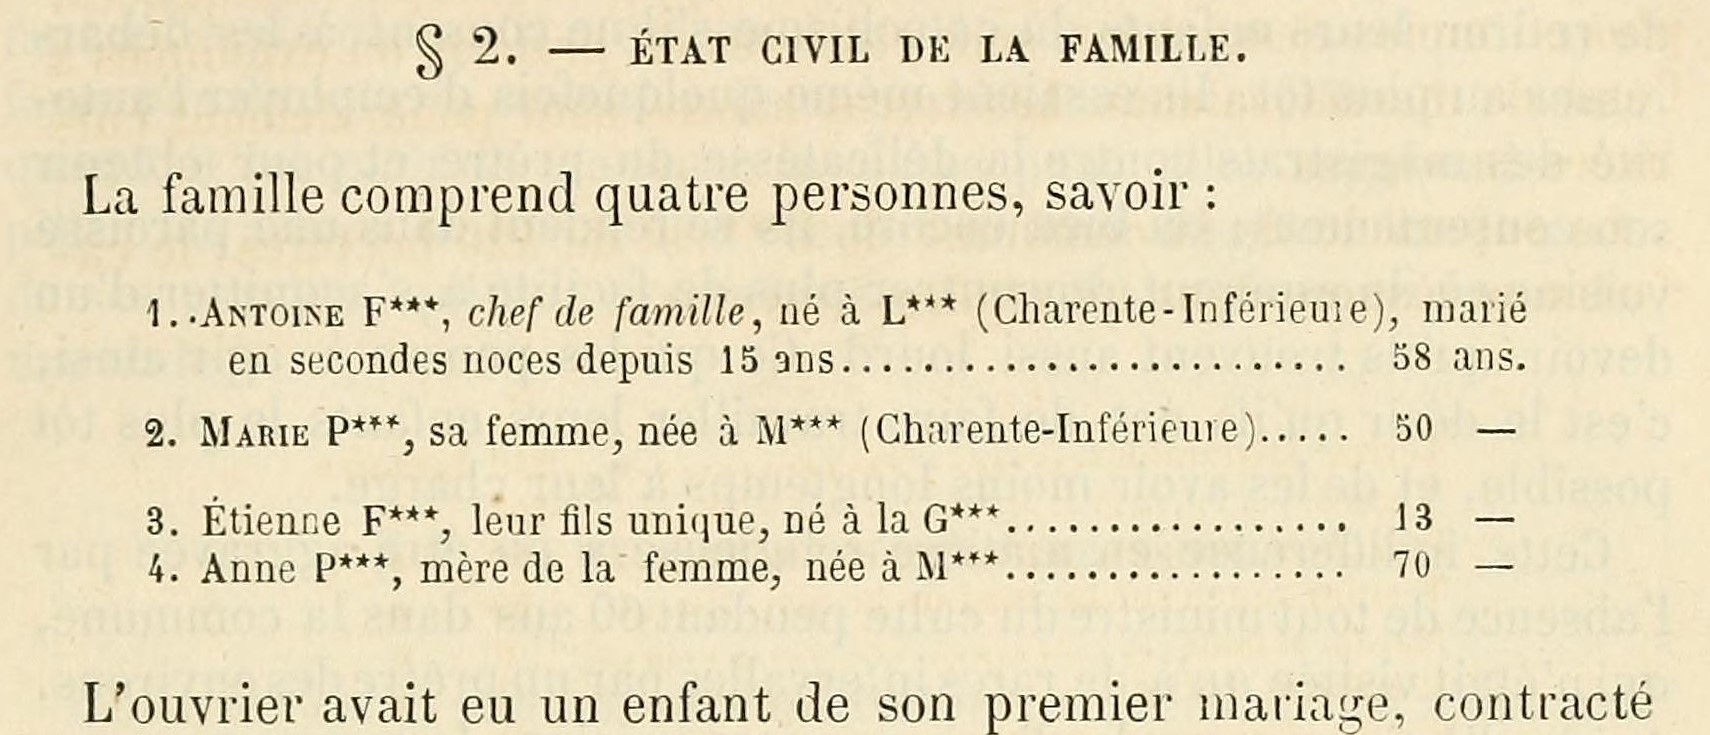
\includegraphics[width=14cm]{img/mono-23-page-209.jpg}
    \caption[Liste d'individus au début du paragraphe 2 (\no{} 23)]{Liste d'individus et son encodage (série 1, volume 3, monographie \no{} 23, page 209).}
    \label{fig:mono-23-page-209}
\end{figure}

\begin{figure}[h]
    \centering
    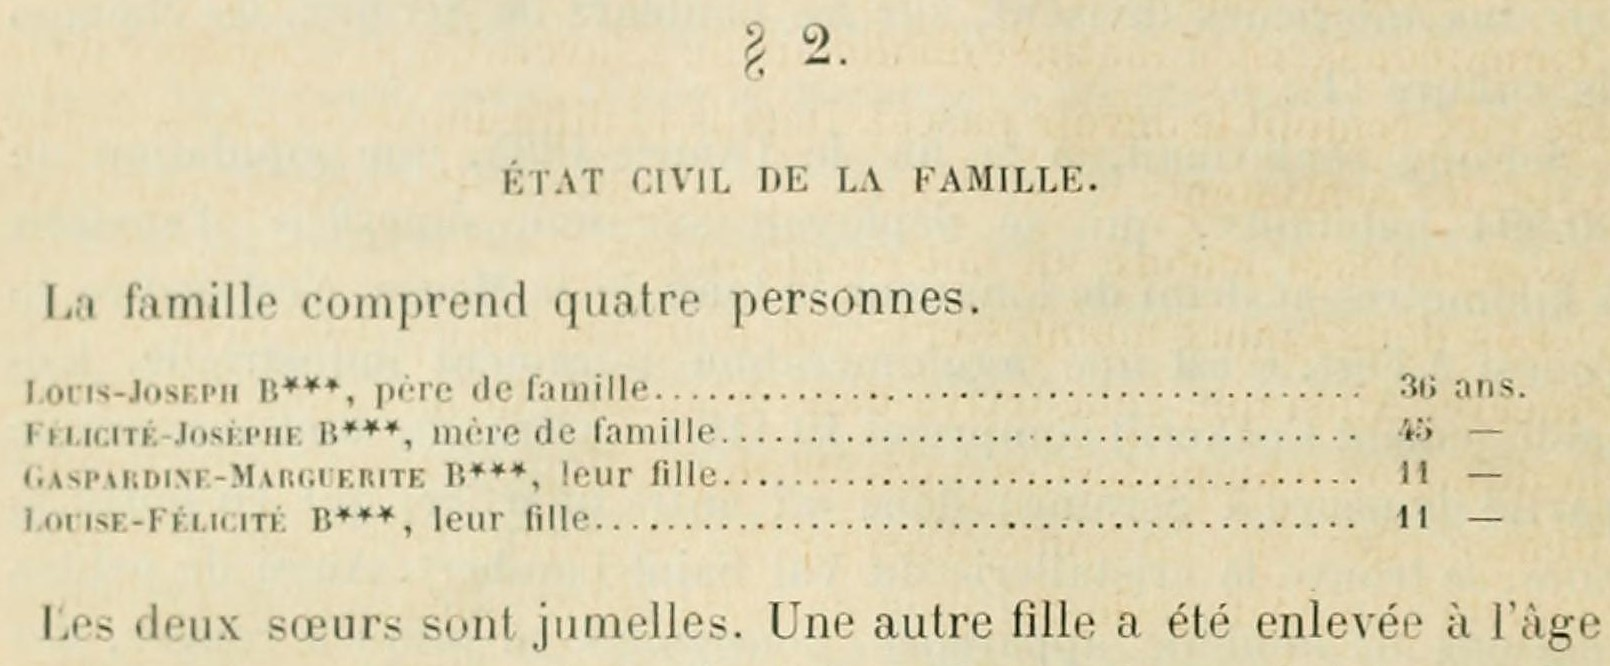
\includegraphics[width=14cm]{img/mono-56-page-4.jpg}
    \caption[Liste d'individus au début du paragraphe 2 (\no{} 56)]{Liste d'individus (série 2, volume 2, monographie \no{} 56, page 4).}
    \label{fig:mono-56-page-4}
\end{figure}

\begin{figure}[h]
    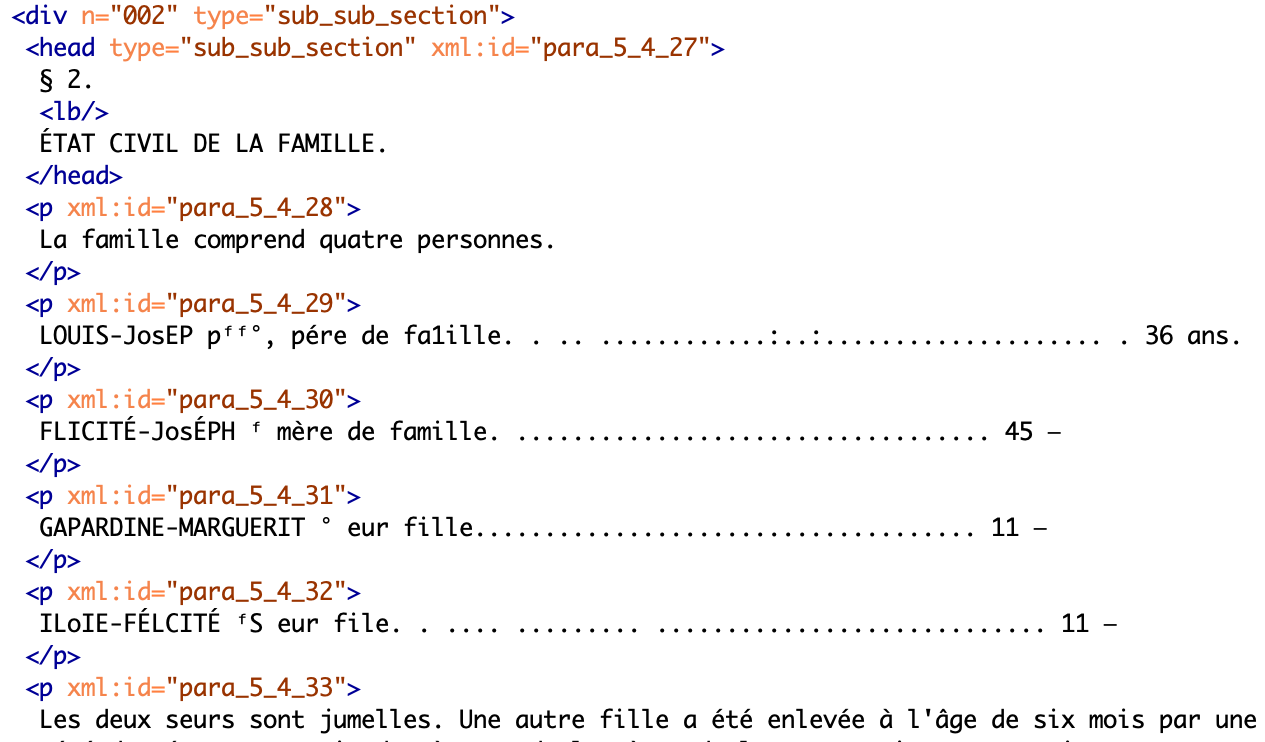
\includegraphics[width=14cm]{img/mono-56-page-4-code.png}
    \caption[Encodage de la liste d'individus (\no{} 56)]{Encodage de la liste d'individus, monographie \no{} 56 (\texttt{s2t2\_chapt\_5.xml}).}
    \label{fig:mono-56-page-4-code}
\end{figure}

Ici, ces erreurs ne posent pas qu'un problème de compréhension : elles empêchent la réalisation de la deuxième mission qui nous avait été confiée et qui consistait à lier les individus à leurs identifiants. En effet, cette opération se serait normalement traduite par l'implémentation d'une balise \texttt{<persName>} autour de chaque ensemble prénom et nom, avec un attribut \texttt{@ref} ayant pour valeur l'identifiant donné dans le fichier d'index.

L'implémentation automatique aurait pu s'effectuer de plusieurs manières, et notamment par la recherche du prénom : cela n'est pas possible du fait des distances d'édition trop grandes. Certaines monographies présentent également des listes numérotées (\fig{} \ref{fig:mono-23-page-209}) : là encore les numéros auraient pu être utiles, si seulement ils avaient été convenablement détectés.

\bigbreak

Une autre solution aurait procédé de l'observation que, les paragraphes deuxièmes commençant toujours par une phrase de type \og La famille comprend X personnes \fg{}, \og La famille comprend \fg{} ou \og Les membres de la famille sont \fg{}, les lignes qui suivent correspondent aux membres de la famille. Il eut été dès lors possible, grâce à l'ordre d'apparition noté dans le CSV, de considérer que la première de ces lignes est celle du premier individu, et ainsi de suite. Ce procédé repose cependant sur l'idée que les items des listes se trouvent sur une seule ligne, ce qui n'est pas toujours le cas (\fig{} \ref{fig:mono-23-page-209}). Du reste, placer une balise \texttt{<persName>} sur l'ensemble d'une ligne serait revenu à corrompre son usage, normalement réservé à \og un nom propre ou une expression nominale se référant à une personne \fg{}\footnote{\textit{TEI element persName (personal name)}, \textit{TEI Guidelines}.}.

Ainsi, dans tous les cas, la réalité des transcriptions empêchait l'implémentation automatique de la balise et nous confinait à une opération de correction.  Or celle-ci ne peut pas être menée sans une intervention humaine, qu'elle soit entièrement manuelle ou semi-automatisée grâce à un logiciel de suggestion de correction\footcite[p. 1]{sagot}. Ces logiciels --- par exemple, \textit{Antidote}\footnote{Présentation : \url{https://www.antidote.info/fr/} (consulté le \today).} --- s'appuient sur un lexique et, \og pour chaque mot inconnu, [cherchent] des candidats proches (par exemple en termes de distance d’édition) qui figurent dans le lexique et choisissent en prenant en compte la fréquence des candidats, le contexte, ou éventuellement un poids associé au type d’erreur présumé \fg{}\footcite[p. 1-2]{sagot}. Une telle intervention, quels que soient les moyens choisis pour sa réalisation, serait possiblement très longue et dans tous les cas coûteuse\footcite[p. 14]{en-tal}.


\begin{table}
\begin {center}
    \begin{tabular}{|c|c|c|}
\hline
    \textbf{Vérité terrain} & \textbf{\ocr} & \textbf{Correction} \\ \hline
    \textsc{Louis} & LOUIS & --- \\ \hline
    \textsc{Joseph} & JosEP & joseph \\ \hline
    \textsc{Félicité} & FLICITÉ & félicité \\ \hline
    \textsc{Josèphe} & JosÉPH & joseph \\ \hline
    \textsc{Gaspardine} & GAPARDINE & gagarine \\ \hline
    \textsc{Marguerite} & MARGUERIT & marguerite \\ \hline
    \textsc{Louise} & ILoIE & loin \\ \hline
    \textsc{Félicité} & FÉLCITÉ & félicité \\ \hline
    \end{tabular}
\caption{\label{tabl:pyspellchecker-1} Comparaison entre la vérité terrain, la transcription effectuée par l'\ocr{} et la proposition de correction de \texttt{pyspellchecker} pour les prénoms de la monographie \no{}~56 (série~2, volume~2, page~4 --- \texttt{s2t2\_chapt\_5.xml}).}
\end {center}
\end{table}

Nous nous sommes donc intéressés à la librairie Python \texttt{pyspellchecker}\footnote{Déposé sur \github{} :\url{https://github.com/barrust/pyspellchecker} (consulté le \today).}. Elle utilise un lexique, dont l'utilisateur spécifie la langue, et la distance de Levenshtein pour identifier des cacographies et proposer, selon les paramètres, soit une correction soit plusieurs candidats. La méthode \texttt{.unknown{}} affiche les mots du texte analysé qui ne se trouvent pas dans le lexique, et \texttt{.known()} ceux qui s'y trouvent\footnote{\texttt{Pyspellchecker} ne permet pas que de faire des corrections orthographiques ; en affichant les mots connus avec \texttt{.known()}, l'utilisateur peut calculer leur fréquence grâce à la méthode \texttt{.word\_probability()}.}. \texttt{Pyspellchecker} analyse ensuite les mots faux et peut, selon les paramètres, proposer une solution unique grâce à la méthode \texttt{.correction()} ou un choix entre plusieurs candidats grâce à la méthode \texttt{.candidates()}.  Par défaut, la distance est de \texttt{2}, elle peut être ramenée à \texttt{1}. Cela signifie que selon la valeur de la propriété \texttt{distance}, la librairie va considérer qu'une ou deux opérations de suppression, de substitution ou d'insertion ont pu avoir lieu.

Un test sur les cinq premiers \texttt{<p>} de la figure \ref{fig:mono-56-page-4-code} a donné de bons résultats (tabl. \ref{tabl:pyspellchecker-1}). Le script en question extrait le texte des balises \texttt{<p>} grâce à la librairie \texttt{BeautifulSoup} et le nettoie en enlevant les signes de ponctuation. Ces derniers induisent en effet le correcteur en erreur : un mot suivi d'un point sera ainsi considéré comme un seul ensemble et jugé faux\footcite[p. 60]{chiffoleau}. Le correcteur analyse ensuite chaque mot et retourne les mots faux ; nous l'avons paramétré de manière à ce qu'il propose une correction et des candidats de correction.

Le tableau \ref{tabl:pyspellchecker-1} montre que, sur sept transcriptions fausses, \texttt{pyspellchecker} permet d'en corriger quatre de manière exacte (\textit{Félicité} à deux reprises, \textit{Joseph} et \textit{Marguerite}). La vérité terrain est presque approchée pour \textit{Josèphe} : le \textit{e} final et l'accent grave manquent. En revanche, lorsque le même test est effectué sur une monographie où les prénoms ne se trouvent pas forcément dans un lexique français, par exemple la \no{} 25 consacrée à un parfumeur du bazar El Attharin-el-kebar de Tunis\footcite{mono025a}, le taux chute à un prénom corrigé sur sept erreurs (tabl. \ref{tabl:pyspellchecker-2}). La graphie de la vérité terrain \textit{Aïcha} figure bien dans la liste des candidats, mais c'est la forme \textit{Aisha} qui est choisie comme correction. On voit également que le dernier prénom, \textit{Kouka}, est transcrit avec une distance d'édition si importante (\textit{oul}, soit trois suppressions et une insertion) qu'il est improbable que le script puisse trouver le mot d'origine.

\begin{table}
\begin {center}
    \begin{tabular}{|c|c|c|}
\hline
    \textbf{Vérité terrain} & \textbf{\ocr} & \textbf{Correction} \\ \hline
    \textsc{Mohammed} & MloAMMED & mohammed \\ \hline
    \textsc{Kadidja} & bADIDJA & badidja \\ \hline
    \textsc{Rhkeïma} & Rhleima & rhleima \\ \hline
    \textsc{Ahsoûn} & Ahsoùn & ahsoka \\ \hline
    \textsc{Aïcha} & Aicha & aisha \\ \hline
    \textsc{Arouçi} & AroOuci & adouci \\ \hline
    \textsc{Kouka} & oul & oui \\ \hline
    \end{tabular}
\caption{\label{tabl:pyspellchecker-2} Comparaison entre la vérité terrain, la transcription effectuée par l'\ocr{} et la proposition de correction de \texttt{pyspellchecker} pour les prénoms de la monographie \no{}~25 (série~1, volume~3, page~286 --- \texttt{s1t3\_chapt\_10.xml}).}
\end {center}
\end{table}

Si ce test pourrait être transformé en un script d'aide à la correction, la présence d'un opérateur humain pour valider ou non les propositions de \texttt{pyspellchecker} reste indispensable. C'est la méthode utilisée par Floriane Chiffoleau (prom. 2019) lors de son stage de fin d'étude au sein du projet MetaLEX de l'EHESS, dont l'objectif est \og d’élaborer un système d’informations métalexicographiques,
concernant le vocabulaire portant sur les langues historiques du droit en Europe \fg\footcite[p. 9]{chiffoleau}. Elle a plus précisément travaillé sur l'édition numérique du \textit{Dei Delitti e delle Pene} de Cesare Beccaria (1764), ce qui l'a conduit à utiliser \texttt{pyspellchecker} pour corriger les résultats de son \ocr. Elle produit dans son mémoire un retour d'expérience détaillé sur l'utilisation de cette librairie, en insistant sur la division des tâches et la constitution de dictionnaires Python\footcite[chap. 8, \textit{Établir une correction orthographique et une annotation linguistique semi-automatique}, p. 57-66]{chiffoleau}.

Cinq étapes sont décrites. La première consiste à nettoyer et mettre en forme automatiquement le texte en supprimant les sauts de ligne, les espaces en trop et les signes de ponctuation\footcite[p. 54 et 60]{chiffoleau}. Les erreurs sont ensuite relevées par \texttt{pyspellchecker} et réparties en trois ensembles : une liste avec les mots non-reconnus mais justes, un dictionnaire Python avec les versions non-usuelles du \textsc{xvii}\ieme~siècle (par ex. \textit{paroître} à la place de \textit{paraître}\footcite[p. 57]{chiffoleau}) et un dernier dictionnaire contenant les erreurs véritables et leurs corrections\footcite[p. 59-60]{chiffoleau}. Lors de la troisième étape, le texte est cette fois-ci récupéré en entier, avec sa mise en forme et sa ponctuation\footcite[p. 61]{chiffoleau}. Le dictionnaire d'erreurs est passé en revue lors de l'étape suivante afin de contrôler et d'amender si nécessaire les propositions de \texttt{pyspellchecker}\footcite[p. 61-63]{chiffoleau}. Les opérations de correction sont enfin opérées à l'aide d'une fonction de recherche et de remplacement à partir du dictionnaire d'erreurs : chaque mot faux est recherché et ses occurrences sont remplacées par sa correction\footcite[p. 63-64]{chiffoleau}.

\texttt{Pyspellchecker} a  fait ses preuves dans plusieurs projets de recherche : MetaLEX, comme nous venons de le voir, mais également DAHN pour lequel Floriane Chiffoleau travaille aujourd'hui en tant qu'ingénieure de recherche et de développement de l'équipe ALMAnaCH. Son expérience et ses scripts peuvent être ré-utilisés pour les fichiers des \odm{}, avec quelques modifications dues notamment au fait que nos fichiers ne contiennent pas de mots en ancien français\footnote{Les scripts utilisés par Floriane Chiffoleau lors de son stage sont déposés sur \github{} : \url{https://github.com/FloChiff/memoire-M2/tree/master/Livrable\%20technique/Scripts/2\%20-\%20Nettoyage\%20de\%20texte} (consulté le \today).}. Nous pouvons également observer que la majorité du processus est automatisé, mis à part la correction du dictionnaire d'erreurs.

Une autre librairie Python, \texttt{pygrammalecte}, peut être utilisée pour générer un rapport d'identification des erreurs. La différence avec la librairie précédente est qu'elle fonctionne avec un dictionnaire et est capable, en plus de détecter les erreurs, de les répartir dans une typologie (orthographe, grammaire, ponctuation). Cette librairie est utilisée par le service humanités numériques de l'École nationale des chartes pour évaluer la qualité des \ocr{} des positions des thèses pour le diplôme d'archiviste paléographe, et permet de générer un rapport d'erreur sous la forme d'un fichier JSON\footnote{Voir notamment la fonction \texttt{ocrquality} dans le script \texttt{encpos\_control.py}, ligne 72 : \url{https://github.com/chartes/encpos/blob/38ad0277a03467642dd8a329a37237c9e663f4d1/utils/encpos_control.py\#L72} (consulté le \today).}.

On le voit, il est possible de développer des solutions en interne pour corriger une \ocr. Si elles n'automatisent pas totalement cette correction, elles permettent de réduire son coût budgétaire en épargnant le recours à un prestataire externe ou l'achat d'un logiciel dédié. Elle peuvent néanmoins se traduire par le recours à un vacataire pour le temps de la correction, ce qui représente tout de même un poste de dépense.

Durant notre stage, nous avons contourné le problème en ajoutant, au début des deuxièmes paragraphes, un commentaire contenant les identités des individus cités et leurs identifiants. Un commentaire est dans un fichier informatique une section du code destinée à la lecture par un humain et non par une machine, qui de fait l'ignore au moment de l'interprétation du fichier. En XML, le commentaire est délimité par les symboles \texttt{<!--} et \texttt{-->}. Dans la monographie \no{} 56, cela donne cette ligne :

\begin{quote}
    \texttt{<!-{}- Individus cités : Louis-Joseph B*** (\no{}056aE1) - Félicité-Josèphe B*** (\no{} 056aE2) - Gaspardine-Marguerite B*** (\no{} 056aE3) - Louise\-Félicité B*** (\no{} 056aE4) -{}->}
\end{quote}

Il s'agit d'une solution d'attente qui n'a pas vocation à demeurer dans la version définitive des fichiers.

\chapter{Une valorisation plurielle}

\section{Édition papier, édition numérique}

Un postulat commun veut qu'une édition numérique offre à son utilisateur plus de possibilités qu'une édition papier n'en offre à son lecteur\footnote{\og \textit{Often these descriptions glance at their print predecessors, usually with expressions of how much more these digital editions can contain than ever could be included in print editions, and how much more the reader can do with them} \fg{} : \cite[p. 105-106]{robinson}.}. Le numérique permet en effet de concevoir des plate-formes sur mesure pour la consultation des textes, et les outils des humanités numériques permettent à \og de nombreuses données non interrogeables jusqu’à présent [d'être] l’objet d’enquêtes \fg\footcite[p. 20]{duval}. \og Des structures cachées, des faits de système difficilement décelables à l’œil et à la main \fg{} deviennent ainsi accessibles\footcite{duval}.

Dans le programme \timeus{}, l'édition numérique des \odm{} a éveillé l'intérêt d'au moins trois participants. Le LARHRA de l'université de Lyon 2, dans le strict respect des objectifs du programme, souhaite utiliser les informations économiques fournies par les tableaux de budget et celles d'ordre prosopographique contenues dans le paragraphe \og §2 --- État civil de la famille \fg. L'équipe ALMAnaCH d'Inria a pour sa part la volonté de puiser dans les champs lexicaux des mondes ouvrier et industriel afin d'alimenter des algorithmes de traitement automatique du langage (TAL). Enfin, le Centre de recherches historiques (CRH) veut fournir à la communauté scientifique une édition numérique des \odm{} qui intégrerait des informations matérielles sur la constitution du corpus et le travail de la \sess.

On le voit, les objectifs poursuivis par ces entités sont très divers. Les matériaux qui permettront de les réaliser le sont tout autant : le LARHRA et ALMAnaCH ont besoin de données brutes issues des tableaux statistiques (des chiffres) et du texte (des mots), tandis que le CRH agrège des métadonnées inédites qui proviennent de plusieurs corpus ; il dispose notamment d'un exemplaire des deuxième et troisième séries encore à l'état de fascicules non reliés. Le LARHRA a également besoin d'une transcription de qualité pour s'assurer de la viabilité des informations prosopographiques du second paragraphe.

Cette pluralité de directions illustre la tension qui traverse les éditions numériques : elles portent avant tout sur un document et non sur une \oe{}uvre\footnote{\og \textit{Two decades of making digital editions, and recent papers about digital editions, have moved the needle away from the “work” to the “document”, to the point where we might need only think of “documents”} \fg{} : \cite[p. 107]{robinson}}. Cette distinction est issue de la triade document, texte, \oe{}uvre (\textit{document}, \textit{text}, \textit{work}) qui désigne les dimensions matérielle, linguistique et intellectuelle d'un écrit\footnote{\og \textit{Work} désigne le texte de l’auteur, éventuellement le texte correspondant à la volonté de l’auteur, et implique la notion d’authenticité ; \textit{text} dénomme la séquence linguistique attestée dans un document transmettant l’œuvre ; enfin \textit{document} est une manifestation physique d’un text \fg{} : \cite[p. 15-16]{duval}.}. De fait, l'encodage que nous avons décrit dans la partie précédente fait la part belle au document \odm{} de l'Université de Toronto, digitalisé par \ia. \transkribus{} et le script \lse{} mobilisent la TEI pour conduire sa reproduction fidèle grâce à des ensembles \texttt{<facsimile>}\footcite[p. 124]{robinson}. L'\oe{}uvre n'est pas pour autant oubliée. Elle se rencontre dans la structure logique leplaysienne, là encore reproduite fidèlement par le biais des divisions et des titres.

Cette coexistence apparente et inégale n'a cependant pas vocation à durer : dans la vision de \timeus, c'est bien l'\oe{}uvre et non le document qui doit prendre le dessus. Il n'est pas question de concevoir un support de consultation qui présenterait des échantillons successifs correspondant au contenu d'une page. Cela reviendrait à reproduire l'interface de visualisation d'\ia, tout en donnant une réalité concrète à l'hypertexte qui est \og en gestation dans les tables, index et diverses aides à la lecture de consultation déjà présentes \fg{} dans les volumes\footcite[p. 19]{duval}.

Ces observations montrent qu'une édition numérique se doit d'être équilibrée et de rendre compte à la fois du document-texte et de l'\oe{}uvre-texte\footnote{\og \textit{A scholarly edition must, so far as it can, illuminate both aspects of the text, both text-as-work and text-as-document} \fg{} : \cite[p. 123]{robinson}.}, sans quoi elle risque de perdre tant ses lecteurs\footnote{\og \textit{But there are dangers here. (...) Facsimile editions in print form are of very little use to the reader, or even to scholars, whose interest (...) is likely to be in questions of how the received text changed over time, how it was received, how it was altered, transformed, passed into different currencies. If we make only digital documentary editions, we will distance ourselves and our editions from the readers} \fg{} : \cite[p. 127]{robinson}.} que ses utilisateurs\footnote{\og La lisibilité des éditions électroniques n’a rien à envier à celle des éditions papier. (...) Parfois, les interfaces ne sont pas intuitives et requièrent une longue familiarisation ; d’autres fois, des aides à la lecture systématiquement présentes dans les éditions papier disparaissent \fg{} : \cite[p. 21]{duval}.}.

Le premier essai d'édition des fichiers XML, mené par Alix Chagué, consiste ainsi en un document HTML où l'intégralité du texte du premier volume est reproduit, organisé en fonction de la structure logique et non des zones de segmentation\footnote{Cette démonstration est visible à cette adresse : \url{http://demo-leplay.herokuapp.com/volume_parsed_test.html} (consulté le \today).}. Elle pourrait cependant être améliorée avec des informations issues du document, à commencer par la traduction, par exemple entre crochets droits, des balises \texttt{<pb>} à chaque changement de page.

\timeus{} a identifié deux voies possibles pour une publication effective. La première consiste à déposer les textes sur \wikisource. Il s'agit d'une bibliothèque numérique maintenue par la fondation Wikimédia, gratuite, en \openaccess, contenant des \opendata{} (aucune restriction sur l'usage des données) et ouverte à tous ceux qui souhaitent y contribuer. Le problème est que les fichiers XML ne peuvent pas être versés en l'état : ils doivent être modifiés voire transformés dans la syntaxe de la Wikimedia, le wikicode. Cette opération peut donc s'avérer coûteuse et le transfert de la totalité des informations n'est pas garanti ; les dépôts git sont de ce \pov{} de bien meilleures solutions.

Cependant, le principe de \wikisource{} pourrait être conservé tout en contournant les règles de sa communauté. Le CRH souhaite en effet utiliser l'un de ses wikis sémantiques, \textit{Ethnocomptabilités}, pour publier les monographies et leurs métadonnées entendues au sens large (volumes, enquêtés, enquêteurs)\footnote{\textit{Ethnocomptabilités} est hébergé à cette adresse : \url{http://ethnocompta.huma-num.fr/} (consulté le \today).}. Un wiki sémantique est un wiki --- \cad{} une application web où des pages peuvent être créées et modifiées par des utilisateurs --- augmenté de renseignements sémantiques permettant de qualifier les relations entre les pages et, \textit{in fine}, de manipuler les données qui s'y trouvent\footcite{poupeau}. Le programme \timeus{} y est libre de publier ses données sous la forme qu'il souhaite ; cette publication doit néanmoins s'accompagner d'un effort de référencement et de communication afin que le wiki soit consulté et utilisé par la recherche.

\section{Retrouver les fascicules dans le volume}

Au premier abord, il est aisé de considérer les \odm{} comme une \oe{}uvre. Mais plus on progresse dans l'histoire de cette entreprise, plus cette idée première se fragilise. En effet, si ce corpus s'incarne aujourd'hui dans des volumes, ceux-ci étaient autrefois des fascicules. Il est en outre constitué de monographies réparties en trois séries, tout en formant un ensemble cohérent dont les membres \og prennent sens les uns par rapport aux autres \fg{}\footcite[p. 5]{chenu}. D'une certaine manière, la volonté du CRH d'explorer l'histoire matérielle du corpus pour compléter les métadonnées des fichiers XML remet en question l'existence de \og l'\oe{}uvre \odm{} \fg{}.

Les enjeux de l'édition numérique d'un texte imprimé aux \textsc{xix}\ieme{} et \textsc{xx}\ieme~siècles divergent de ceux sous-entendus par l'édition de texte imprimé lors de siècles antérieurs. Aucune ré-impression n'est ici attestée : le texte est le même d'un exemplaire à l'autre, et ce jusque dans ses imperfections. C'est la raison pour laquelle l'encodage ne fait aucun effort de lématisation et qu'il s'appuie, de fait, sur les seules numérisations des exemplaires de Toronto.

Dans l'encodage d'un texte imprimé tel que \lodm{}, le défi se situe non pas au niveau du texte et de ses différentes versions, mais bien dans la restitution de la génétique matérielle qui a amené à la constitution des volumes. Comment traduire dans l'encodage les stratégies mises en place par les différents relieurs pour fondre les fascicules dans le volume ? Dans les exemplaires de la Bibliothèque nationale de France, les feuillets liminaires des fascicules ont été placés après les tables, là où ailleurs ils ont été conservés dans le flux du texte. Il y a ici une subtilité dont l'encodage de niveau \og document \fg{} ne se préoccupe pas, et qui pourtant est essentiel pour les deux autres niveaux.

Les observations relevées par le CRH peuvent être insérées dans la partie \texttt{<sourceDesc>} du \texttt{<teiHeader>}. Le document encodé y est décrit dans une section \texttt{<msDesc>}, où une unité codicologique distincte de l'unité documentaire principale peut être elle-même décrite grâce à la sous-section \texttt{<msPart>} (\fig{} \ref{fig:tree_msDesc}).

\begin{figure}
    \centering
    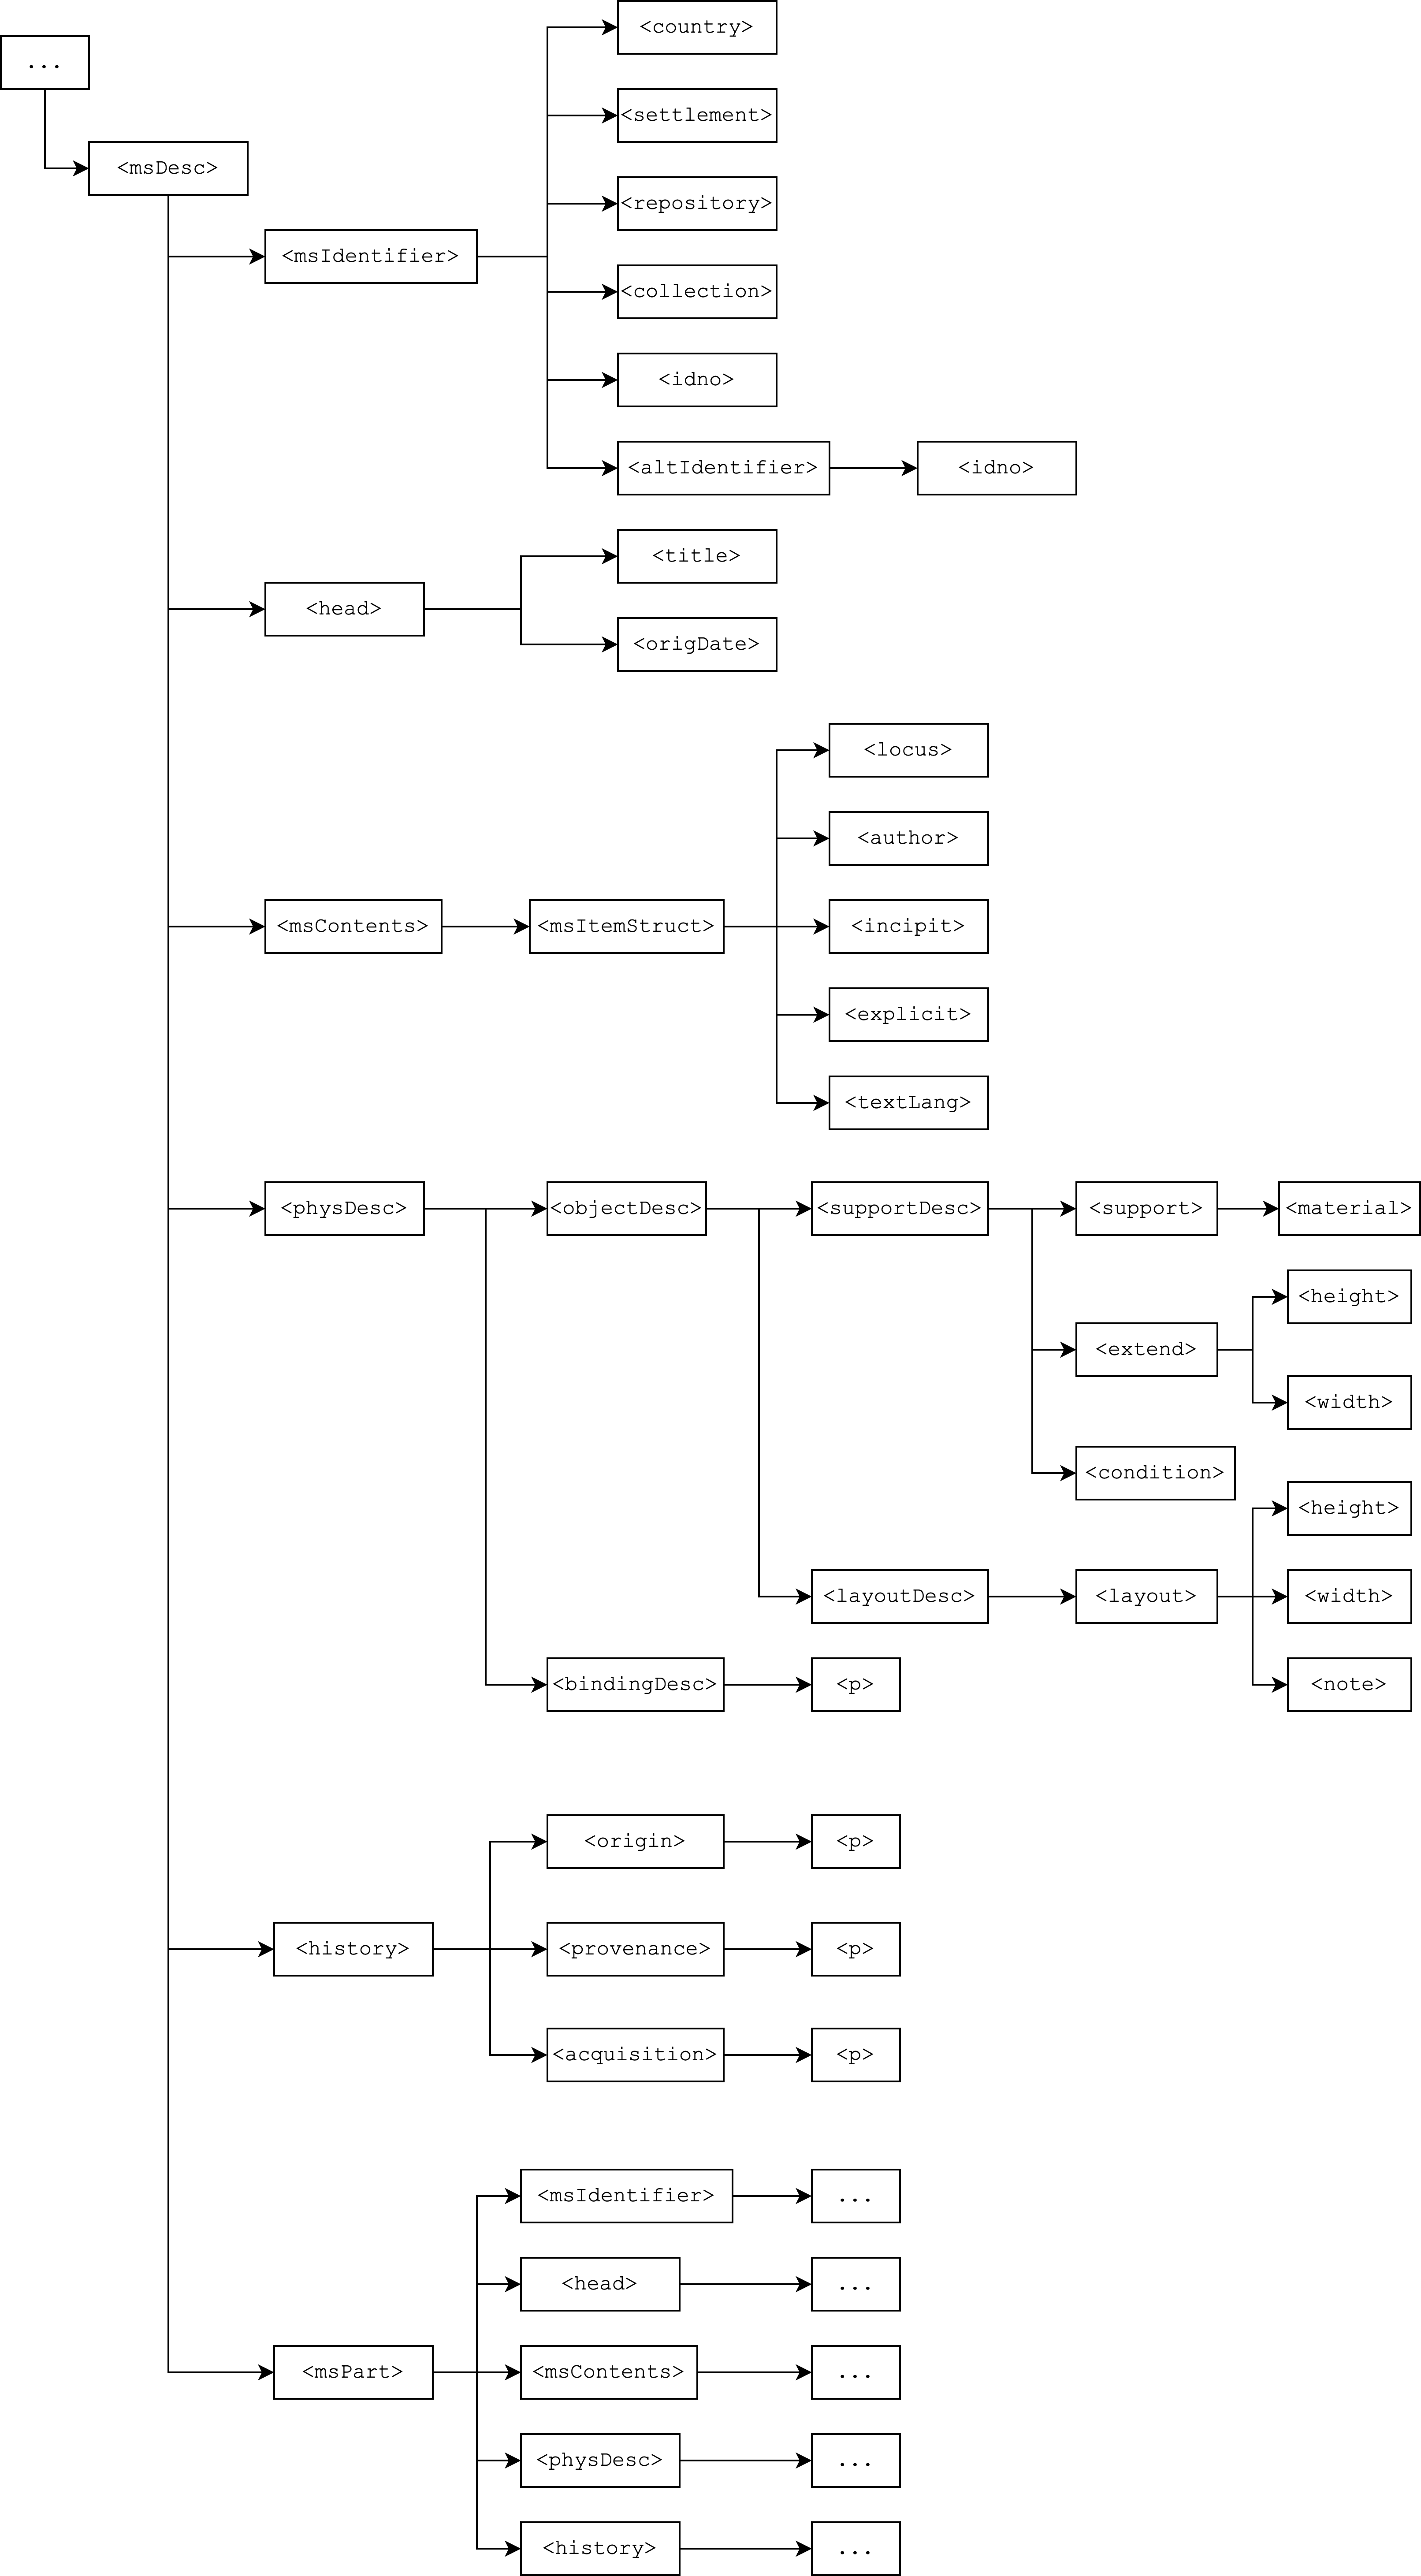
\includegraphics[scale=0.625]{img/tree_msDesc.png}
    \caption{Représentation de la section \texttt{<msDesc>} du \texttt{<teiHeader>}.}
    \label{fig:tree_msDesc}
\end{figure}

Plusieurs types de métadonnées sont spécifiés dans le \texttt{<msDesc>}. Le volume est tout d'abord identifié dans le \texttt{<msIdentifier>} par l'exposé de ses situations géographique (pays et ville de conservation) et institutionnelle (institution et département de conservation, cote), et la liste de ses copies, telles que la numérisation sur \ia. Il est ensuite titré et daté dans une partie \texttt{<head>}, avant que le \texttt{<msContents>} ne donne des informations sur sa structure : l'auteur, la pagination, la langue, l'\textit{incipit} et l'\textit{explicit}. Les caractéristiques physiques sont ensuite inscrites dans le \texttt{<physDesc>} (support, dimensions, mise en page, état). La reliure du volume et les marbrures des gardes sont décrites dans le \texttt{<bindingDesc>}.

L'histoire du volume est enfin détaillée dans la partie \texttt{<history>}, grâce à des éléments sur son origine (contexte d'édition), sa provenance (évènements entre l'origine et l'acquisition) et son acquisition (contexte d'acquisition). La pertinence d'une telle partie n'est pas certaine, tant pour les \odm{} que pour le corpus de fascicules non-reliés à la disposition du CRH et du CMH, car leurs histoires ne sont pas connues. Quelques relevés peuvent permettre d'éclaircir des points très spécifiques, par exemple la dédicace d'un monographe dans le volume 5\footnote{\og M. Auguste Moussel, hommage en cordial confraternité. Urbain Guérin \fg{} : \cite{mono083a}.}.

Le \texttt{<msDesc>} se conclurait par un \texttt{<msPart>} centré sur le fascicule, divisé selon le même plan.

Ces apports se bornent aux métadonnées, l'encodage produit par \lse{} et amélioré par notre reprise n'étant pas affecté. Rappelons que celui-ci n'est pas pour autant fixé. La place des objets graphiques reste à définir. Si la structure logique est en place, le système des renvois entre les monographies n'a pas été valorisé ; les informations prosopographiques doivent également être repérées et signalées après une correction des transcriptions.

\section{\textit{Quid} de la donnée ?}

Une question demeure au sujet des fichiers des \odm{} : quel avenir pour eux, non pas dans une mise en scène quelconque, mais en tant que données brutes ? Le choix de recourir au format XML-TEI montre que \timeus{} entend assurer la conservation des fichiers. La TEI est en effet maintenue par une communauté active. En rédigeant une cartographie du corpus et surtout une ODD, nous avons documenté la pratique éditoriale et favorisé sa compréhension par d'autres chercheurs et chercheuses ou projets qui souhaiteraient réutiliser l'encodage. Le dépôt en ligne sur le \gitlab{} de l'Inria assure la conservation de l'historique de nos interventions.

Néanmoins, le dépôt \gitlab{} est aujourd'hui en accès restreint, aussi le corpus n'est-il pas en accessible librement (\openaccess). Cette restriction est bien évidemment due au fait que le travail n'est pas achevé et sera levée à la fin du programme ANR. Pour autant, \timeus{} souhaite démultiplier les espaces de conservation en clonant le dépôt \gitlab{} sur \github. Ces deux sites offrent des services d'hébergement utilisant la technologie git, à la différence que \github{} est une entreprise commerciale possédée par Microsoft, aussi ne dépend-t-elle pas d'une institution publique dont les orientations budgétaires peuvent changer. Des procédures de migration existent entre les deux plates-formes et concernent les \commits{} comme les \issues{} et les \mergerequests.

Le CRH veut également verser les fichiers XML et peut-être, par sécurité, les images, dans l'entrepôt de données de l'EHESS, \textit{Didomena}\footnote{\textit{Le projet Didomena : une plate-forme moderne au service de la gestion des données de la recherche en sciences humaines et sociales} (\url{https://didomena.ehess.fr/informations}, consulté le \today).}. Cette application traite les données sur deux niveaux. Le logiciel \textit{Hyrax} reçoit d'abord les fichiers, les stocke et leur agrège des métadonnées dont les descriptions respectent le standard \textit{Portland Common Data Model}\footnote{Présentation accessible à \url{https://github.com/duraspace/pcdm/wiki} (consulté le \today).} ; elles sont ainsi assurées d'être interopérables. La seconde dimension est la couche applicative, soutenue par le logiciel \textit{Solr}, qui organise des vues logiques et permet des recherches à facettes dans les données comme dans les métadonnées. Le point faible est que la consultation n'est pas libre : il faut disposer d'un compte dans un établissement d'enseignement supérieur ou de recherche pour se connecter sur la plate-forme.

Ces différentes pistes montrent que les données des \odm, déjà standardisées, documentées et pérennisées, bientôt en \textit{open access}, sont assurées d'être indépendantes de toutes les mises en scène auxquelles elles pourraient se prêter\footcite[p. 63]{jolivet}.

Ces dernières années, l'écosystème de la donnée s'est néanmoins tourné vers la mise en relation de celles-ci\footcite[p. 66]{jolivet}. Une des conditions pour réaliser cela est l'interopérabilité. Les fichiers des \odm{} satisfont-ils à cette demande ? En d'autres termes, la question est de déterminer si les données qu'ils contiennent peuvent être enrichies par des informations venues d'autres formats, ou bien si elles peuvent être réutilisées par des programmes de recherche ou avec d'autres corpus dont le standard n'est peut-être pas la TEI, ou qui n'ont pas le même usage de la TEI. C'est là où le bât blesse : la TEI, du fait de son extrême souplesse, permet des pratiques éditoriales qui peuvent être très éloignées. Ce que les corpus gagnent en précision et en fidélité par rapport au(x) document(s) d'origine, ils le perdent en interopérabilité\footcite[p. 61-62]{jolivet}.

\backmatter
\part*{Annexes}
\addcontentsline{toc}{part}{Annexes}
\appendix
\renewcommand{\thechapter}{A}
\chapter{A. \lodm}

\section{Liste des monographies et fichiers correspondants}
\label{mapping}

\textit{La date de publication du volume est indiquée entre parenthèses, tandis que les dates de parution des fascicules le sont entre crochets droits.}

\subsection{Série 1, vol. 1 (1857).}
\label{mappings1t1}

URL sur \ia{} : 

\url{https://archive.org/details/lesouvriersdesde01sociuoft}.

URL sur \textit{Gallica} : 

\url{https://gallica.bnf.fr/ark:/12148/bpt6k94393f}.

\begin{center}
\begin{longtable}{ | c | p{9.5cm} | c | }
\hline
Id & Intitulé & Fichier \\ \hline
\texttt{401a} & Page de titre & \texttt{s1t1\_chapt\_1.xml} \\ \hline
\texttt{402a} & Avertissement. Considérations générales sur la Société internationale des études pratiques d'économie sociale. Son but et ses moyens d'action. & \texttt{s1t1\_chapt\_2.xml} \\ \hline
\texttt{403a} & Institution. Société internationale des études pratiques d'économie sociale. Fondation et premiers travaux. & \texttt{s1t1\_chapt\_3.xml} \\ \hline
\texttt{404a} & Définitions par ordre alphabétiques des termes à employer dans les monographies, pour désigner les ouvriers, leurs moyens d'existence, et les rapports qui les unissent soit entre eux, soit avec les autres classes. & \texttt{s1t1\_chapt\_4.xml} \\ \hline
\texttt{405a} & Explications des signes de renvoi et des abréviations. & \texttt{s1t1\_chapt\_5.xml} \\ \hline
\texttt{001a} & Charpentier de Paris (Seine - France), de la Corporation des compagnons du Devoir & \texttt{s1t1\_chapt\_6.xml} \\ \hline
\texttt{002a} & Manœuvre-Agriculteur de la Champagne pouilleuse (Marne - France) & \texttt{s1t1\_chapt\_7.xml} \\ \hline
\texttt{003a} & Paysans en communauté du Lavedan (Hautes-Pyrénées - France) & \texttt{s1t1\_chapt\_8.xml} \\ \hline
\texttt{004a} & Paysan du Labourd (Basses-Pyrénées - France) & \texttt{s1t1\_chapt\_9.xml} \\ \hline
\texttt{005a} & Métayer de la banlieue de Florence (Grand-Duché de Toscane) & \texttt{s1t1\_chapt\_10.xml} \\ \hline
\texttt{006a} & Nourrisseur de vaches de la banlieue de Londres (Middlesex - Angleterre) & \texttt{s1t1\_chapt\_11.xml} \\ \hline
\texttt{007a} & Tisseur en châles de la fabrique urbaine collective de Paris (Seine - France) & \texttt{s1t1\_chapt\_12.xml} \\ \hline
\texttt{008a} & Manœuvre-agriculteur du comté de Nottingham (Angleterre) & \texttt{s1t1\_chapt\_13.xml} \\ \hline
\texttt{009a} & Pêcheur côtier, maître de barque de Saint-Sébastien (Guipuscoa - Espagne) & \texttt{s1t1\_chapt\_14.xml} \\ \hline
\texttt{406a} & Tables alphabétique et analytique des matières contenues dans ce tome premier. & \texttt{s1t1\_chapt\_15.xml} \\ \hline
\texttt{407a} & Liste des monographies destinées aux prochaines publications de la société d'économie sociale. & \texttt{s1t1\_chapt\_16.xml} \\ \hline
\texttt{408a} & Tables des matières contenues dans ce tome premier & \texttt{s1t1\_chapt\_17.xml} \\ \hline
\end{longtable}
\end{center}

\subsection{Série 1, vol. 2 (1858).}
\label{mappings1t2}

URL sur \ia{} : 

\url{https://archive.org/details/lesouvriersdesde02sociuoft}.

URL sur \textit{Gallica} : 

\url{https://gallica.bnf.fr/ark:/12148/bpt6k943954}.

\begin{center}
\begin{longtable}{ | c | p{9.5cm} | c | }
\hline
Id & Intitulé & Fichier \\ \hline
\texttt{409a} & Page de titre & \texttt{s1t2\_chapt\_1.xml} \\ \hline
\texttt{410a} & Avertissement & \texttt{s1t2\_chapt\_2.xml} \\ \hline
\texttt{010a} & Ferblantier, couvreur et vitrier d'Aix-les-Bains (Savoie - États Sardes) & \texttt{s1t2\_chapt\_3.xml} \\ \hline
\texttt{011a} & Carrier des environs de Paris (Seine - France) & \texttt{s1t2\_chapt\_4.xml} \\ \hline
\texttt{012a} & Menuisier-charpentier (Nedjar) de Tanger (Province de Tanger - Maroc) & \texttt{s1t2\_chapt\_5.xml} \\ \hline
\texttt{013a} & Tailleur d'habits de Paris (Seine - France) & \texttt{s1t2\_chapt\_6.xml} \\ \hline
\texttt{014a} & Compositeur-typographe de Bruxelles (Brabant - Belgique) & \texttt{s1t2\_chapt\_7.xml} \\ \hline
\texttt{015a} & Décapeur d'outils en acier de la fabrique d'Hérimoncourt (Doubs - France) & \texttt{s1t2\_chapt\_8.xml} \\ \hline
\texttt{016a} & Monteur d'outils en acier de la fabrique d'Hérimoncourt (Doubs - France) & \texttt{s1t2\_chapt\_9.xml} \\ \hline
\texttt{017a} & Porteur d'eau de Paris (Seine - France) & \texttt{s1t2\_chapt\_10.xml} \\ \hline
\texttt{018a} & Paysans en communauté et en polygamie de Bousrah (Esky Cham), dans le pays de Haouran (Syrie - Empire Ottoman) & \texttt{s1t2\_chapt\_11.xml} \\ \hline
\texttt{019a} & Débardeur et piocheur de craie de la banlieue de Paris (Seine - France) & \texttt{s1t2\_chapt\_12.xml} \\ \hline
\texttt{411a} & Tables alphabétique et analytique des matières contenues dans ce tome second & \texttt{s1t2\_chapt\_13.xml} \\ \hline
\texttt{412a} & Errata & \texttt{s1t2\_chapt\_14.xml} \\ \hline
\texttt{413a} & Tables des matières contenues dans ce tome second & \texttt{s1t2\_chapt\_15.xml} \\ \hline
\end{longtable}
\end{center}

\subsection{Série 1, vol. 3 (1861).}
\label{mappings1t3}

URL sur \ia{} : 

\url{https://archive.org/details/lesouvriersdesde03sociuoft}.

URL sur \textit{Gallica} : 

\url{https://gallica.bnf.fr/ark:/12148/bpt6k633133}.

\begin{center}
\begin{longtable}{ | c | p{9.5cm} | c | }
\hline
Id & Intitulé & Fichier \\ \hline
\texttt{414a} & Page de titre & \texttt{s1t3\_chapt\_1.xml} \\ \hline
\texttt{415a} & Avertissement & \texttt{s1t3\_chapt\_2.xml} \\ \hline
\texttt{416a} & Rapport. Société d'économie sociale. Travaux de 1859-1860 & \texttt{s1t3\_chapt\_3.xml} \\ \hline
\texttt{417a} & Liste générale des membres de la Société internationale des études pratiques d'économie sociale & \texttt{s1t3\_chapt\_4.xml} \\ \hline
\texttt{020a} & Brodeuses des Vosges (Vosges - France) & \texttt{s1t3\_chapt\_5.xml} \\ \hline
\texttt{021a} & Paysan et savonnier de la Basse-Provence (Bouches-du-Rhône - France) & \texttt{s1t3\_chapt\_6.xml} \\ \hline
\texttt{022a} & Mineur des Placers du comté de Mariposa (Californie - États-Unis) & \texttt{s1t3\_chapt\_7.xml} \\ \hline
\texttt{023a} & Manœuvre-vigneron de l'Aunis (Charente-inférieure - France) & \texttt{s1t3\_chapt\_8.xml} \\ \hline
\texttt{024a} & Lingère de Lille (Nord - France) & \texttt{s1t3\_chapt\_9.xml} \\ \hline
\texttt{025a} & Parfumeur de Tunis (Régence de Tunis - Afrique) du bazar appelé : El Attharin-el-kebar (les grands parfumeurs) & \texttt{s1t3\_chapt\_10.xml} \\ \hline
\texttt{026a} & Instituteur primaire d'une commune rurale de la Normandie (Eure - France) & \texttt{s1t3\_chapt\_11.xml} \\ \hline
\texttt{027a} & Manœuvre à famille nombreuse de Paris (Seine - France) & \texttt{s1t3\_chapt\_12.xml} \\ \hline
\texttt{028a} & Fondeur de plomb des Alpes Apuanes (Toscane - Italie) & \texttt{s1t3\_chapt\_13.xml} \\ \hline
\texttt{418a} & Tables alphabétique et analytique des matières contenues dans ce tome troisième & \texttt{s1t3\_chapt\_14.xml} \\ \hline
\texttt{419a} & Errata de ce tome troisième & \texttt{s1t3\_chapt\_15.xml} \\ \hline
\texttt{420a} & Tables des matières contenues dans ce tome troisième & \texttt{s1t3\_chapt\_16.xml} \\ \hline
\end{longtable}
\end{center}

\subsection{Série 1, vol. 4 (1862).}
\label{mappings1t4}

URL sur \ia{} : 

\url{https://archive.org/details/lesouvriersdesde04sociuoft}.

URL sur \textit{Gallica} : 

\url{https://gallica.bnf.fr/ark:/12148/bpt6k94396g}.

\begin{center}
\begin{longtable}{ | c | p{9.5cm} | c | }
\hline
Id & Intitulé & Fichier \\ \hline
\texttt{421a} & Page de titre & \texttt{s1t4\_chapt\_1.xml} \\ \hline
\texttt{422a} & Explications des signes de renvoi et des abréviations. & \texttt{s1t4\_chapt\_2.xml} \\ \hline
\texttt{423a} & Avertissement & \texttt{s1t4\_chapt\_3.xml} \\ \hline
\texttt{424a} & Rapport. Société d'économie sociale. Travaux de 1860-1861 & \texttt{s1t4\_chapt\_4.xml} \\ \hline
\texttt{425a} & Instruction. Méthode d'observation des monographies de famille propre à l'ouvrage intitulé Les ouvriers européens & \texttt{s1t4\_chapt\_5.xml} \\ \hline
\texttt{426a} & Histoire de la famille. Prix fondé par M. le baron de Damas. Par la société d'économie sociale & \texttt{s1t4\_chapt\_6.xml} \\ \hline
\texttt{029a} & Paysan d'un village à banlieue morcelée du Laonnais (Aisne - France) & \texttt{s1t4\_chapt\_7.xml} \\ \hline
\texttt{030a} & Paysans en communauté du Ning-Po-Fou (province de Tché-Kian - Chine) & \texttt{s1t4\_chapt\_8.xml} \\ \hline
\texttt{031a} & Mulâtre affranchi de l'Ile de la Réunion (Océan Indien) & \texttt{s1t4\_chapt\_9.xml} \\ \hline
\texttt{032a} & Manœuvre-vigneron de la Basse-Bourgogne (Yonne - France) & \texttt{s1t4\_chapt\_10.xml} \\ \hline
\texttt{033a} & Compositeur-typographe de Paris (Seine - France) & \texttt{s1t4\_chapt\_11.xml} \\ \hline
\texttt{034a} & Auvergnat brocanteur en boutique à Paris (Seine - France) & \texttt{s1t4\_chapt\_12.xml} \\ \hline
\texttt{035a} & Mineur de la Maremme de Toscane (Toscane - Italie) & \texttt{s1t4\_chapt\_13.xml} \\ \hline
\texttt{036a} & Tisserand des Vosges (Haut-Rhin - France) & \texttt{s1t4\_chapt\_14.xml} \\ \hline
\texttt{037a} & Pêcheur côtier, maître de barques, de Marken (Hollande septentrionale - Pays-Bas) & \texttt{s1t4\_chapt\_15.xml} \\ \hline
\texttt{427a} & Société internationale des études pratiques d'économie sociale. Officiers composants les conseils d'administration et de surveillance pour la session 1863-1864. & \texttt{s1t4\_chapt\_16.xml} \\ \hline
\texttt{428a} & Liste générale des membres de la Société internationale des études pratiques d'économie sociale au 1er août 1863 & \texttt{s1t4\_chapt\_17.xml} \\ \hline
\texttt{429a} & Tables alphabétique et analytique des matières contenues dans ce tome quatrième & \texttt{s1t4\_chapt\_18.xml} \\ \hline
\texttt{430a} & Errata de ce tome quatrième & \texttt{s1t4\_chapt\_19.xml} \\ \hline
\texttt{431a} & Tables des matières contenues dans ce tome quatrième & \texttt{s1t4\_chapt\_20.xml} \\ \hline
\end{longtable}
\end{center}

\subsection{Série 1, vol. 5 [1875, 1883, 1884] (1885).}
\label{mappings1t5}

URL sur \ia{} : 

\url{https://archive.org/details/lesouvriersdesde05sociuoft}

URL sur \textit{Gallica} : 

\url{https://gallica.bnf.fr/ark:/12148/bpt6k94397t}.

\begin{center}
\begin{longtable}{ | c | p{9.5cm} | c | }
\hline
Id & Intitulé & Fichier \\ \hline
\texttt{432a} & Page de titre & \texttt{s1t5\_chapt\_1.xml} \\ \hline
\texttt{433a} & Oeuvres de F. Le Play & \texttt{s1t5\_chapt\_2.xml} \\ \hline
\texttt{434a} & Sommaire. Monographies de familles publiées dans ce volume & \texttt{s1t5\_chapt\_3.xml} \\ \hline
\texttt{435a} & Avertissement & \texttt{s1t5\_chapt\_4.xml} \\ \hline
\texttt{436a} & Explications des signes de renvoi et des abréviations employés dans le cours de cet ouvrage & \texttt{s1t5\_chapt\_5.xml} \\ \hline
\texttt{038a} & Fermiers à communauté taisible du Nivernais (Saône-et-Loire - France) & \texttt{s1t5\_chapt\_6.xml} \\ \hline
\texttt{039a} & Paysan de Saint-Irénée (Bas-Canada - Amérique du Nord) & \texttt{s1t5\_chapt\_7.xml} \\ \hline
\texttt{040a} & L'Ouvrier éventailliste de Sainte-Geneviève (Oise - France) & \texttt{s1t5\_chapt\_8.xml} \\ \hline
\texttt{041a} & Ouvrier cordonnier de Malakoff (Seine - France) & \texttt{s1t5\_chapt\_9.xml} \\ \hline
\texttt{041b} & Précis d'une monographie ayant pour objet un chiffonnier instable et, par alternance, mégissier fumiste et brossier de Paris (France - Seine) & \textit{In supra.} \\ \hline
\texttt{042a} & Serrurier-forgeron de Paris (Seine - France) & \texttt{s1t5\_chapt\_10.xml} \\ \hline
\texttt{042b} & Précis d'une monographie ayant pour objet le monteur en bronze de Paris & \textit{In supra.} \\ \hline
\texttt{043a} & Brigadier de la Garde républicaine de Paris (Seine - France) & \texttt{s1t5\_chapt\_11.xml} \\ \hline
\texttt{044a} & Paysan-résinier de Lévignacq (Landes - France) & \texttt{s1t5\_chapt\_12.xml} \\ \hline
\texttt{045a} & Bûcheron usager de l'ancien Comté de Dabo (Lorraine allemande) & \texttt{s1t5\_chapt\_13.xml} \\ \hline
\texttt{046a} & Paysans en communauté et colporteurs émigrants de Tabou-Douchd-El-Baar (Grande Kabylie - Province d'Alger) & \texttt{s1t5\_chapt\_14.xml} \\ \hline
\texttt{437a} & Société d'économie sociale. Conseil d'administration pour l'année 1885 & \texttt{s1t5\_chapt\_15.xml} \\ \hline
\texttt{438a} &  Liste générale des membres de la Société d'économie sociale au 15 mars 1885 & \texttt{s1t5\_chapt\_16.xml} \\ \hline
\texttt{439a} & Tables alphabétique et analytique des matières contenues dans ce tome cinquième & \texttt{s1t5\_chapt\_17.xml} \\ \hline
\texttt{440a} & Tables des matières contenues dans ce tome cinquième & \texttt{s1t5\_chapt\_18.xml} \\ \hline
\end{longtable}
\end{center}

\newpage

\subsection{Série 2, vol. 1 [1885-1887] (1887).}
\label{mappings2t1}

URL sur \ia{} : 

\url{https://archive.org/details/s2lesouvriersdes01sociuoft}

URL sur \textit{Gallica} : 

\url{https://gallica.bnf.fr/ark:/12148/bpt6k54465138} (volume),

\url{https://gallica.bnf.fr/ark:/12148/bpt6k5446782} (fascicules).

\begin{center}
\begin{longtable}{ | c | p{9.5cm} | c | }
\hline
Id & Intitulé & Fichier \\ \hline
\texttt{441a} & Page de titre & \texttt{s2t1\_chapt\_1.xml} \\ \hline
\texttt{442a} & Sommaire des monographies de familles publiées dans ce volume & \texttt{s2t1\_chapt\_2.xml} \\ \hline
\texttt{443a} & Avertissement sur ce premier volume, deuxième série des Ouvriers des deux mondes & \texttt{s2t1\_chapt\_3.xml} \\ \hline
\texttt{047a} & Paysan-paludier du Bourg de Batz (Loire-Inférieure - France) & \texttt{s2t1\_chapt\_4.xml} \\ \hline
\texttt{048a} & Bordiers émancipés en communauté rurale de la Grande-Russie & \texttt{s2t1\_chapt\_5.xml} \\ \hline
\texttt{048b} & Précis d'une monographie de l'armurier des manufactures impériales de Toula (Grande-Russie) & \texttt{s2t1\_chapt\_6.xml} \\ \hline
\texttt{049a} & Charron des forges et fonderies de Montataire (Oise - France) & \texttt{s2t1\_chapt\_16.xml} \\ \hline
\texttt{050a} & Faienciers de Nevers (Nièvre - France) & \texttt{s2t1\_chapt\_17.xml} \\ \hline
\texttt{051a} & Cultivateur-maraicher de Deuil (Seine-et-Oise - France) & \texttt{s2t1\_chapt\_18.xml} \\ \hline
\texttt{052a} & Pêcheur-côtier, maître de barque, de Martigues (Bouches-du-Rhône - France) & \texttt{s2t1\_chapt\_19.xml} \\ \hline
\texttt{053a} & Métayer à famille-souche du pays d'Horte (Landes - France) & \texttt{s2t1\_chapt\_20.xml} \\ \hline
\texttt{054a} & Arabes pasteurs nomades de la tribu des Larbas (Région saharienne de l'Algérie) & \texttt{s2t1\_chapt\_21.xml} \\ \hline
\texttt{055a} & Gantier de Grenoble (Isère - France) & \texttt{s2t1\_chapt\_22.xml} \\ \hline
\texttt{444a} & Tables alphabétique et analytique des matières contenues dans le présent volume & \texttt{s2t1\_chapt\_24.xml} \\ \hline
\texttt{445a} & Table des matières dans ce tome premier (deuxième série) & \texttt{s2t1\_chapt\_25.xml} \\ \hline
\end{longtable}
\end{center}

\subsection{Série 2, vol. 2 [1887-1889] (1890).}
\label{mappings2t2}

URL sur \ia{} : 

\url{https://archive.org/details/s2lesouvriersdes02sociuoft}.

URL sur \textit{Gallica} : 

\url{https://gallica.bnf.fr/ark:/12148/bpt6k54402794}.

\begin{center}
\begin{longtable}{ | c | p{9.5cm} | c | }
\hline
Id & Intitulé & Fichier \\ \hline
\texttt{446a} & Page de titre & \texttt{s2t2\_chapt\_1.xml} \\ \hline
\texttt{447a} & Page de titre & \texttt{s2t2\_chapt\_2.xml} \\ \hline
\texttt{448a} & Sommaire des monographies de familles publiées dans ce volume & \texttt{s2t2\_chapt\_3.xml} \\ \hline
\texttt{449a} & Avertissement sur ce deuxième tome de la deuxième série des Ouvriers des deux mondes & \texttt{s2t2\_chapt\_4.xml} \\ \hline
\texttt{056a} & Tourneur-mécanicien des usines de la Société Cockerill, de Seraing (Belgique) & \texttt{s2t2\_chapt\_5.xml} \\ \hline
\texttt{057a} & Bordier (Fellah) berbère de la Grande-Kabylie (Province d'Alger) & \texttt{s2t2\_chapt\_6.xml} \\ \hline
\texttt{057b} & Précis d'une monographie du paysan colon du Sahel (Algérie) & \texttt{s2t2\_chapt\_7.xml} \\ \hline
\texttt{058a} & Pêcheur côtier d'Heyst (Flandre occidentale - Belgique) & \texttt{s2t2\_chapt\_8.xml} \\ \hline
\texttt{058b} & Précis d'une monographie du pêcheur côtier, maître de barque, d'Étretat (Seine-Inférieure - France) & \texttt{s2t2\_chapt\_9.xml} \\ \hline
\texttt{059a} & Paysan-métayer de la Basse Provence (Bouches-du-Rhône - France) & \texttt{s2t2\_chapt\_10.xml} \\ \hline
\texttt{059b} & Précis d'une monographie du paysan et maçon émigrant de la Marche (Creuse - France) & \texttt{s2t2\_chapt\_11.xml} \\ \hline
\texttt{060a} & Mineur silésien du bassin houiller de la Ruhr (Prusse rhénane - Allemagne) & \texttt{s2t2\_chapt\_12.xml} \\ \hline
\texttt{061a} & Mineur des soufrières de Lercara (Province de Palerme - Sicile & \texttt{s2t2\_chapt\_13.xml} \\ \hline
\texttt{062a} & Tailleur de Silex et vigneron de l'Orléanais (Loir-et-Cher - France) & \texttt{s2t2\_chapt\_14.xml} \\ \hline
\texttt{063a} & Vigneron précariste et métayer de Valmontone (Province de Rome - Italie) & \texttt{s2t2\_chapt\_15.xml} \\ \hline
\texttt{064a} & Paysans corses en communauté, porchers-bergers des montagnes de Bastelica & \texttt{s2t2\_chapt\_16.xml} \\ \hline
\texttt{450a} & Tables alphabétique et analytique des matières contenues dans le présent tome, avec index explicatif des mots employés dans un sens propre à l'économie sociale & \texttt{s2t2\_chapt\_17-1.xml} \\ \hline
\texttt{450b} & Table des matières dans ce tome deuxième (deuxième série) & \texttt{s2t2\_chapt\_17-2.xml} \\ \hline
\end{longtable}
\end{center}

\subsection{Série 2, vol. 3 [1890-1892] (1892).}
\label{mappings2t3}

URL sur \ia{} : 

\url{https://archive.org/details/s2lesouvriersdes03sociuoft}.

URL sur \textit{Gallica} : 

\url{https://gallica.bnf.fr/ark:/12148/bpt6k54405068}.

\begin{center}
\begin{longtable}{ | c | p{9.5cm} | c | }
\hline
Id & Intitulé & Fichier \\ \hline
\texttt{451a} & Page de titre & \texttt{s2t3\_chapt\_1.xml} \\ \hline
\texttt{452a} & Page de titre & \texttt{s2t3\_chapt\_2.xml} \\ \hline
\texttt{453a} & Sommaire des monographies de familles publiées dans ce volume & \texttt{s2t3\_chapt\_3.xml} \\ \hline
\texttt{454a} & Avertissement sur ce troisième tome de la deuxième série des Ouvriers des deux mondes & \texttt{s2t3\_chapt\_4.xml} \\ \hline
\texttt{065a} & Métayers en communauté du Confolentais (Charente - France) & \texttt{s2t3\_chapt\_5.xml} \\ \hline
\texttt{066a} & Vignerons de Ribeauvillé (Alsace) & \texttt{s2t3\_chapt\_6.xml} \\ \hline
\texttt{066b} & Précis d'une monographie du pêcheur-côtier du Finmark (Laponie - Norvège) & \texttt{s2t3\_chapt\_7.xml} \\ \hline
\texttt{066c} & Précis d'une monographie d'un tisserand d'Hilversum (Hollande septentrionale - Pays-Bas) & \texttt{s2t3\_chapt\_14.xml} \\ \hline
\texttt{067a} & Tisserand de la fabrique collective de Gand (Flandre orientale - Belgique & \texttt{s2t3\_chapt\_28.xml} \\ \hline
\texttt{068a} & Paysan agriculteur de Torremaggiore (Province de Foggia - Italie) & \texttt{s2t3\_chapt\_29.xml} \\ \hline
\texttt{069a} & Tanneur de Nottingham (Angleterre) & \texttt{s2t3\_chapt\_30.xml} \\ \hline
\texttt{070a} & Charpentier indépendant de Paris (Seine - France) & \texttt{s2t3\_chapt\_31.xml} \\ \hline
\texttt{071a} & Conducteur-typographe de l'agglomération bruxelloise (Brabant - Belgique) & \texttt{s2t3\_chapt\_32.xml} \\ \hline
\texttt{072a} & Coutelier de la fabrique collective de Gembloux (Province de Namur - Belgique) & \texttt{s2t3\_chapt\_33.xml} \\ \hline
\texttt{455a} & Tables alphabétique et analytique des matières contenues dans le présent tome, avec index explicatif des mots employés dans un sens propre à l'économie sociale & \texttt{s2t3\_chapt\_34.xml} \\ \hline
\texttt{456a} & Table des matières dans ce tome troisième (deuxième série) & \texttt{s2t3\_chapt\_35.xml} \\ \hline
\end{longtable}
\end{center}

\subsection{Série 2, vol. 4 [1892-1895] (1895).}
\label{mappings2t4}

URL sur \ia{} : 

\url{https://archive.org/details/s2lesouvriersdes04sociuoft}.

URL sur \textit{Gallica} : 

\url{https://gallica.bnf.fr/ark:/12148/bpt6k6117198z}.

\begin{center}
\begin{longtable}{ | c | p{9.5cm} | c | }
\hline
Id & Intitulé & Fichier \\ \hline
\texttt{457a} & Page de titre & \texttt{s2t4\_chapt\_1.xml} \\ \hline
\texttt{458a} & Page de titre & \texttt{s2t4\_chapt\_2.xml} \\ \hline
\texttt{459a} & Sommaire des monographies de familles publiées dans ce volume & \texttt{s2t4\_chapt\_3.xml} \\ \hline
\texttt{460a} & Avertissement sur ce quatrième volume de la deuxième série & \texttt{s2t4\_chapt\_4.xml} \\ \hline
\texttt{073a} & Ajusteur-surveillant de l'usine de Guise (Aisne - France) & \texttt{s2t4\_chapt\_5.xml} \\ \hline
\texttt{074a} & Ébéniste parisien de haut luxe (Seine - France) & \texttt{s2t4\_chapt\_6.xml} \\ \hline
\texttt{075a} & Métayer de l'Ouest du Texas (États-Unis d'Amérique) & \texttt{s2t4\_chapt\_7.xml} \\ \hline
\texttt{076a} & Ouvrière mouleuse en cartonnage d'une fabrique collective de jouets parisiens (Seine - France) & \texttt{s2t4\_chapt\_8.xml} \\ \hline
\texttt{077a} & Savetier de Bâle (Suisse) & \texttt{s2t4\_chapt\_9.xml} \\ \hline
\texttt{078a} & Ouvrier-employé de la fabrique coopérative de papiers d'Angoulême (Charente - France) & \texttt{s2t4\_chapt\_10.xml} \\ \hline
\texttt{079a} & Tisseur de San Leucio (Province de Caserte - Italie) & \texttt{s2t4\_chapt\_11.xml} \\ \hline
\texttt{080a} & Fermiers montagnards du Haut-Forez (Loire - France) & \texttt{s2t4\_chapt\_12.xml} \\ \hline
\texttt{081a} & Allumeur de réverbères de Nancy (Meurthe-et-Moselle - France) & \texttt{s2t4\_chapt\_13.xml} \\ \hline
\texttt{461a} & Tables alphabétique et analytique des matières contenues dans le présent tome, avec index explicatif des mots employés dans un sens propre à l'économie sociale & \texttt{s2t4\_chapt\_14.xml} \\ \hline
\texttt{462a} & Table des matières contenues dans ce tome quatrième (deuxième série) & \texttt{s2t4\_chapt\_15.xml} \\ \hline
\end{longtable}
\end{center}

\subsection{Série 2, vol. 5 [1895-1899] (1899).}
\label{mappings2t5}

URL sur \ia{} : 

\url{https://archive.org/details/2serlesouvriersde05sociuoft}.

URL sur \textit{Gallica} : 

\url{https://gallica.bnf.fr/ark:/12148/bpt6k6139774s}.

\begin{center}
\begin{longtable}{ | c | p{9.5cm} | c | }
\hline
Id & Intitulé & Fichier \\ \hline
\texttt{463a} & Page de titre & \texttt{s2t5\_chapt\_1.xml} \\ \hline
\texttt{464a} & Société d'économie sociale [nota : liste des publications] & \texttt{s2t5\_chapt\_2.xml} \\ \hline
\texttt{465a} & Sommaire des monographies de familles publiées dans ce volume & \texttt{s2t5\_chapt\_3.xml} \\ \hline
\texttt{466a} & Avertissement sur ce cinquième tome de la deuxième série & \texttt{s2t5\_chapt\_4.xml} \\ \hline
\texttt{082a} & Ouvrier garnisseur de canons de fusils de la fabrique collective d'armes à feu de Liège (Liège - Belgique) & \texttt{s2t5\_chapt\_5.xml} \\ \hline
\texttt{083a} & Fileur en peigné et régleur de métier de la Manufacture du Val-des-Bois (Marne - France) & \texttt{s2t5\_chapt\_6.xml} \\ \hline
\texttt{084a} & Cordonnier d'Iseghem (Flandre Occidentale - Belgique) & \texttt{s2t5\_chapt\_7.xml} \\ \hline
\texttt{085a} & Paysan métayer (Contadino mezzajuolo) de Roccasancasciano (Romagne Toscane - Italie) & \texttt{s2t5\_chapt\_8.xml} \\ \hline
\texttt{085b} & Précis d'une monographie d'un ouvrier agriculteur de la campagne de Ravenne (Romagne - Italie) & \texttt{s2t5\_chapt\_9.xml} \\ \hline
\texttt{086a} & Mineur des mines de houille du Pas-de-Calais (France) & \texttt{s2t5\_chapt\_10.xml} \\ \hline
\texttt{087a} & Agriculteur du Pas-de-Calais (France) & \texttt{s2t5\_chapt\_11.xml} \\ \hline
\texttt{088a} & Serrurier-forgeron du quartier de Picpus, à Paris (France) & \texttt{s2t5\_chapt\_12.xml} \\ \hline
\texttt{088b} & Précis d'une monographie du serrurier poseur de persiennes en fer de Paris & \texttt{s2t5\_chapt\_13.xml} \\ \hline
\texttt{089a} & Piqueur sociétaire de la Mine aux Mineurs de Monthieux (Loire - France) & \texttt{s2t5\_chapt\_14.xml} \\ \hline
\texttt{090a} & Petit fonctionnaire de Pnom-Penh (Cambodge) & \texttt{s2t5\_chapt\_15.xml} \\ \hline
\texttt{090b} & Précis d'une monographie d'un manœuvre-coolie de Pnom-Penh (Cambodge) & \texttt{s2t5\_chapt\_16.xml} \\ \hline
\texttt{091a} & Métayer de Corrèze (Bas Limousin - France) & \texttt{s2t5\_chapt\_17.xml} \\ \hline
\texttt{467a} & Tables alphabétique et analytique des matières contenues dans le présent tome, avec index explicatif des mots employés dans un sens propre à l'économie sociale & \texttt{s2t5\_chapt\_18-1.xml} \\ \hline
\texttt{467b} & Table des matières dans ce tome cinquième & \texttt{s2t5\_chapt\_18-2.xml} \\ \hline
\end{longtable}
\end{center}

\subsection{Série 3, vol. 1 [1900-1904] (1904).}
\label{mappings3t1}

URL sur \ia{} : 

\url{https://archive.org/details/lesouvriersdesde0108sociuoft/}.

URL sur \textit{Gallica} : 

\url{https://gallica.bnf.fr/ark:/12148/bpt6k5746699v} (\no{} 92 à 102).

\begin{center}
\begin{longtable}{ | c | p{9.5cm} | c | }
\hline
Id & Intitulé & Fichier \\ \hline
\texttt{468a} & [Fichier sans texte] & \texttt{s3t1\_chapt\_1.xml} \\ \hline
\texttt{472a} & La société générale des papeteries du Limousins & \texttt{s3t1\_chapt\_2.xml} \\ \hline
\texttt{092a} & Fermier normand de Jersey & \texttt{s3t1\_chapt\_3.xml} \\ \hline
\texttt{092b} & Précis d'une monographie d'un pêcheur-côtier, maître de barques, de l'archipel Chusan (Chine) & \texttt{s3t1\_chapt\_4.xml} \\ \hline
\texttt{093a} & Aveugle accordeur de pianos de Levallois-Perret (Seine - France) & \texttt{s3t1\_chapt\_5.xml} \\ \hline
\texttt{094a} & Bouilleur de cru du Bas-Pays de Cognac (Charente - France) & \texttt{s3t1\_chapt\_6.xml} \\ \hline
\texttt{095a} & Mineur du bassin houiller du Couchant de Mons (Borinage - Belgique) & \texttt{s3t1\_chapt\_7.xml} \\ \hline
\texttt{096a} & Fellah de Karnak (Haute-Egypte) & \texttt{s3t1\_chapt\_8.xml} \\ \hline
\texttt{097a} & Tisserand d'usine de Gladbach (Prusse rhénane) & \texttt{s3t1\_chapt\_9.xml} \\ \hline
\texttt{098a} & Décoreuse de porcelaine de Limoges (Haute-Vienne - France) & \texttt{s3t1\_chapt\_10.xml} \\ \hline
\texttt{099a} & Cantonnier-poseur de voie du chemin de fer du Nord à Paris & \texttt{s3t1\_chapt\_11.xml} \\ \hline
\end{longtable}
\end{center}

\subsection{Série 3, vol. 2 [1904-1908] (1908).}
\label{mappings3t2}

URL sur \ia{} : 

\url{https://archive.org/details/lesouvriersdesde916sociuoft/}.

URL sur \textit{Gallica} :

\url{https://gallica.bnf.fr/ark:/12148/bpt6k5746699v} (\no{} 92 à 102),

\url{https://gallica.bnf.fr/ark:/12148/bpt6k61523489} (\no{} 103 à 106, premières pages du \no{} 107),

\url{https://gallica.bnf.fr/ark:/12148/bpt6k6154186x} (fin du \no{} 107, \no{} 108 à 111 et \textit{Usine hydraulique...}).


\begin{center}
\begin{longtable}{ | c | p{9.5cm} | c | }
\hline
Id & Intitulé & Fichier \\ \hline
\texttt{469a} & Page de titre & \texttt{s3t2\_chapt\_1.xml} \\ \hline
\texttt{100a} & Cordonnier de la fabrique collective de Binche (Province de Hainaut - Belgique) & \texttt{s3t2\_chapt\_2.xml} \\ \hline
\texttt{101a} & Compositeur typographe de Québec (Canada - Amérique du Nord) & \texttt{s3t2\_chapt\_3.xml} \\ \hline
\texttt{102a} & Ardoisier du bassin d'Herbeumont (Belgique) & \texttt{s3t2\_chapt\_4.xml} \\ \hline
\texttt{103a} & Commis à l'administration centrale des chemins de fer de l'État belge (Schaerbeek-Bruxelles - Belgique) & \texttt{s3t2\_chapt\_5.xml} \\ \hline
\texttt{104a} & Teinturier de ganterie et gantières de Saint-Junien (Haute-Vienne - France) & \texttt{s3t2\_chapt\_6.xml} \\ \hline
\texttt{105a} & Jardinier-plantier de Gasseras (Commune de Montauban, Tarn-et-Garonne - France) & \texttt{s3t2\_chapt\_7.xml} \\ \hline
\texttt{106a} & Corsetière du Raincy (banlieue de Paris - France) & \texttt{s3t2\_chapt\_8.xml} \\ \hline
\texttt{107a} & Étameur sur fer-blanc des usines de Commentry (Allier - France) & \texttt{s3t2\_chapt\_9.xml} \\ \hline
\texttt{473a} & Usine hydraulique d'éclairage et de transport de force & \texttt{s3t2\_chapt\_10.xml} \\ \hline
\end{longtable}
\end{center}

\newpage

\subsection{Série 3, vol. 3 [1908-1913] (1913).}
\label{mappings3t3}

\textit{(Incomplet.)}

URL sur \ia{} : 

\url{https://archive.org/details/lesouvriersdesde17sociuoft}.

URL sur \textit{Gallica} : 

\url{https://gallica.bnf.fr/ark:/12148/bpt6k6154186x} (fin du \no{} 107, \no{} 108 à 111 et \textit{Usine hydraulique...}).

\begin{center}
\begin{longtable}{ | c | p{9.5cm} | c | }
\hline
Id & Intitulé & Fichier \\ \hline
\texttt{470a} & Page de titre & \texttt{s3t3\_chapt\_1.xml} \\ \hline
\texttt{108a} & Paysan cultivateur du Ruvo di Puglia (Province de Bari - Italie, 1903) & \texttt{s3t3\_chapt\_2.xml} \\ \hline
\end{longtable}
\end{center}

\subsection{Série 3, vol. 3 [1908-1913] (1913).}
\label{mappings3t3bis}

\textit{(Incomplet.)}

URL sur \ia{} : 

\url{https://archive.org/details/s3lesouvriersdes17soci}.

\begin{center}
\begin{longtable}{ | c | p{9.5cm} | c | }
\hline
Id & Intitulé & Fichier \\ \hline
\texttt{471a} & Page de titre & \texttt{s3t3-bis\_chapt\_1.xml} \\ \hline
\end{longtable}
\end{center}

\clearpage

\section{Numérisations de \gb}\label{numgb}

Les \odm{} sont disponibles en version numérisée sur \gb. Nous listons ci-dessous les volumes en accès libre en fonction de leur lieu de conservation (les URL du domaine \url{hdl.handle.net} renvoient vers la \textit{HathiTrust Digital Library}). Les volumes sont numérotés ainsi : \textit{série (numéro du volume)}.

\subsection{Bibliothèque de l'université de Californie}
\begin{center}
\begin{tabular}{ | c | p{13cm} | }
\hline
Volume & URL \\ \hline
1 (1) & \url{https://books.google.fr/books?id=eN0WAAAAYAAJ} \\ \hline
1 (1) & \url{https://hdl.handle.net/2027/uc1.b4577103} \\ \hline
1 (2) & \url{https://books.google.fr/books?id=4GJwAAAAIAAJ} \\ \hline
1 (3) & \url{https://hdl.handle.net/2027/uc1.b4577105} \\ \hline
1 (4) & \url{https://books.google.fr/books?id=Y2hwAAAAIAAJ} \\ \hline
1 (4) & \url{https://hdl.handle.net/2027/uc1.b4577106} \\ \hline
\end{tabular}
\end{center}

\subsection{Bibliothèque nationale centrale de Florence}
\begin{center}
\begin{tabular}{ | c | p{13cm} | }
\hline
Volume & URL \\ \hline
1 (1) & \url{https://books.google.fr/books?id=rqZexB0-3V8C} \\ \hline
\end{tabular}
\end{center}

\subsection{Bibliothèque de l'université Harvard}
\begin{center}
\begin{tabular}{ | c | p{13cm} | }
\hline
Volume & URL \\ \hline
1 (1) & \url{https://hdl.handle.net/2027/hvd.32044079431714} \\ \hline
2 (2) & \url{https://hdl.handle.net/2027/hvd.32044018834879} \\ \hline
2 (5) & \url{https://hdl.handle.net/2027/hvd.32044100859230} \\ \hline
\end{tabular}
\end{center}

\subsection{Bibliothèque municipale de la ville de Lyon}
\begin{center}
\begin{tabular}{ | c | p{13cm} | }
\hline
Volume & URL \\ \hline
1 (1) & \url{https://books.google.fr/books?id=3r3hsfUlRYoC} \\ \hline
1 (2) & \url{https://books.google.fr/books?id=JSHDEpeveFgC} \\ \hline
1 (3) & \url{https://books.google.fr/books?id=3GWA_Kz5AW0C} \\ \hline
\end{tabular}
\end{center}

\subsection{\textit{Bayerische Staatsbibliothek} de Munich}
\begin{center}
\begin{tabular}{ | c | p{13cm} | }
\hline
Volume & URL \\ \hline
1 (1) & \url{https://books.google.fr/books?id=6I9LAAAAcAAJ} \\ \hline
1 (2) & \url{https://books.google.fr/books?id=apBLAAAAcAAJ} \\ \hline
1 (3) & \url{https://books.google.fr/books?id=5pBLAAAAcAAJ} \\ \hline
1 (4) & \url{https://books.google.fr/books?id=J5FLAAAAcAAJ} \\ \hline
\end{tabular}
\end{center}

\subsection{\textit{New York State College of Agriculture at Cornell University}}
\begin{center}
\begin{tabular}{ | c | p{13cm} | }
\hline
Volume & URL \\ \hline
1 (3) & \url{https://books.google.fr/books?id=10FBAAAAYAAJ} \\ \hline
\end{tabular}
\end{center}


\subsection{Bibliothèque de l'Université de Princeton}
\begin{center}
\begin{tabular}{ | c | p{13cm} | }
\hline
Volume & URL \\ \hline
1 (1) & \url{https://hdl.handle.net/2027/njp.32101064529090} \\ \hline
1 (2) & \url{https://hdl.handle.net/2027/njp.32101064529108} \\ \hline
1 (3) & \url{https://books.google.fr/books?id=fTooAAAAYAAJ} \\ \hline
1 (3) & \url{https://hdl.handle.net/2027/njp.32101064529116} \\ \hline
1 (4) & \url{https://hdl.handle.net/2027/njp.32101064529124} \\ \hline
1 (5) & \url{https://hdl.handle.net/2027/njp.32101064529132} \\ \hline
2 (1) & \url{https://hdl.handle.net/2027/njp.32101064529140} \\ \hline
2 (2) & \url{https://hdl.handle.net/2027/njp.32101064529157} \\ \hline
2 (4) & \url{https://hdl.handle.net/2027/njp.32101064529173} \\ \hline
2 (5) & \url{https://hdl.handle.net/2027/njp.32101064529181} \\ \hline
3 (1) & \url{https://hdl.handle.net/2027/njp.32101064529199} \\ \hline
3 (2) & \url{https://hdl.handle.net/2027/njp.32101064529207} \\ \hline
3 (3) & \url{https://hdl.handle.net/2027/njp.32101064529215} \\ \hline
\end{tabular}
\end{center}

\subsection{Université de Rome --- \textit{Instituto de filosofia del diritto}}
\begin{center}
\begin{tabular}{ | c | p{13cm} | }
\hline
Volume & URL \\ \hline
1 (2) & \url{https://books.google.fr/books?id=HjqApJuPx0gC} \\ \hline
\end{tabular}
\end{center}


\cleardoublepage

\listoffigures

\newpage
\thispagestyle{empty}
\mbox{}
\newpage

\tableofcontents

\newpage
\thispagestyle{empty}
\mbox{}
\newpage

\end{document}
